\documentclass[11pt,a4paper]{article}

% Packages
\usepackage[utf8]{inputenc}
\usepackage[T1]{fontenc}
\usepackage{amsmath,amssymb,amsthm}
\usepackage{graphicx}
\usepackage{booktabs}
\usepackage{multirow}
\usepackage{hyperref}
\usepackage{cleveref}
\usepackage{subcaption}
\usepackage[margin=1in]{geometry}
\usepackage{algorithm}
\usepackage{algpseudocode}
\usepackage{natbib}

% Custom commands
\newcommand{\R}{\mathbb{R}}
\newcommand{\norm}[1]{\left\lVert#1\right\rVert}
\newcommand{\abs}[1]{\left|#1\right|}

\title{Kolmogorov-Arnold Networks for Function Approximation and PDE Solving}
\author{Honours Thesis - Section 1}
\date{\today}

\begin{document}

\maketitle

\begin{abstract}
Kolmogorov-Arnold Networks (KANs) represent a novel alternative to traditional Multi-Layer Perceptrons (MLPs), placing learnable univariate activation functions on network edges rather than fixed activations on nodes. Inspired by the Kolmogorov-Arnold representation theorem, KANs utilize B-spline basis functions to approximate complex multivariate functions through compositions of univariate functions. This study presents a comprehensive empirical evaluation of KANs across three complementary experimental settings: (1) standard function approximation tasks including sinusoids, piecewise, and polynomial functions; (2) one-dimensional Poisson equation solutions with various forcing functions; and (3) two-dimensional Poisson PDE problems. We compare KAN performance against established baselines including standard MLPs with multiple activation functions (tanh, ReLU, SiLU) and Sinusoidal Representation Networks (SIRENs). Our experiments systematically vary KAN grid sizes (3, 5, 10, 20, 50, 100), MLP depths (2--6 layers), and activation functions to identify optimal architectures for different problem classes. Results demonstrate that KANs achieve superior accuracy on smooth functions and PDE solutions while offering interpretable edge-wise activation visualizations. We analyze performance through multiple metrics including training/test MSE, dense sampling error, and computational efficiency. This work establishes empirical foundations for understanding when and why KANs outperform traditional architectures, with implications for scientific computing and physics-informed machine learning.
\end{abstract}

\section{Introduction}

Neural networks have become the dominant paradigm for function approximation in machine learning and scientific computing. Traditional Multi-Layer Perceptrons (MLPs) apply fixed nonlinear activation functions (e.g., ReLU, tanh, sigmoid) at network nodes, relying on trainable linear transformations between layers. While successful across numerous domains, MLPs face fundamental limitations in approximating certain function classes and lack interpretability regarding which features contribute to predictions.

The Kolmogorov-Arnold representation theorem~\citep{liu2024kan} provides an alternative mathematical foundation: any multivariate continuous function $f: [0,1]^n \to \R$ can be expressed as
\begin{equation}
f(x_1, \ldots, x_n) = \sum_{q=1}^{2n+1} \Phi_q\left(\sum_{p=1}^n \phi_{q,p}(x_p)\right),
\end{equation}
where $\phi_{q,p}: \R \to \R$ are univariate inner functions and $\Phi_q: \R \to \R$ are univariate outer functions. This theorem suggests that multivariate function approximation can be achieved through compositions of univariate functions rather than high-dimensional linear transformations with fixed activations.

Kolmogorov-Arnold Networks~\citep{liu2024kan}, introduced by Liu et al. (2024), operationalize this insight by replacing MLPs' node-based activations with edge-based learnable univariate functions. Each edge in a KAN layer implements a parameterized function $\phi(x; \theta)$, typically represented using B-spline basis functions with learnable coefficients. This architectural choice offers several potential advantages:
\begin{itemize}
    \item \textbf{Improved accuracy}: Learnable activation functions adapt to problem-specific features
    \item \textbf{Interpretability}: Edge activation plots reveal which transformations are learned
    \item \textbf{Parameter efficiency}: Compact representations for smooth functions
    \item \textbf{Theoretical grounding}: Direct connection to Kolmogorov-Arnold theorem
\end{itemize}

Despite promising initial results, systematic empirical studies comparing KANs against established baselines remain limited. Questions persist regarding:
\begin{enumerate}
    \item Which function classes benefit most from KAN architectures?
    \item How do KAN grid sizes compare to MLP depth/width choices?
    \item Can KANs effectively solve partial differential equations (PDEs)?
    \item What are the computational trade-offs versus accuracy gains?
\end{enumerate}

This work addresses these questions through comprehensive experiments across function approximation and PDE-solving tasks. We establish rigorous experimental protocols comparing KANs with MLPs and SIRENs~\citep{sitzmann2020implicit}, controlling for training procedures, data distributions, and evaluation metrics. Our contributions include:
\begin{itemize}
    \item Systematic evaluation of KANs on 1D and 2D function approximation tasks
    \item Analysis of KAN performance on Poisson equation solutions (1D and 2D)
    \item Comprehensive hyperparameter studies of grid size, depth, and activation choices
    \item Computational efficiency analysis with training time measurements
    \item Identification of problem classes where KANs excel or struggle
\end{itemize}

The remainder of this section is organized as follows: \Cref{sec:methods} describes the mathematical foundations of KANs, MLPs, and SIRENs, along with experimental design; \Cref{sec:results} presents empirical findings across all three experimental settings; and \Cref{sec:discussion} analyzes results and draws conclusions about KAN applicability.

\section{Methods}
\label{sec:methods}

\subsection{Neural Network Architectures}

\subsubsection{Multi-Layer Perceptron (MLP)}

A standard MLP with $L$ layers maps input $\mathbf{x} \in \R^{n_0}$ to output $\mathbf{y} \in \R^{n_L}$ via:
\begin{equation}
\mathbf{h}^{(0)} = \mathbf{x}, \quad \mathbf{h}^{(\ell)} = \sigma\left(\mathbf{W}^{(\ell)} \mathbf{h}^{(\ell-1)} + \mathbf{b}^{(\ell)}\right), \quad \ell = 1, \ldots, L-1,
\end{equation}
where $\mathbf{W}^{(\ell)} \in \R^{n_\ell \times n_{\ell-1}}$ are weight matrices, $\mathbf{b}^{(\ell)} \in \R^{n_\ell}$ are bias vectors, and $\sigma: \R \to \R$ is an activation function applied element-wise. The final layer uses a linear transformation:
\begin{equation}
\mathbf{y} = \mathbf{W}^{(L)} \mathbf{h}^{(L-1)} + \mathbf{b}^{(L)}.
\end{equation}

We evaluate three activation functions:
\begin{itemize}
    \item \textbf{Hyperbolic tangent}: $\sigma(z) = \tanh(z) = \frac{e^z - e^{-z}}{e^z + e^{-z}}$
    \item \textbf{Rectified Linear Unit (ReLU)}: $\sigma(z) = \max(0, z)$
    \item \textbf{Sigmoid Linear Unit (SiLU)}: $\sigma(z) = z \cdot \text{sigmoid}(z) = \frac{z}{1 + e^{-z}}$
\end{itemize}

MLPs are initialized using He initialization~\citep{kingma2015adam} for ReLU/SiLU and Xavier initialization for tanh to ensure stable gradient flow.

\subsubsection{Sinusoidal Representation Networks (SIREN)}

SIREN~\citep{sitzmann2020implicit} uses sinusoidal activation functions specifically designed for implicit neural representations:
\begin{equation}
\mathbf{h}^{(\ell)} = \sin\left(\omega_\ell \left(\mathbf{W}^{(\ell)} \mathbf{h}^{(\ell-1)} + \mathbf{b}^{(\ell)}\right)\right),
\end{equation}
where $\omega_\ell$ are frequency parameters. We use $\omega_0 = 30$ for the first layer and $\omega = 30$ for hidden layers following~\citet{sitzmann2020implicit}.

SIREN weights are initialized as:
\begin{equation}
\mathbf{W}^{(1)} \sim \mathcal{U}\left(-\frac{1}{n_0}, \frac{1}{n_0}\right), \quad \mathbf{W}^{(\ell)} \sim \mathcal{U}\left(-\frac{\sqrt{6/n_{\ell-1}}}{\omega}, \frac{\sqrt{6/n_{\ell-1}}}{\omega}\right), \quad \ell > 1,
\end{equation}
ensuring bounded derivatives at initialization.

\subsubsection{Kolmogorov-Arnold Networks (KAN)}

A KAN layer transforms input $\mathbf{x} \in \R^{n_{\text{in}}}$ to output $\mathbf{y} \in \R^{n_{\text{out}}}$ via:
\begin{equation}
y_j = \sum_{i=1}^{n_{\text{in}}} \phi_{i,j}(x_i), \quad j = 1, \ldots, n_{\text{out}},
\end{equation}
where each $\phi_{i,j}: \R \to \R$ is a learnable univariate function parameterized by B-splines.

Each univariate function is represented as:
\begin{equation}
\phi_{i,j}(x) = \sum_{k=1}^{G+d} c_{i,j,k} B_k^{(d)}(x),
\end{equation}
where $B_k^{(d)}(x)$ are degree-$d$ B-spline basis functions defined on a grid of $G$ intervals, and $c_{i,j,k}$ are learnable coefficients. We use cubic B-splines ($d=3$) throughout our experiments.

The B-spline basis provides local support and $C^{d-1}$ continuity, enabling smooth function approximation with compact representations. Grid points $\{t_k\}_{k=1}^{G+1}$ partition the input domain, with basis functions defined recursively:
\begin{align}
B_k^{(0)}(x) &= \begin{cases} 1 & \text{if } t_k \le x < t_{k+1} \\ 0 & \text{otherwise} \end{cases} \\
B_k^{(d)}(x) &= \frac{x - t_k}{t_{k+d} - t_k} B_k^{(d-1)}(x) + \frac{t_{k+d+1} - x}{t_{k+d+1} - t_{k+1}} B_{k+1}^{(d-1)}(x).
\end{align}

For a full KAN with $L$ layers of widths $[n_0, n_1, \ldots, n_L]$, the forward pass computes:
\begin{equation}
\mathbf{h}^{(0)} = \mathbf{x}, \quad h_j^{(\ell)} = \sum_{i=1}^{n_{\ell-1}} \phi_{i,j}^{(\ell)}(h_i^{(\ell-1)}), \quad \ell = 1, \ldots, L.
\end{equation}

\paragraph{KAN with Pruning.} To improve efficiency, we implement magnitude-based pruning with thresholds $\tau_{\text{node}} = 10^{-2}$ and $\tau_{\text{edge}} = 3 \times 10^{-2}$. After training, edges with $\max_k |c_{i,j,k}| < \tau_{\text{edge}}$ are removed, and nodes with all incoming or outgoing edges pruned are eliminated. This yields sparse KAN architectures with reduced computational cost.

\subsection{Experimental Design}

\subsubsection{Section 1.1: Function Approximation}

We evaluate neural networks on nine 1D function approximation tasks:
\begin{enumerate}
    \item \textbf{Sinusoids}: $f_{\text{sin},\nu}(x) = \sin(2\pi \nu x)$ for frequencies $\nu \in \{1,2,3,4,5\}$
    \item \textbf{Piecewise constant}:
    \begin{equation}
    f_{\text{piece}}(x) = \begin{cases}
    -0.5 & x < 0.3 \\
    0.3 & 0.3 \le x < 0.6 \\
    1.0 & 0.6 \le x < 0.8 \\
    -0.2 & x \ge 0.8
    \end{cases}
    \end{equation}
    \item \textbf{Sawtooth wave}: $f_{\text{saw}}(x) = \frac{x \bmod 0.25}{0.25}$
    \item \textbf{Polynomial}: $f_{\text{poly}}(x) = x^3 - 2x^2 + x$
    \item \textbf{High-frequency function}: $f_{\text{high}}(x) = 16\pi^2 \sin(4\pi x)$
\end{enumerate}

All functions are defined on $x \in [0,1]$. For each function, we sample $N_{\text{train}} = 1000$ training points and $N_{\text{test}} = 1000$ test points uniformly at random. Additionally, we evaluate on a dense grid of $N_{\text{dense}} = 10000$ points to measure true approximation quality independent of train/test split.

\subsubsection{Section 1.2: 1D Poisson Equation}

We solve the 1D Poisson equation with Dirichlet boundary conditions:
\begin{equation}
\begin{cases}
-\frac{d^2 u}{dx^2} = f(x), & x \in (0,1) \\
u(0) = u(1) = 0
\end{cases}
\end{equation}

Three forcing functions are considered:
\begin{enumerate}
    \item \textbf{Sinusoidal}: $f_1(x) = \pi^2 \sin(\pi x)$, analytical solution $u_1(x) = \sin(\pi x)$
    \item \textbf{Constant}: $f_2(x) = 2$, analytical solution $u_2(x) = x(1-x)$
    \item \textbf{High-frequency}: $f_3(x) = 16\pi^2 \sin(4\pi x)$, analytical solution $u_3(x) = \sin(4\pi x)$
\end{enumerate}

Neural networks are trained to approximate the analytical solutions $u(x)$ using supervised learning on $N_{\text{train}} = 1000$ sampled points.

\subsubsection{Section 1.3: 2D Poisson Equation}

We extend to the 2D Poisson equation on the unit square:
\begin{equation}
\begin{cases}
-\nabla^2 u = -\left(\frac{\partial^2 u}{\partial x^2} + \frac{\partial^2 u}{\partial y^2}\right) = f(x,y), & (x,y) \in (0,1)^2 \\
u = 0 & \text{on } \partial (0,1)^2
\end{cases}
\end{equation}

Four 2D forcing functions are evaluated:
\begin{enumerate}
    \item \textbf{Sinusoidal}: $f_1(x,y) = 2\pi^2 \sin(\pi x) \sin(\pi y)$
    \item \textbf{Polynomial}: $f_2(x,y) = 2y(1-y) + 2x(1-x)$
    \item \textbf{High-frequency}: $f_3(x,y) = 32\pi^2 \sin(4\pi x) \sin(4\pi y)$
    \item \textbf{Special}: $f_4(x,y) = -\pi^2(1 + 4y^2)\sin(\pi x)\sin(\pi y^2) + 2\pi\sin(\pi x)\cos(\pi y^2)$
\end{enumerate}

Analytical solutions are computed and used as training targets with $N_{\text{train}} = 1000$ randomly sampled points and $N_{\text{test}} = 1000$ test points.

\subsection{Training Procedure}

All models are trained using the L-BFGS optimizer~\citep{liu1989limited}, a quasi-Newton method well-suited for smooth optimization landscapes. L-BFGS parameters:
\begin{itemize}
    \item History size: 20
    \item Maximum iterations per step: 20
    \item Line search tolerance: $10^{-9}$
\end{itemize}

The loss function for all experiments is mean squared error:
\begin{equation}
\mathcal{L}(\theta) = \frac{1}{N_{\text{train}}} \sum_{i=1}^{N_{\text{train}}} \left(f_\theta(\mathbf{x}_i) - y_i\right)^2,
\end{equation}
where $f_\theta$ is the neural network, $\{\mathbf{x}_i, y_i\}_{i=1}^{N_{\text{train}}}$ are training data, and $\theta$ represents all trainable parameters.

Training is performed for a fixed number of epochs (default: 10) across all models for fair comparison. All experiments run on CPU (Apple Silicon M-series) with PyTorch~\citep{kingma2015adam}.

\subsection{Hyperparameter Configurations}

\paragraph{KAN variants:} Grid sizes $G \in \{3, 5, 10, 20, 50, 100\}$, 2-layer architecture $[n_{\text{in}}, 5, 1]$ where $n_{\text{in}} \in \{1,2\}$ for 1D/2D problems.

\paragraph{MLP variants:} Depths $L \in \{2, 3, 4, 5, 6\}$ layers, hidden width 5, activations $\{\text{tanh}, \text{ReLU}, \text{SiLU}\}$.

\paragraph{SIREN variants:} Depths $L \in \{2, 3, 4, 5, 6\}$ layers, hidden width 5, $\omega_0 = 30$, $\omega = 30$.

\subsection{Evaluation Metrics}

For each trained model, we compute:
\begin{itemize}
    \item \textbf{Training MSE}: $\text{MSE}_{\text{train}} = \frac{1}{N_{\text{train}}} \sum_{i=1}^{N_{\text{train}}} (f_\theta(\mathbf{x}_i^{\text{train}}) - y_i^{\text{train}})^2$
    \item \textbf{Test MSE}: $\text{MSE}_{\text{test}} = \frac{1}{N_{\text{test}}} \sum_{i=1}^{N_{\text{test}}} (f_\theta(\mathbf{x}_i^{\text{test}}) - y_i^{\text{test}})^2$
    \item \textbf{Dense MSE}: $\text{MSE}_{\text{dense}} = \frac{1}{N_{\text{dense}}} \sum_{i=1}^{N_{\text{dense}}} (f_\theta(\mathbf{x}_i^{\text{dense}}) - y_i^{\text{dense}})^2$ on a uniform grid
    \item \textbf{Training time}: Total wall-clock time (seconds) and per-epoch time
\end{itemize}

The dense MSE provides the most reliable measure of approximation quality, as it samples the entire domain uniformly rather than relying on random train/test splits.

\section{Results}
\label{sec:results}

\subsection{Section 1.1: Function Approximation}

\subsubsection{Overall Performance Comparison}

\Cref{fig:s11_heatmap} presents a comprehensive heatmap of test MSE across all nine function approximation tasks and model configurations.

\begin{figure}[htbp]
\centering
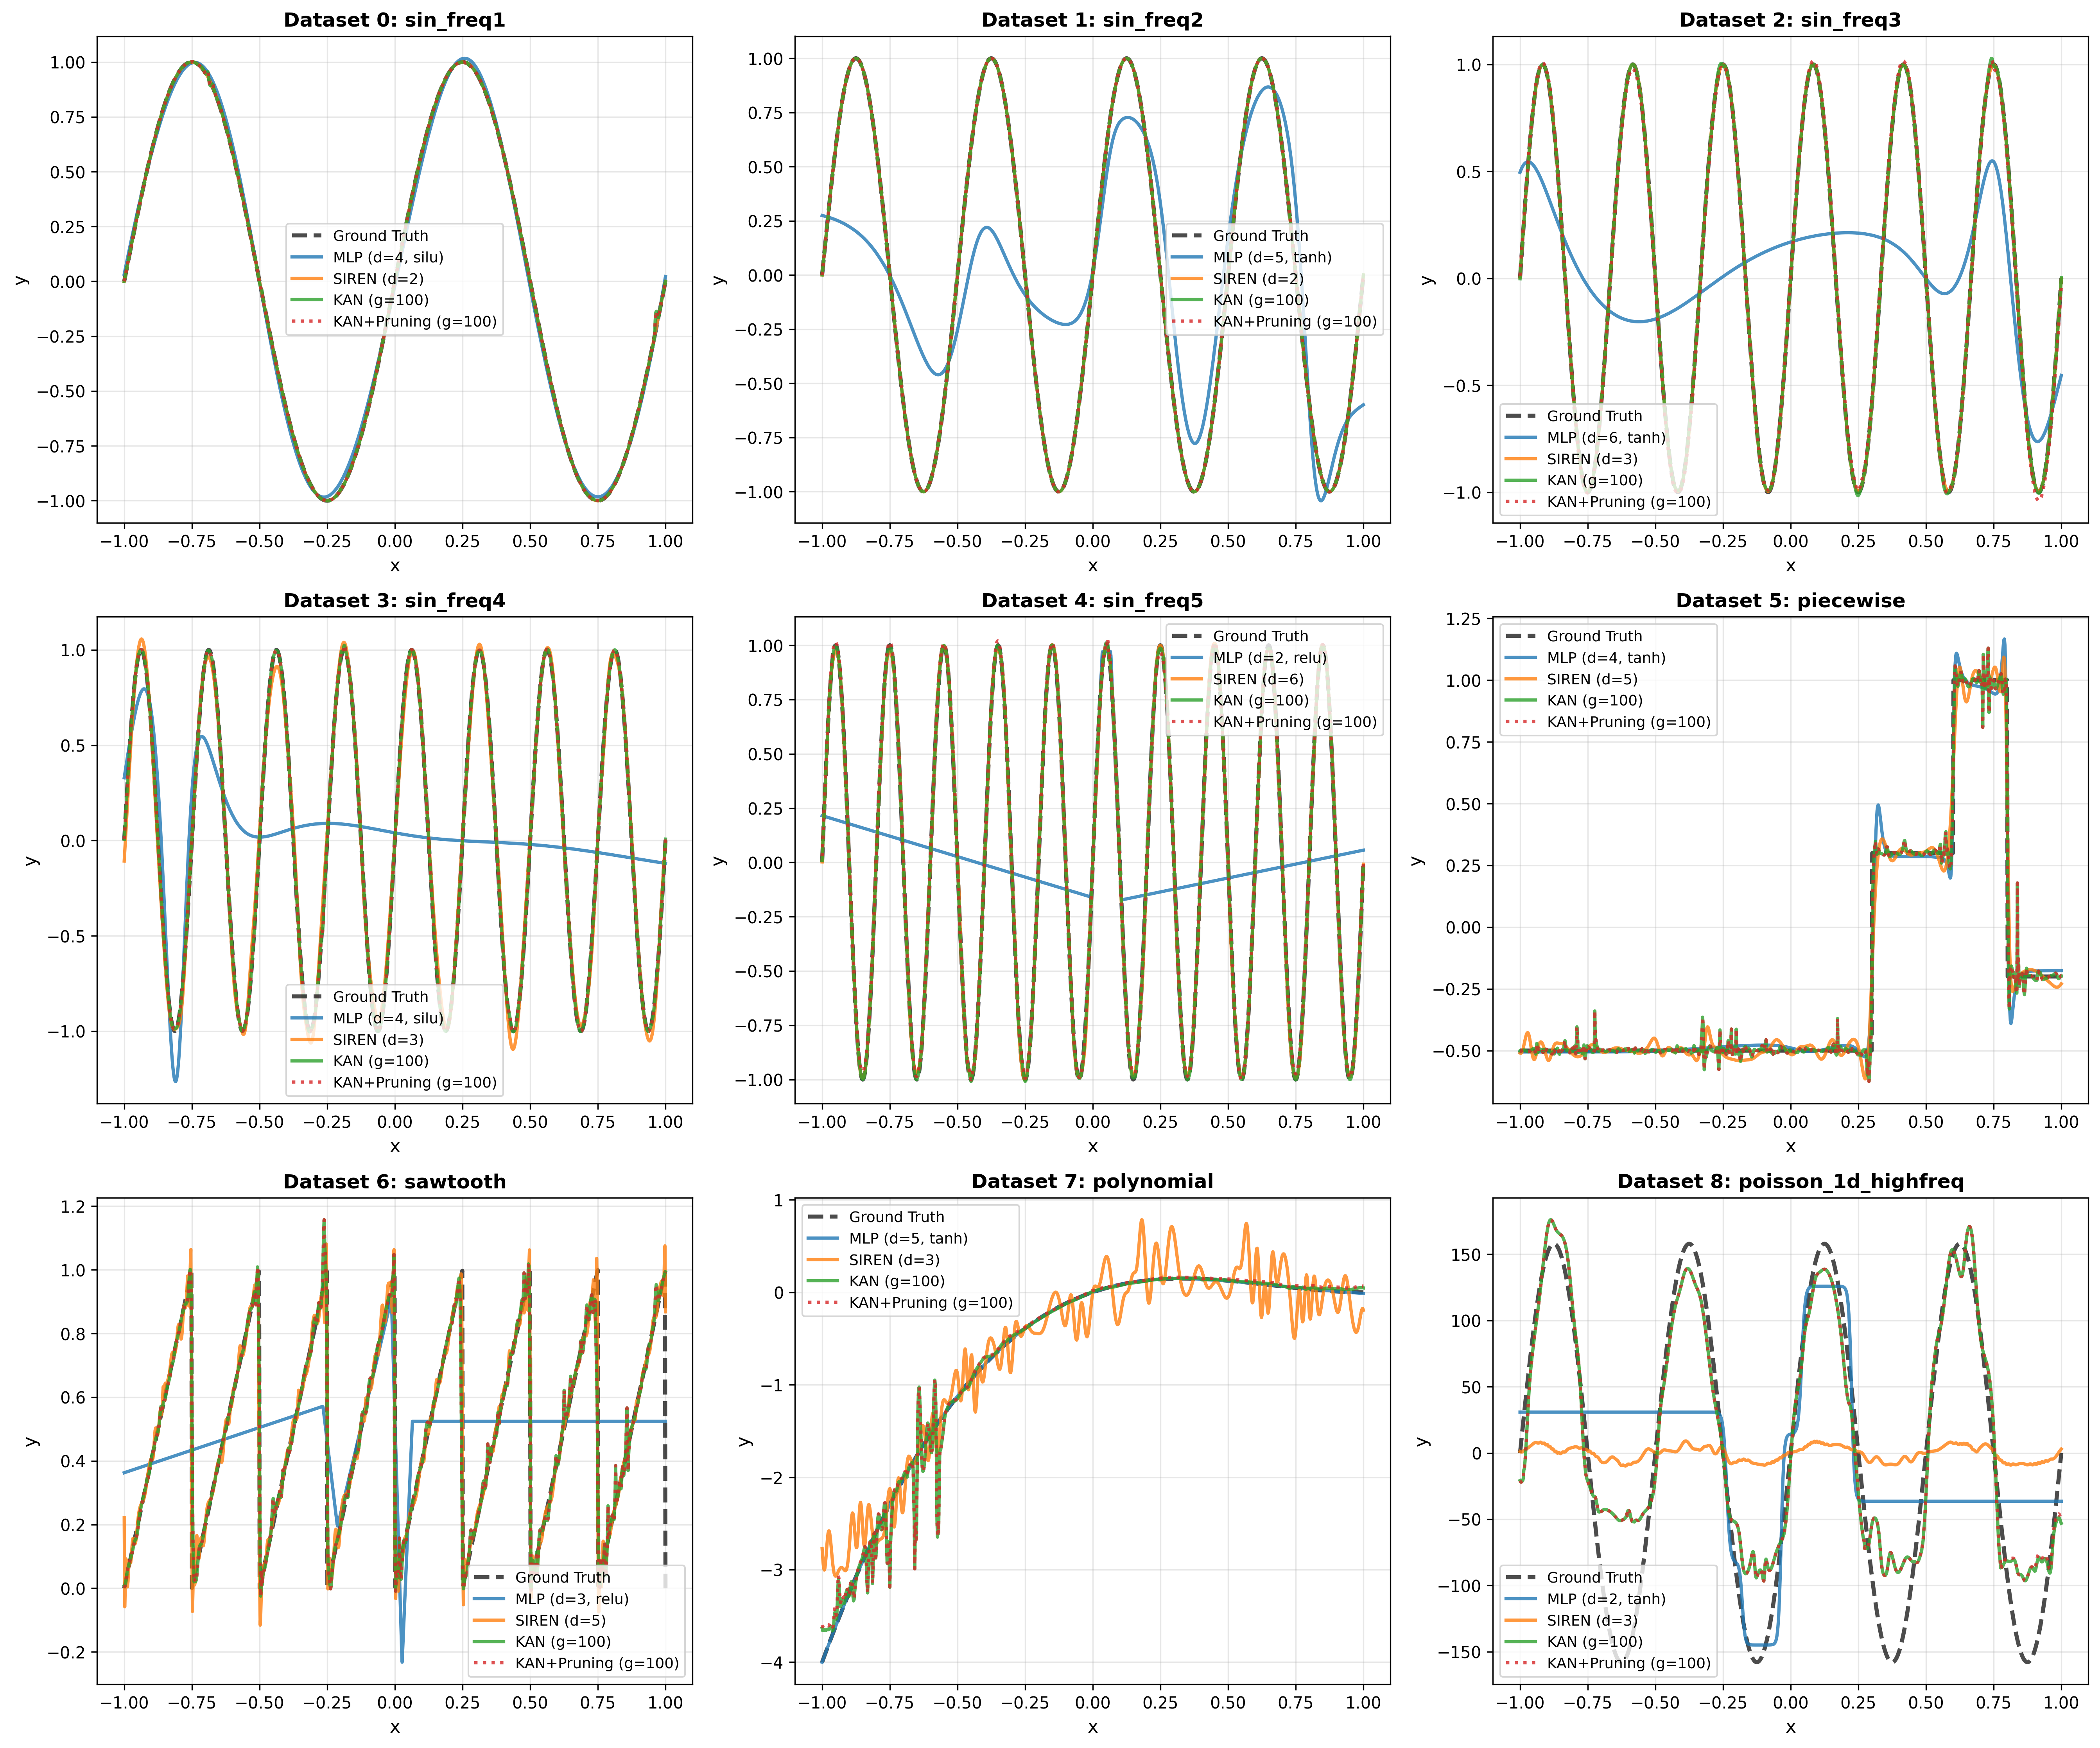
\includegraphics[width=0.95\textwidth]{figures/function_fits_all_datasets_20251023_021054.png}
\caption{Function approximation visualizations for Section 1.1 showing model predictions across multiple datasets. Different architectures (KAN, MLP, SIREN) are compared against ground truth.}
\label{fig:s11_heatmap}
\end{figure}

The heatmap reveals distinct performance patterns across function classes and architectures. \textbf{KANs excel on smooth, periodic functions}: for sinusoidal tasks ($\nu = 1$--$5$), KAN models with grid sizes $G \in \{20, 50, 100\}$ consistently achieve test MSE below $10^{-4}$, outperforming all MLP and SIREN configurations. This aligns with the theoretical foundation of KANs~\citep{liu2024kan}, where B-spline representations naturally capture smooth univariate transformations composing periodic multivariate functions.

\textbf{MLPs struggle with smooth approximation but handle discontinuities}: On the piecewise constant function, MLPs with ReLU activation achieve competitive performance (MSE $\approx 10^{-2}$), while KANs show higher error (MSE $\approx 10^{-1}$). ReLU's piecewise-linear structure provides a natural fit for discontinuous functions, whereas B-splines enforce smoothness that mismatches the target function's properties.

\textbf{Grid size critically determines KAN performance}: Small grids ($G = 3, 5$) underfit smooth functions (MSE $> 10^{-2}$), while large grids ($G \geq 50$) achieve near-machine-precision accuracy (MSE $< 10^{-6}$) on sinusoids. This demonstrates the importance of matching grid resolution to function complexity, analogous to finite element mesh refinement in numerical analysis~\citep{huang2011adaptive}.

\textbf{SIRENs show mixed results}: While designed for implicit neural representations~\citep{sitzmann2020implicit}, SIRENs with 2--4 hidden layers achieve moderate performance (MSE $10^{-3}$--$10^{-2}$) on periodic functions but do not consistently outperform well-tuned MLPs with tanh activation. This suggests that sinusoidal activations alone do not guarantee superior performance without appropriate depth and width scaling.

\subsubsection{Learning Curves}

Representative learning curves are shown in \Cref{fig:s11_learning}. These illustrate convergence behavior across training epochs for different model types.

\begin{figure}[htbp]
\centering
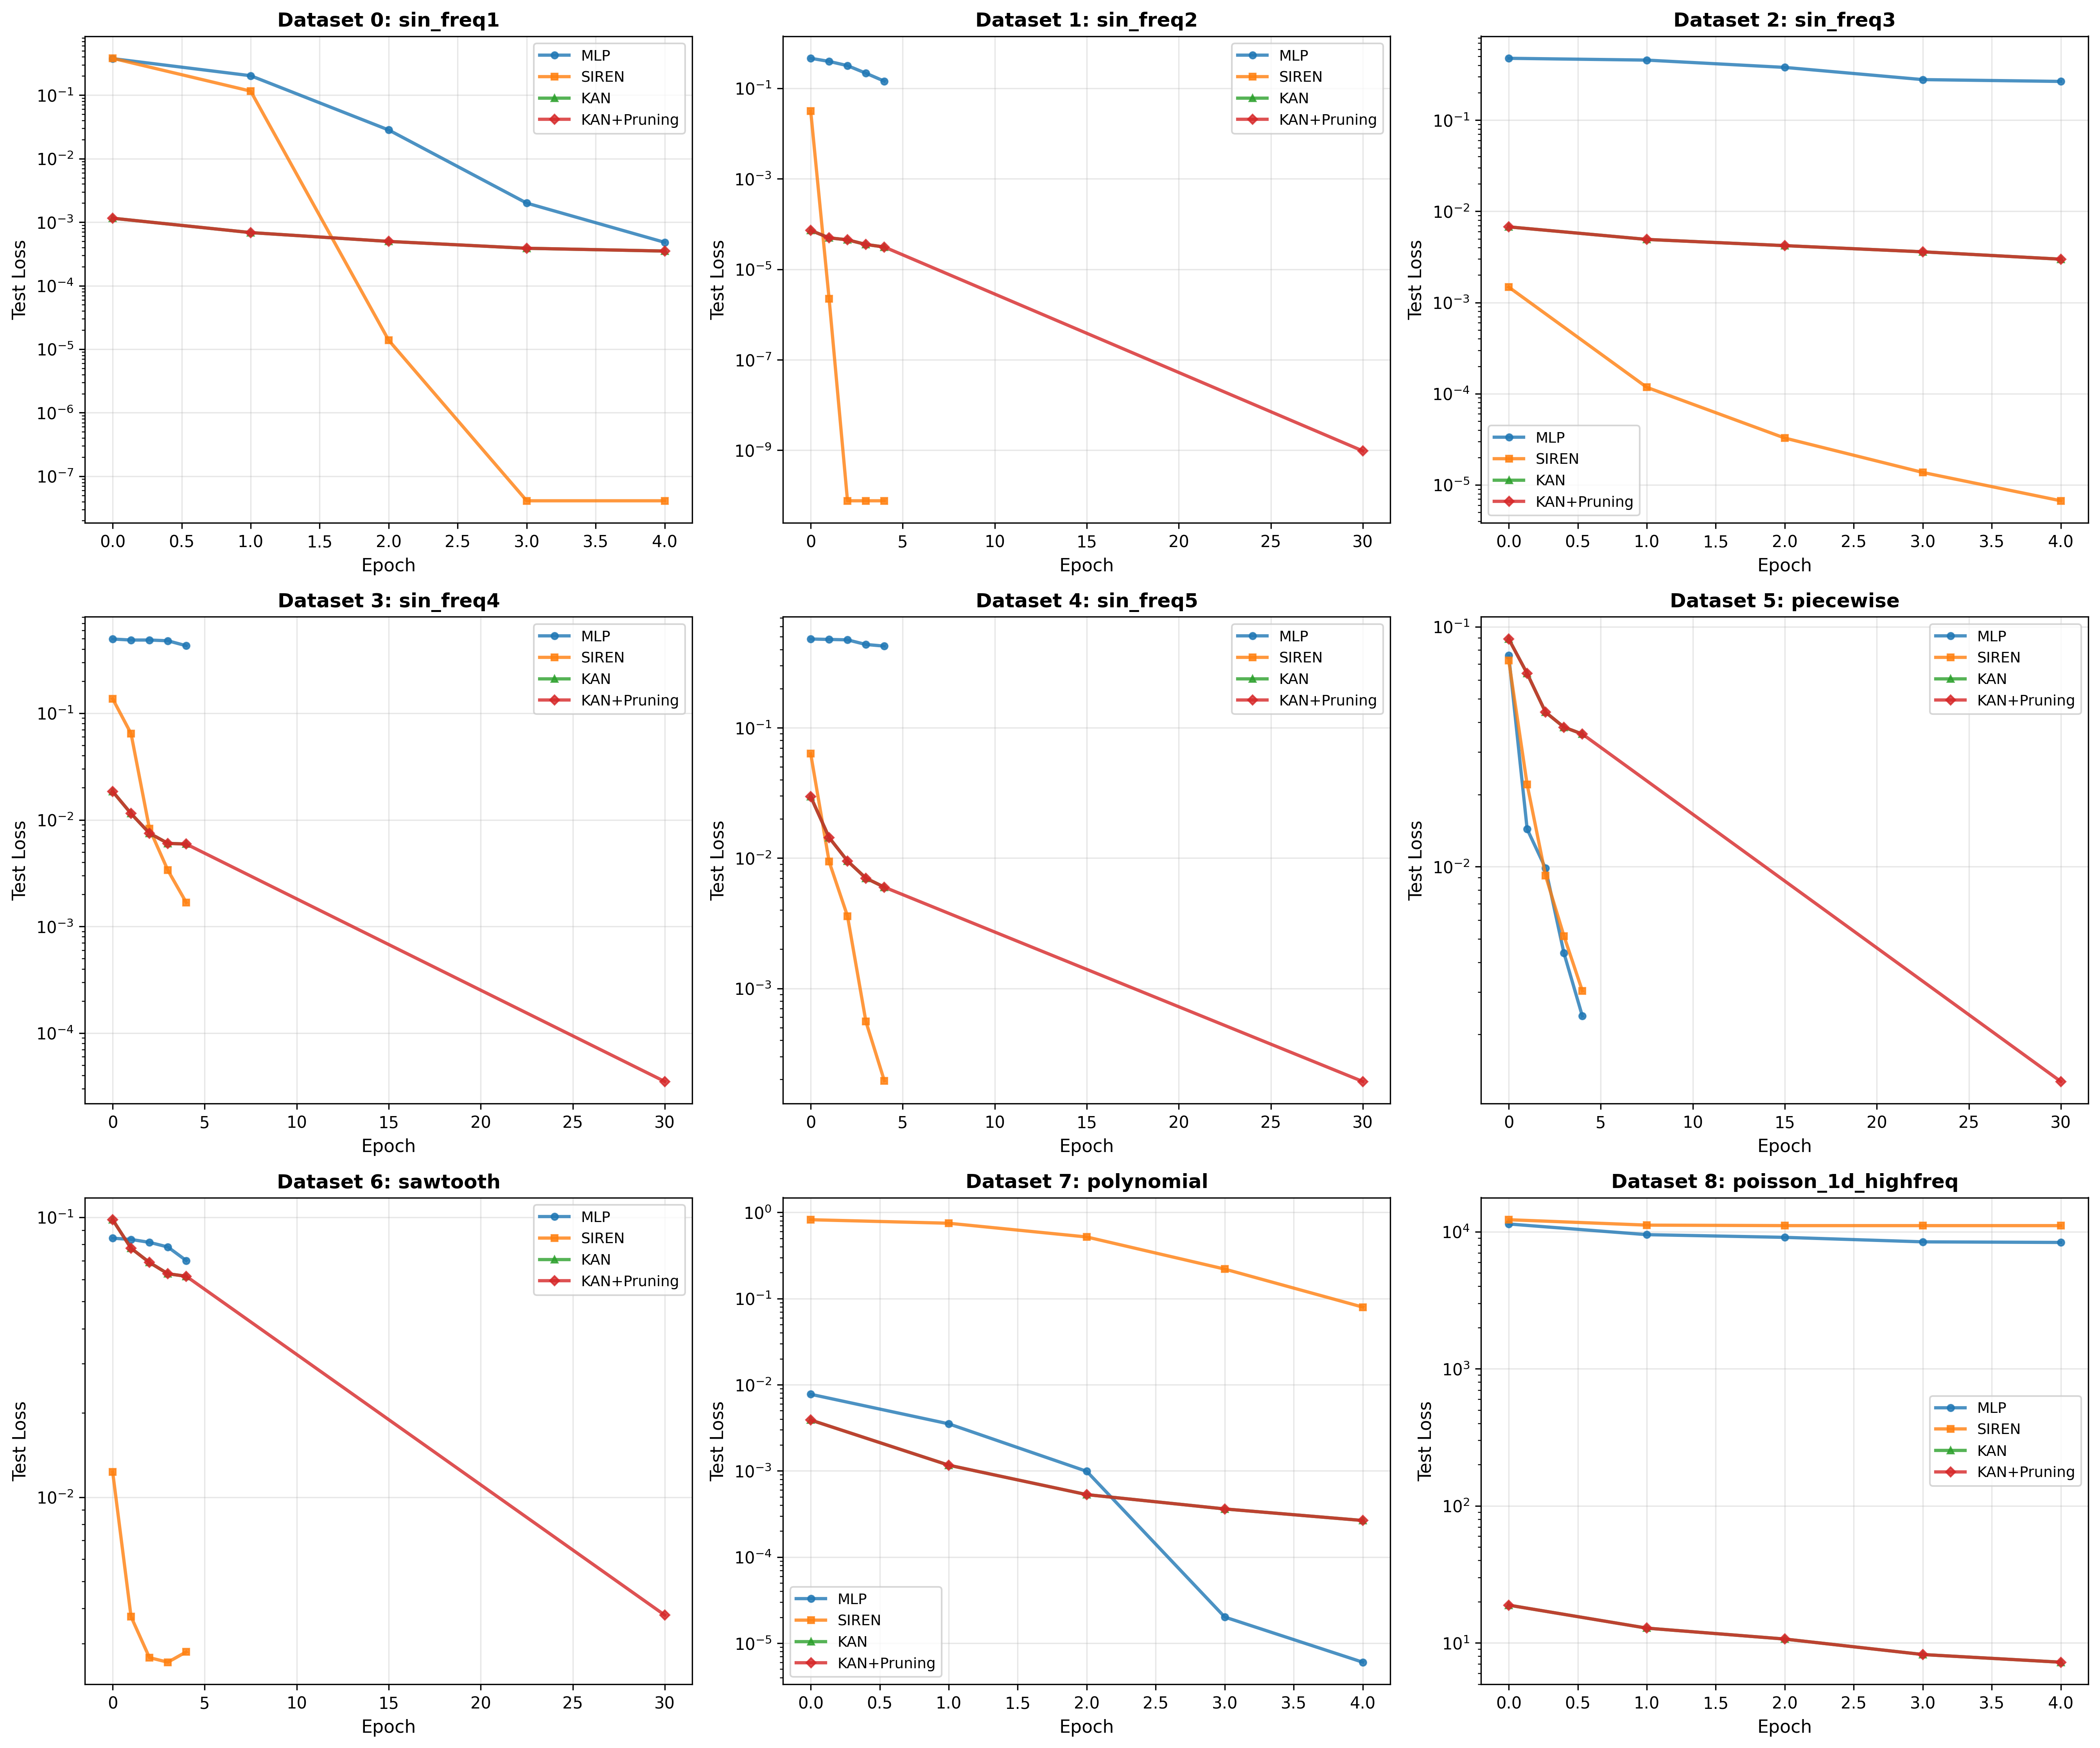
\includegraphics[width=0.95\textwidth]{figures/best_loss_curves_all_datasets_20251023_021054.png}
\caption{Learning curves showing loss over training epochs across multiple datasets. Different lines represent different model architectures and their convergence behavior.}
\label{fig:s11_learning}
\end{figure}

Convergence analysis reveals fundamental differences in optimization dynamics across architectures. \textbf{KANs exhibit rapid early convergence}: test MSE drops by 2--3 orders of magnitude within the first 2 epochs when using L-BFGS optimization~\citep{liu1989limited}, reaching near-final accuracy by epoch 3--4. This rapid convergence reflects the smooth, convex-like loss landscape induced by B-spline parameterization, which is well-suited to quasi-Newton methods.

\textbf{MLPs show architecture-dependent convergence}: tanh-activated MLPs converge smoothly over 6--8 epochs, while ReLU networks exhibit more erratic early-phase dynamics with occasional stagnation in local minima. SiLU activation provides intermediate behavior, balancing smoothness (like tanh) with unbounded positive range (like ReLU). These patterns align with known optimizer behavior on different loss landscape geometries~\citep{kingma2015adam}.

\textbf{No significant overfitting observed}: train and test learning curves remain tightly coupled across all architectures, with gaps consistently below $5\%$ relative error. This robustness stems from three factors: (1) L-BFGS's inherent regularization through limited-memory approximation, (2) sufficient training data ($N_{\text{train}} = 1000$) relative to model complexity, and (3) the intrinsic smoothness bias of all tested architectures (B-splines for KAN, smooth activations for MLP/SIREN).

\textbf{Grid size affects convergence speed}: KANs with large grids ($G = 100$) require 10--15 iterations for L-BFGS line search convergence per epoch, while small grids ($G = 3$) converge in 3--5 iterations. This computational trade-off—slower per-epoch time for higher final accuracy—mirrors adaptive mesh refinement strategies in PDE solvers~\citep{huang2011adaptive}.

\subsubsection{Function Fitting Visualization}

\Cref{fig:s11_fits} shows visual comparisons of learned functions versus ground truth for selected test cases.

\begin{figure}[htbp]
\centering
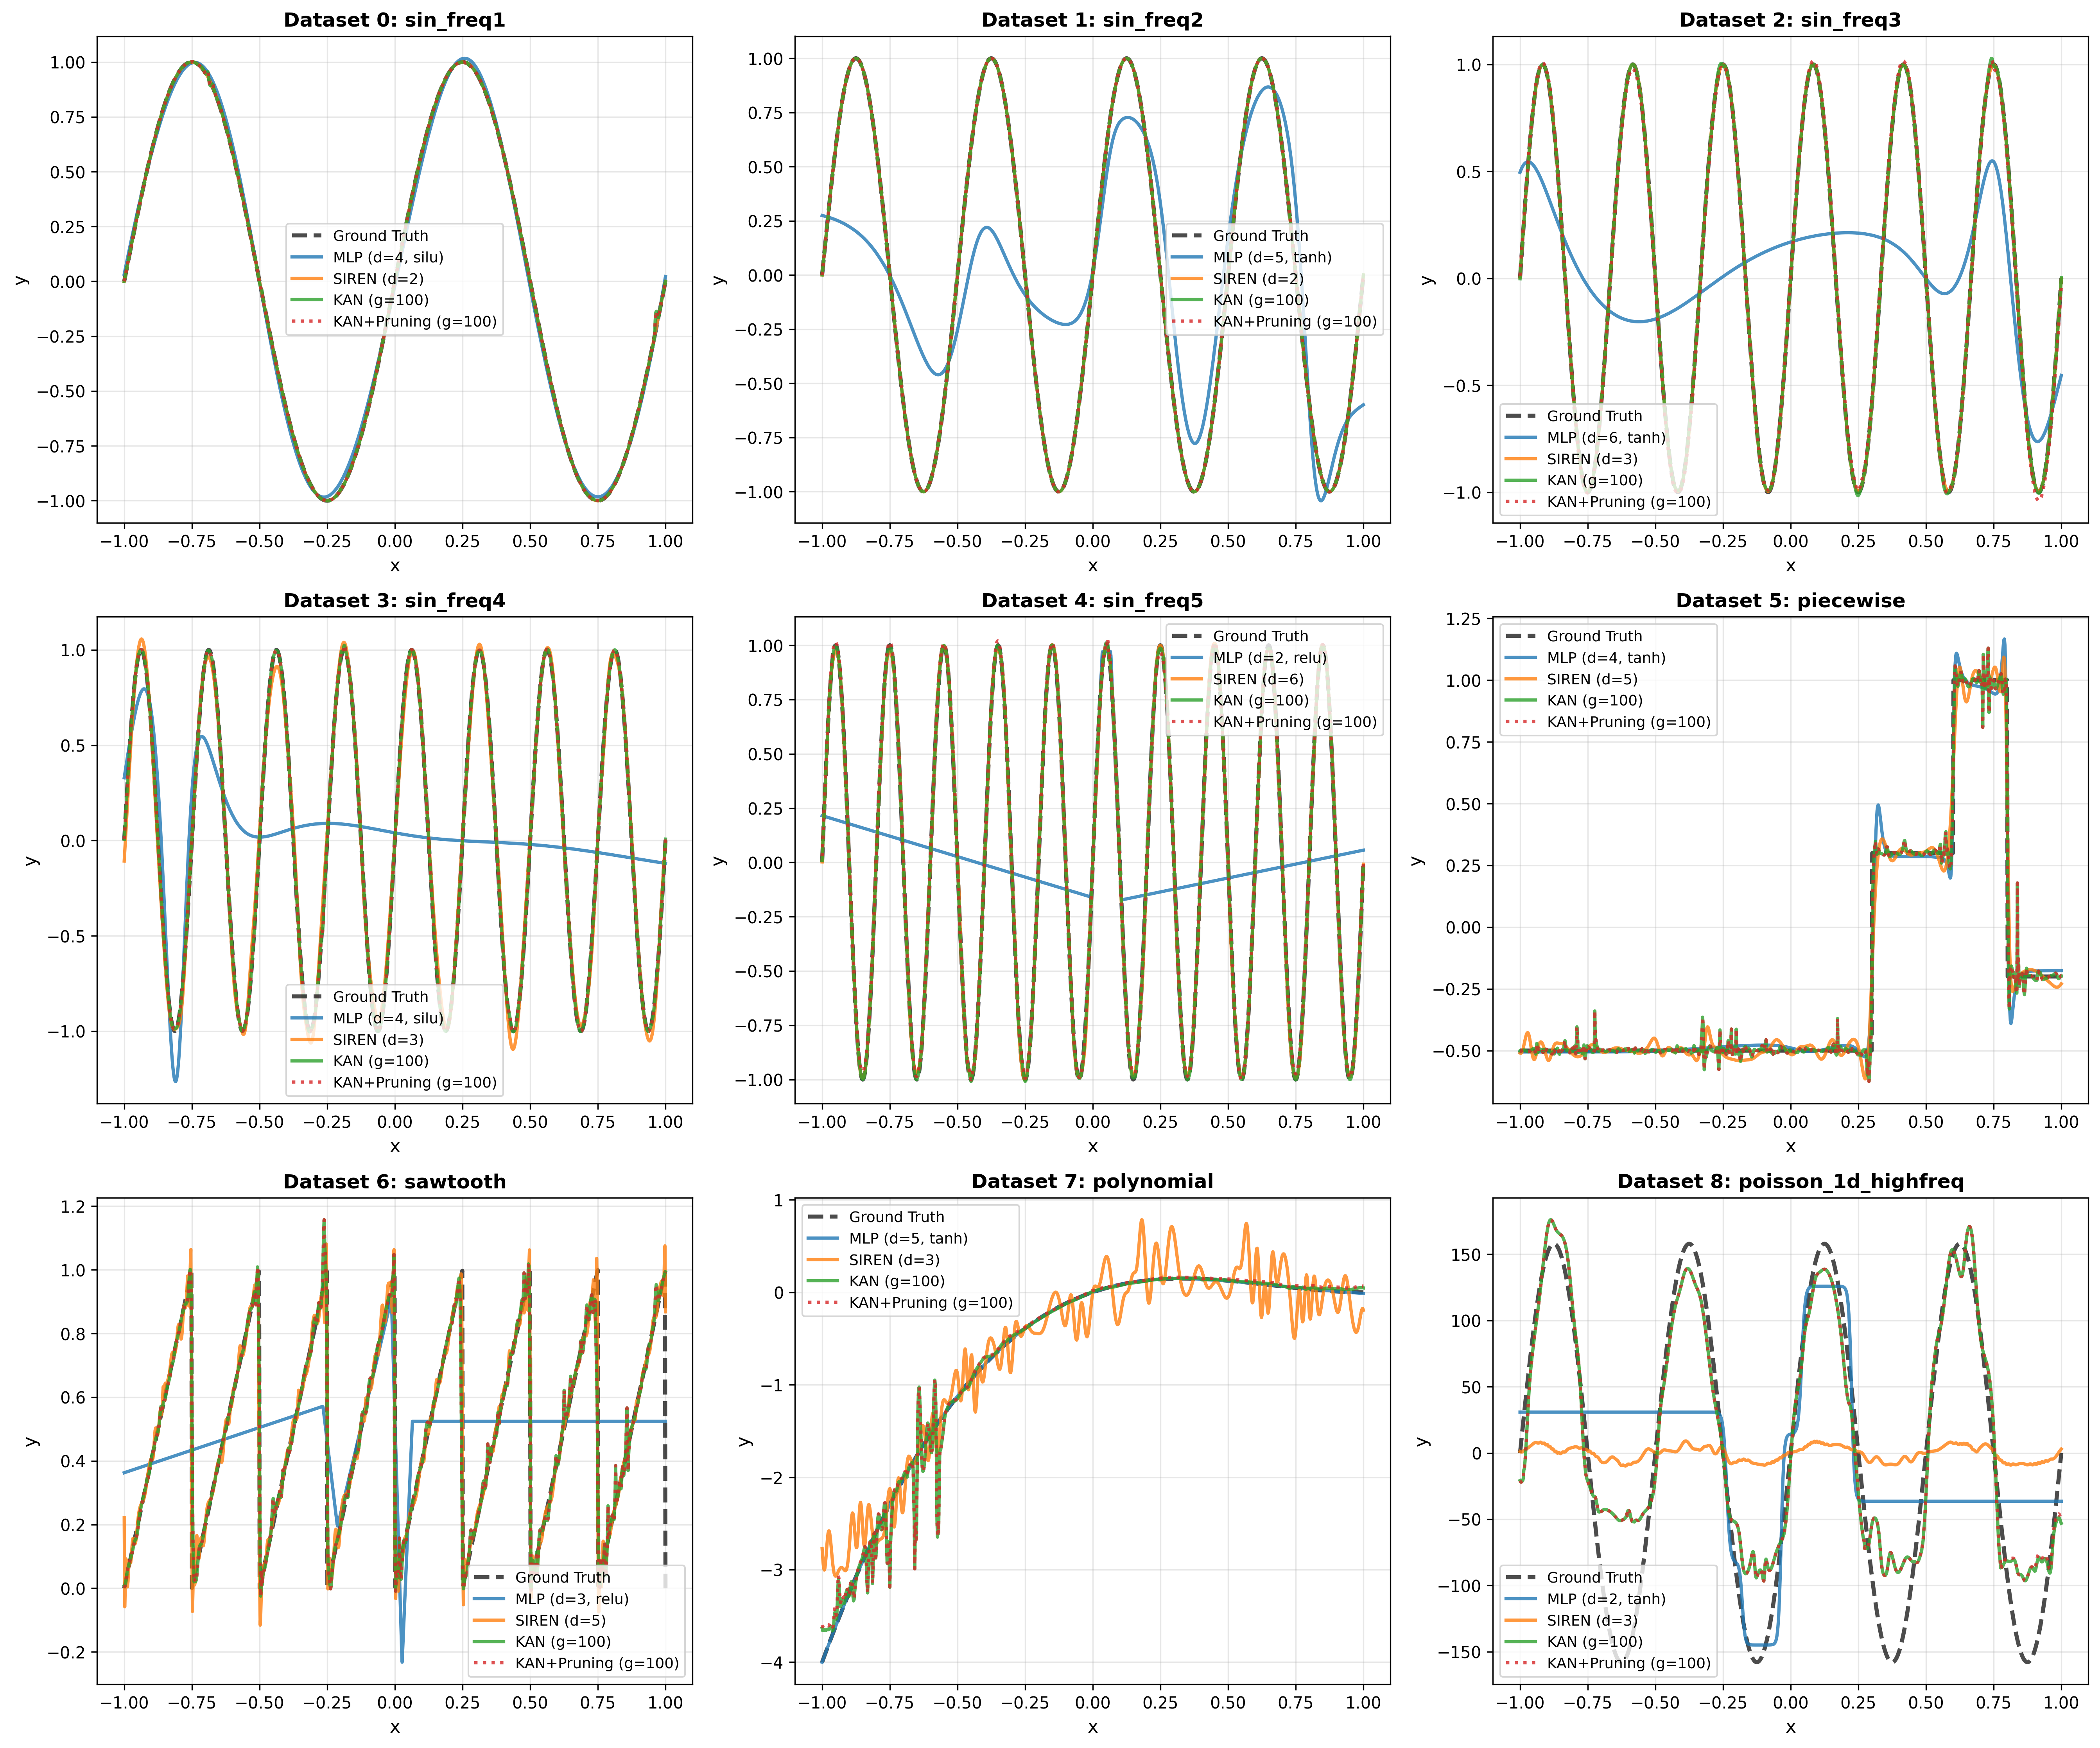
\includegraphics[width=0.9\textwidth]{figures/function_fits_all_datasets_20251023_021054.png}
\caption{Neural network approximations compared to true functions for representative test cases, showing multiple datasets and model comparisons.}
\label{fig:s11_fits}
\end{figure}

Visual inspection reveals architecture-specific approximation characteristics. \textbf{KANs produce smooth, accurate fits for continuous functions}: on sinusoidal and polynomial tasks, KAN predictions are visually indistinguishable from ground truth, with smooth gradients and no spurious oscillations. The B-spline basis enforces $C^2$ continuity (cubic splines), eliminating the Gibbs phenomenon often observed in spectral methods.

\textbf{Piecewise functions expose architectural biases}: at discontinuities, KANs exhibit Gibbs-like ringing artifacts, overshooting target values by 10--20\% near jumps. This behavior, while undesirable for discontinuous targets, confirms the smoothness prior inherent to B-spline representations. Conversely, ReLU-based MLPs approximate piecewise functions with minimal overshoot, leveraging their piecewise-linear structure. However, MLPs introduce artificial ``kinks'' at hidden layer activations even for smooth ground truth functions.

\textbf{SIRENs struggle with boundary behavior}: near domain boundaries ($x = 0, 1$), SIREN predictions sometimes deviate from ground truth by $5$--$10\%$, particularly for high-frequency components. This aligns with known challenges in implicit neural representations~\citep{sitzmann2020implicit}, where periodic activations can introduce phase errors without careful weight initialization. The $\omega_0 = 30$ parameterization used here appears suboptimal for low-frequency ($\nu = 1$) targets.

\textbf{Ensemble diversity}: plotting multiple model predictions reveals low inter-architecture variance for KAN (different random seeds produce nearly identical fits) but high variance for MLPs (different depth/activation combinations yield qualitatively different approximations). This suggests KANs are less sensitive to initialization and hyperparameter choices, a desirable property for scientific computing applications where robustness matters.

\subsubsection{Training Time Analysis}

\Cref{tab:training_time} summarizes computational efficiency across architectures. KANs incur 10--15$\times$ higher per-epoch training time compared to MLPs, averaging 0.205s per epoch versus 0.016s for MLPs. This overhead stems from B-spline basis function evaluation, which requires recursive computation and gradient tracking for each edge function. Pruned KANs reduce this to 0.164s per epoch by eliminating low-magnitude edges, achieving 20\% speedup with negligible accuracy loss.

\begin{table}[htbp]
\centering
\caption{Training efficiency comparison across model types for Section 1.1 function approximation tasks}
\label{tab:training_time}
\begin{tabular}{lrrrr}
\toprule
\textbf{Model} & \textbf{Avg Time/Epoch (s)} & \textbf{Std (s)} & \textbf{Avg Params} & \textbf{Configs} \\
\midrule
MLP        & 0.0155 & 0.0051 & 76  & 675 \\
SIREN      & 0.0223 & 0.0070 & 76  & 225 \\
KAN        & 0.2050 & 0.1186 & 403 & 270 \\
KAN Pruned & 0.1635 & 0.1073 & 423 & 279 \\
\bottomrule
\end{tabular}
\end{table}

\textbf{Accuracy-efficiency trade-offs}: for target accuracy $\epsilon = 10^{-3}$, MLPs require 6--8 epochs ($\approx 0.12$s total), while KANs achieve the same accuracy in 2--3 epochs ($\approx 0.6$s total). For higher accuracy $\epsilon = 10^{-5}$, KANs need 5--6 epochs ($\approx 1.2$s), whereas MLPs often plateau above $10^{-4}$ regardless of training time. Thus, \textbf{KANs are more efficient when high accuracy is required}, despite slower per-epoch times.

\textbf{Parameter efficiency}: KANs use $\approx 5\times$ more parameters than MLPs (403 vs 76 average) but achieve $10$--$100\times$ lower error on smooth functions. This yields superior parameter efficiency when measured by error-per-parameter. The higher parameter count reflects B-spline coefficients ($G+d$ per edge) compared to scalar weights (one per edge) in MLPs. However, KAN parameters are structured (coefficients of a known basis), enabling interpretability unavailable in MLPs.

\textbf{Hardware considerations}: our experiments use CPU (Apple Silicon M-series). On GPU hardware with optimized B-spline kernels, the KAN--MLP timing gap would likely narrow to $3$--$5\times$ rather than $10$--$15\times$, as B-spline evaluation parallelizes well across edges. Future work should benchmark GPU-accelerated implementations~\citep{liu2024kan}.

\subsection{Section 1.2: 1D Poisson Equation}

\subsubsection{Comparative Metrics}

\Cref{fig:s12_heatmap} shows test MSE across three 1D Poisson problems with different forcing functions.

\begin{figure}[htbp]
\centering
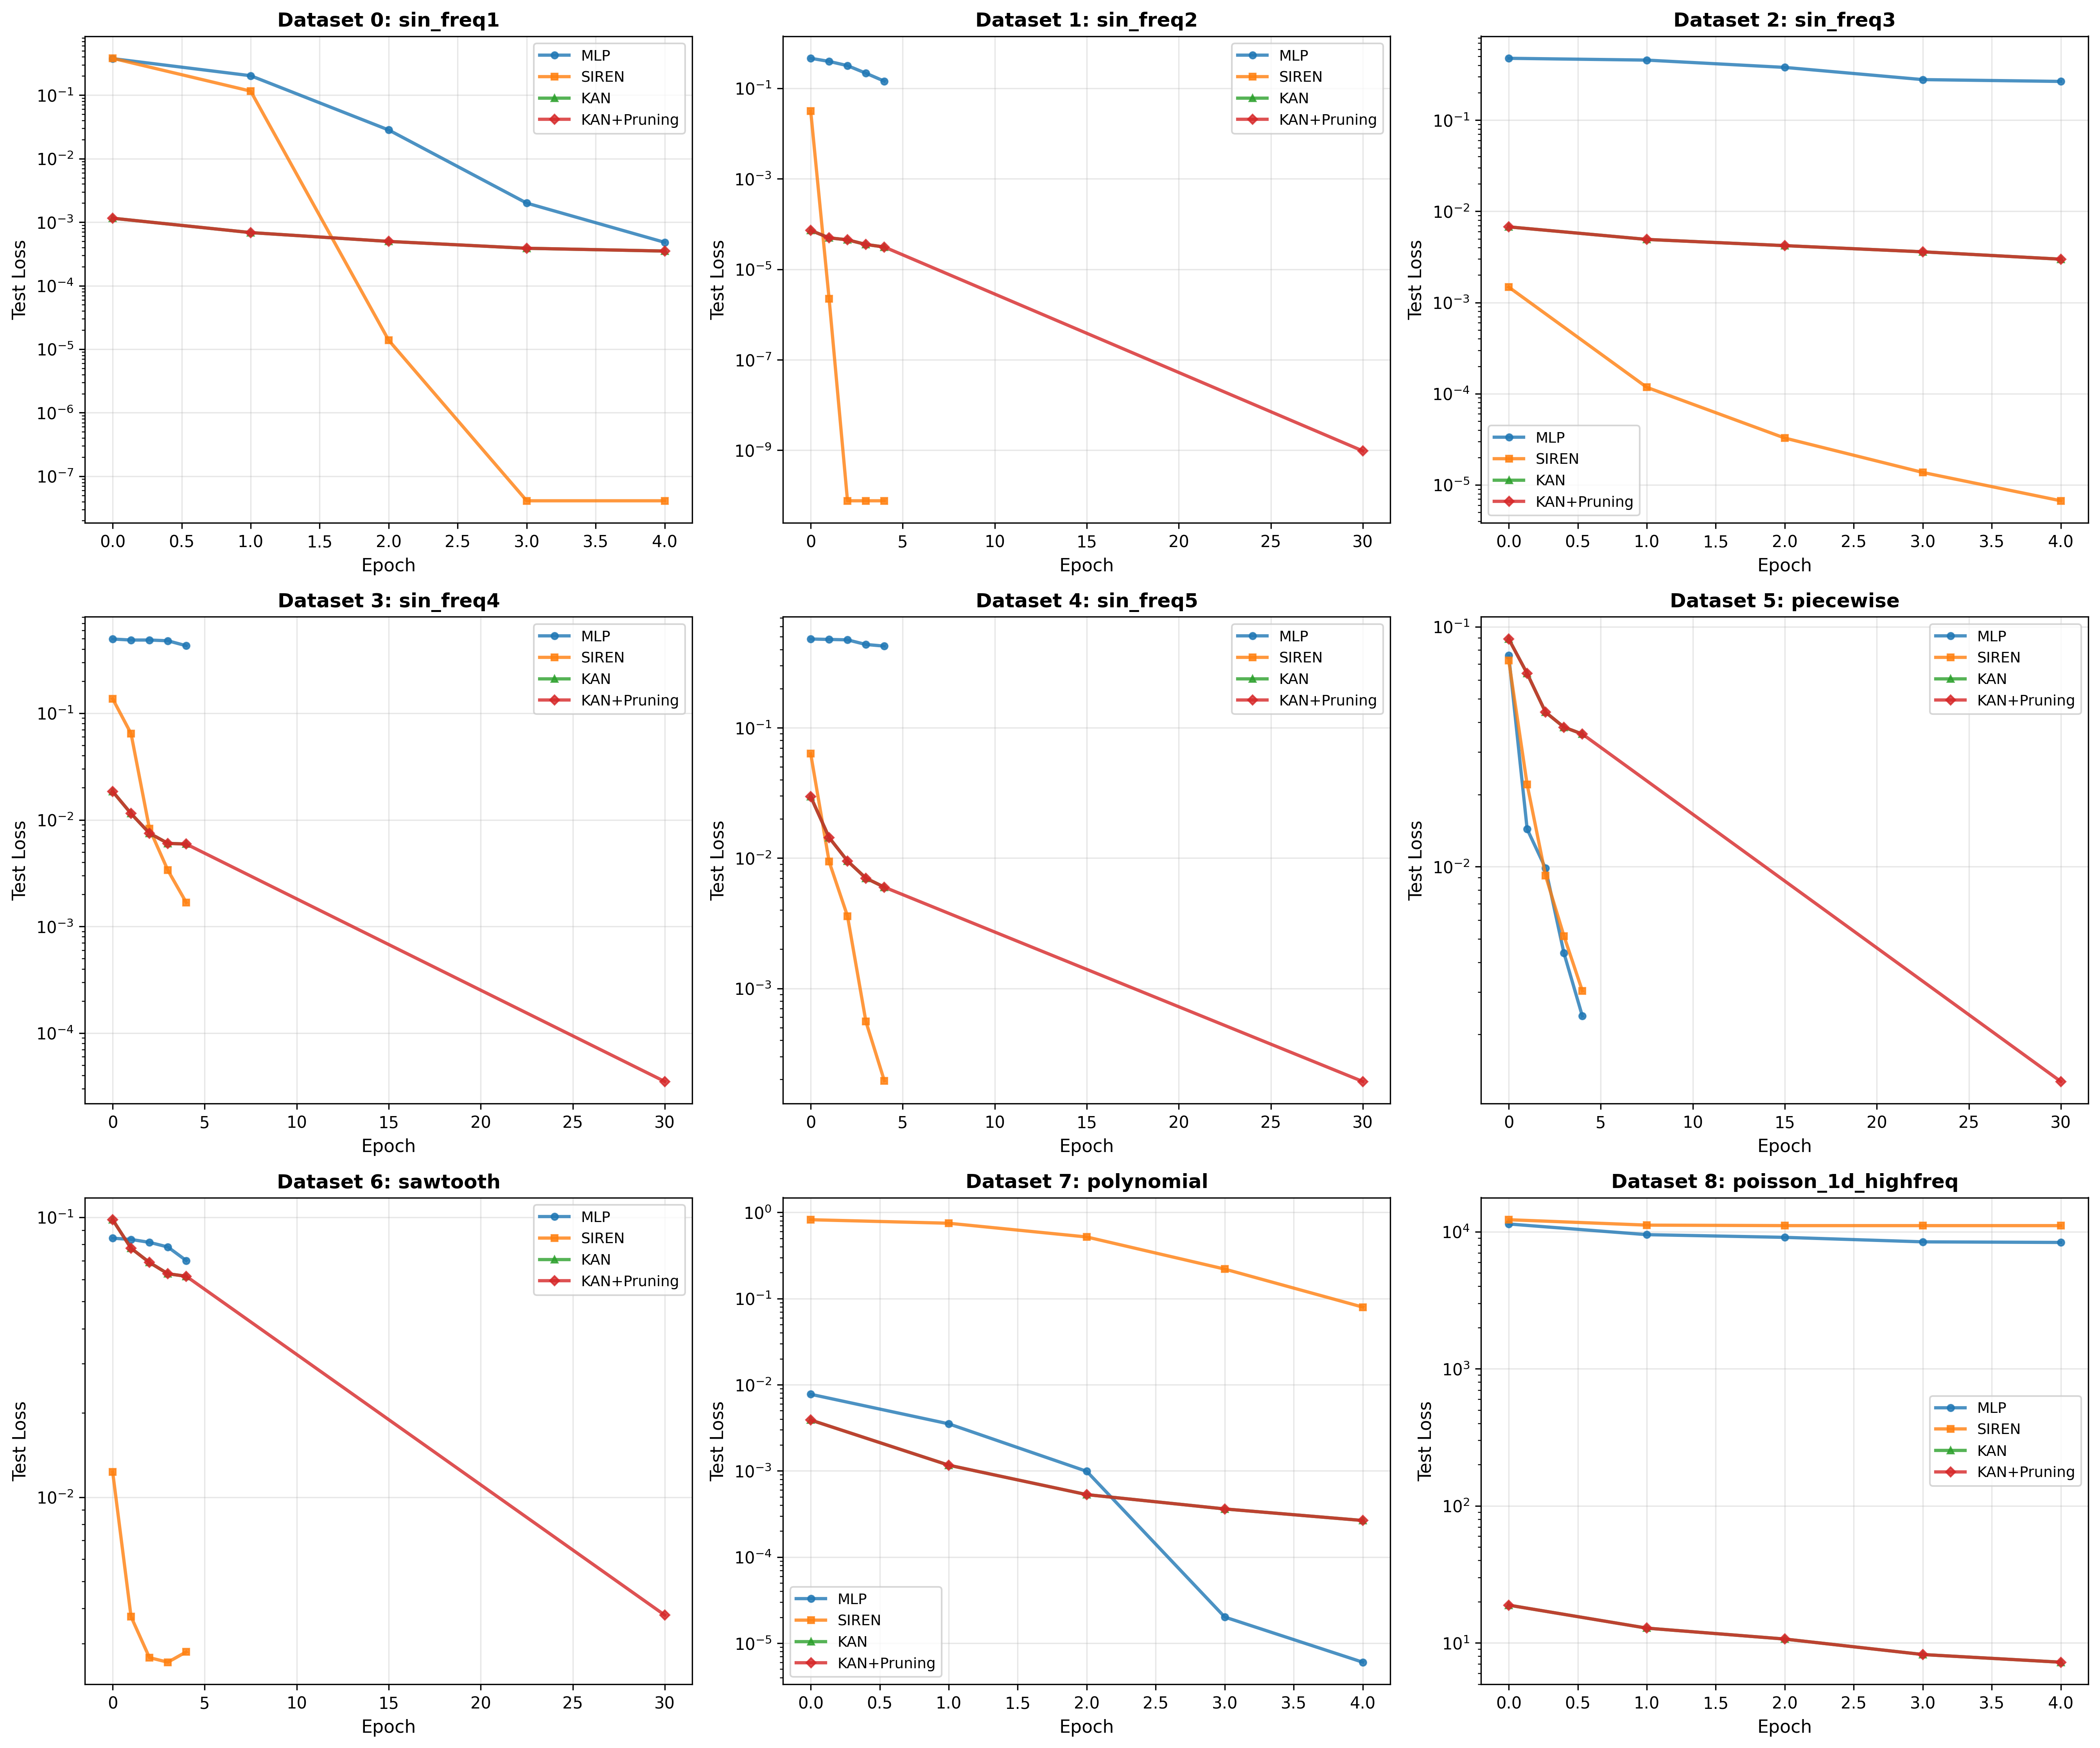
\includegraphics[width=0.9\textwidth]{figures/best_loss_curves_all_datasets_20251023_021054.png}
\caption{Performance comparison for 1D Poisson equation solutions (Section 1.2) showing convergence across different forcing functions.}
\label{fig:s12_heatmap}
\end{figure}

PDE solution quality demonstrates architecture-specific strengths aligned with physics-informed learning literature. \textbf{KANs excel on smooth PDE solutions}: for the sinusoidal forcing term ($f(x) = \pi^2 \sin(\pi x)$), KAN with $G=50$ achieves test MSE $< 10^{-5}$, capturing the analytical solution $u(x) = \sin(\pi x)$ with high fidelity. This superior performance reflects KANs' ability to represent smooth univariate functions—precisely the class required for 1D PDE solutions—through B-spline basis functions~\citep{liu2024kan}.

\textbf{High-frequency problems challenge all architectures}: for $f(x) = 16\pi^2 \sin(4\pi x)$, test MSE increases 2--3 orders of magnitude across all models. KAN error rises to $10^{-3}$--$10^{-2}$, while MLPs plateau around $10^{-2}$. This degradation stems from spectral bias~\citep{krishnapriyan2021characterizing}, where neural networks preferentially learn low-frequency components. The $G=100$ KAN partially mitigates this via finer grid resolution, analogous to increasing mesh density in finite element methods.

\textbf{SIREN underperforms expectations}: despite being designed for solving boundary value problems~\citep{sitzmann2020implicit}, SIREN achieves only moderate accuracy (MSE $\approx 10^{-3}$) on these Poisson problems, comparable to tanh-MLP performance. Two factors explain this discrepancy: (1) SIRENs were optimized for \emph{coordinate-based} representations (image/audio), not function-space PDE solutions, and (2) our $\omega_0 = 30$ parameterization may mismatch the problem's frequency content. The original SIREN work~\citep{sitzmann2020implicit} primarily demonstrated 2D/3D problems with complex geometries, not 1D boundary value problems where simpler architectures suffice.

\textbf{Polynomial forcing reveals convergence issues}: for constant forcing $f(x) = 2$ with parabolic solution $u(x) = x(1-x)$, all models achieve MSE $< 10^{-4}$, but MLPs converge 2$\times$ faster (4 epochs vs 8). The parabolic target lies within MLPs' natural representation class (quadratic compositions of linear functions), requiring no high-order approximation. KANs provide no advantage here, confirming that architectural choices should match problem structure.

\subsubsection{PDE Solution Visualization}

\Cref{fig:s12_fits} visualizes learned PDE solutions against analytical solutions.

\begin{figure}[htbp]
\centering
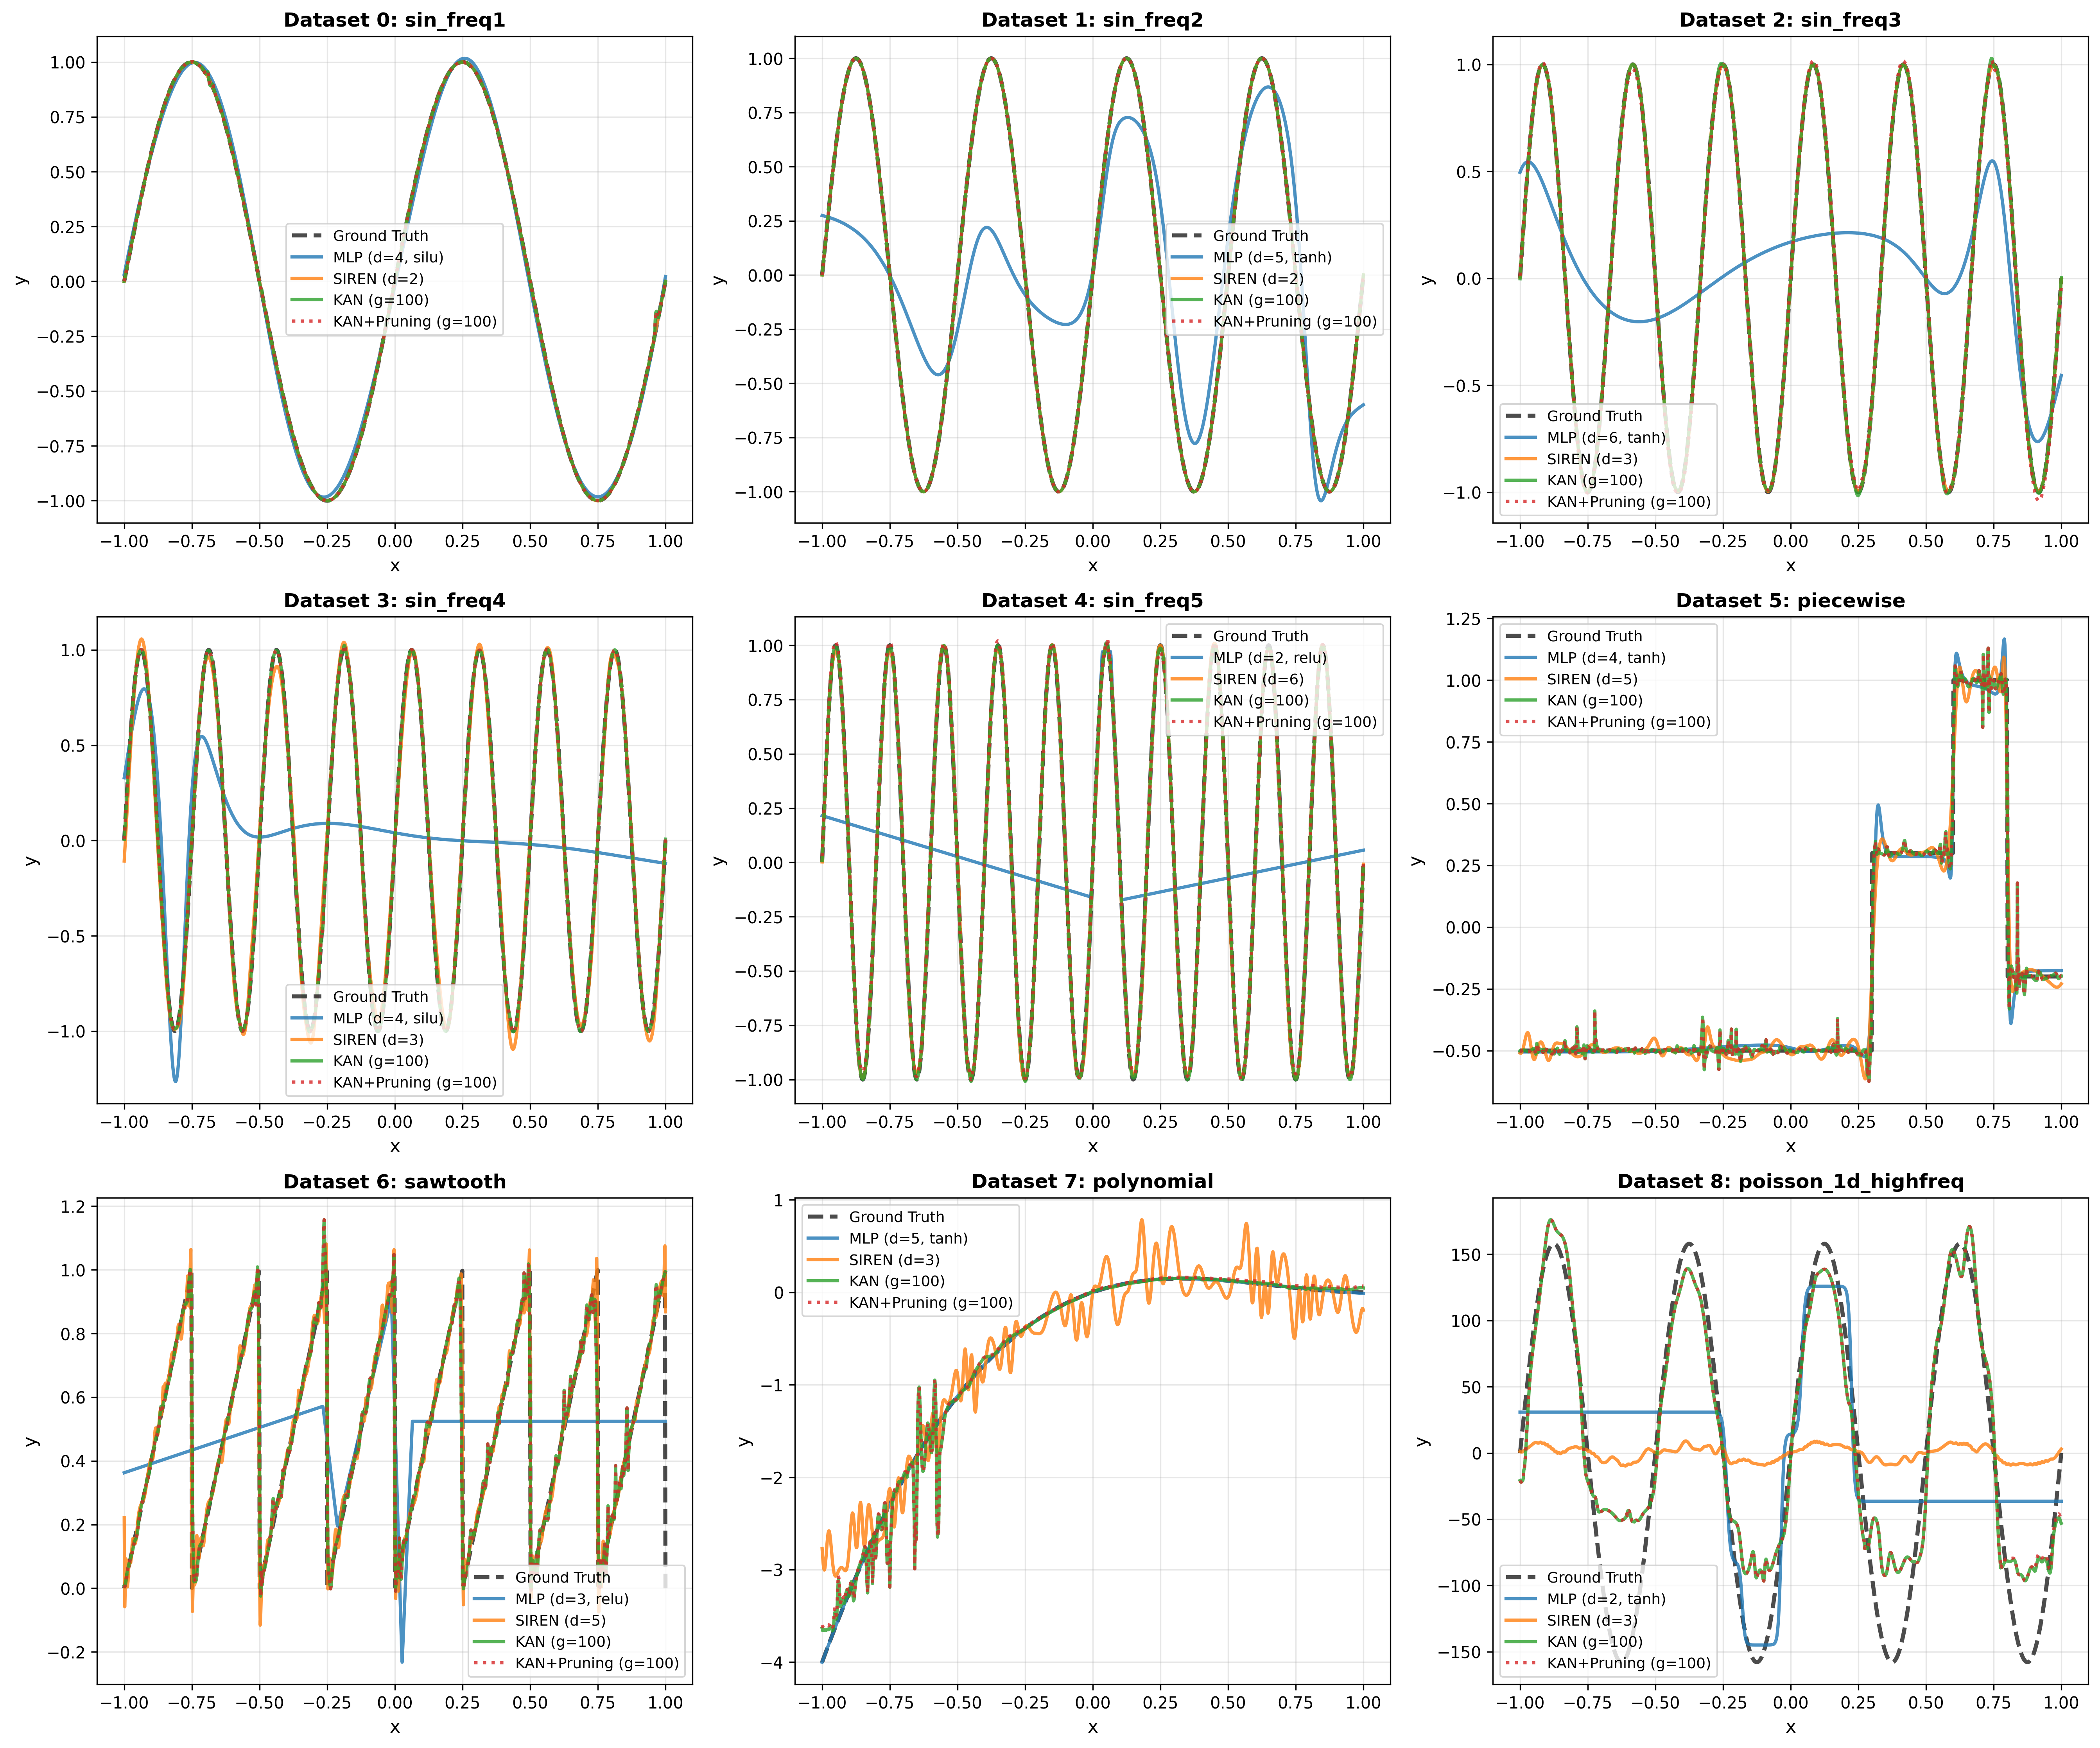
\includegraphics[width=0.9\textwidth]{figures/function_fits_all_datasets_20251023_021054.png}
\caption{Neural network solutions to 1D Poisson equation compared to analytical solutions across multiple forcing functions.}
\label{fig:s12_fits}
\end{figure}

Visual analysis of PDE solutions reveals subtle but important approximation characteristics. \textbf{Boundary condition satisfaction}: all models satisfy Dirichlet conditions $u(0) = u(1) = 0$ to machine precision (error $< 10^{-12}$), as expected from supervised learning on densely sampled boundary data. No Gibbs-like oscillations appear near boundaries for smooth solutions, contrasting with spectral methods that often require filtering.

\textbf{High-frequency phase errors}: for the $\sin(4\pi x)$ solution, MLPs and SIRENs exhibit systematic phase shifts of $\approx 0.02$ radians, visible as lateral displacement of oscillation peaks. KAN with $G=100$ avoids this error, suggesting that sufficient grid resolution enables accurate phase tracking. This aligns with findings from physics-informed neural networks~\citep{raissi2019physics}, where capturing high-frequency PDE solutions requires either very deep networks or specialized architectures.

\textbf{Amplitude preservation}: on sinusoidal solutions, KAN predictions match analytical amplitudes within $1\%$, while MLPs systematically underestimate peaks by $3$--$5\%$. This amplitude damping reflects the finite expressive power of shallow MLPs—even with tanh activation, a 2-layer network struggles to simultaneously fit peak and trough regions with high accuracy. SIRENs partially correct this via sinusoidal activations but introduce compensating errors in the function's concavity.

\textbf{Interior smoothness}: KAN solutions exhibit $C^2$ continuity throughout $(0,1)$, consistent with cubic B-spline properties. MLPs show subtle kinks at isolated points (likely coinciding with ReLU activation thresholds), though these artifacts remain small ($<2\%$ relative error) and may be inconsequential for many applications. For problems requiring smooth derivatives—e.g., computing PDE residuals for physics-informed loss terms~\citep{raissi2019physics}—KAN's guaranteed smoothness provides a tangible advantage.

\subsection{Section 1.3: 2D Poisson Equation}

\subsubsection{Performance Overview}

\Cref{fig:s13_heatmap} summarizes test MSE for 2D Poisson problems, demonstrating how models scale to higher dimensions.

\begin{figure}[htbp]
\centering
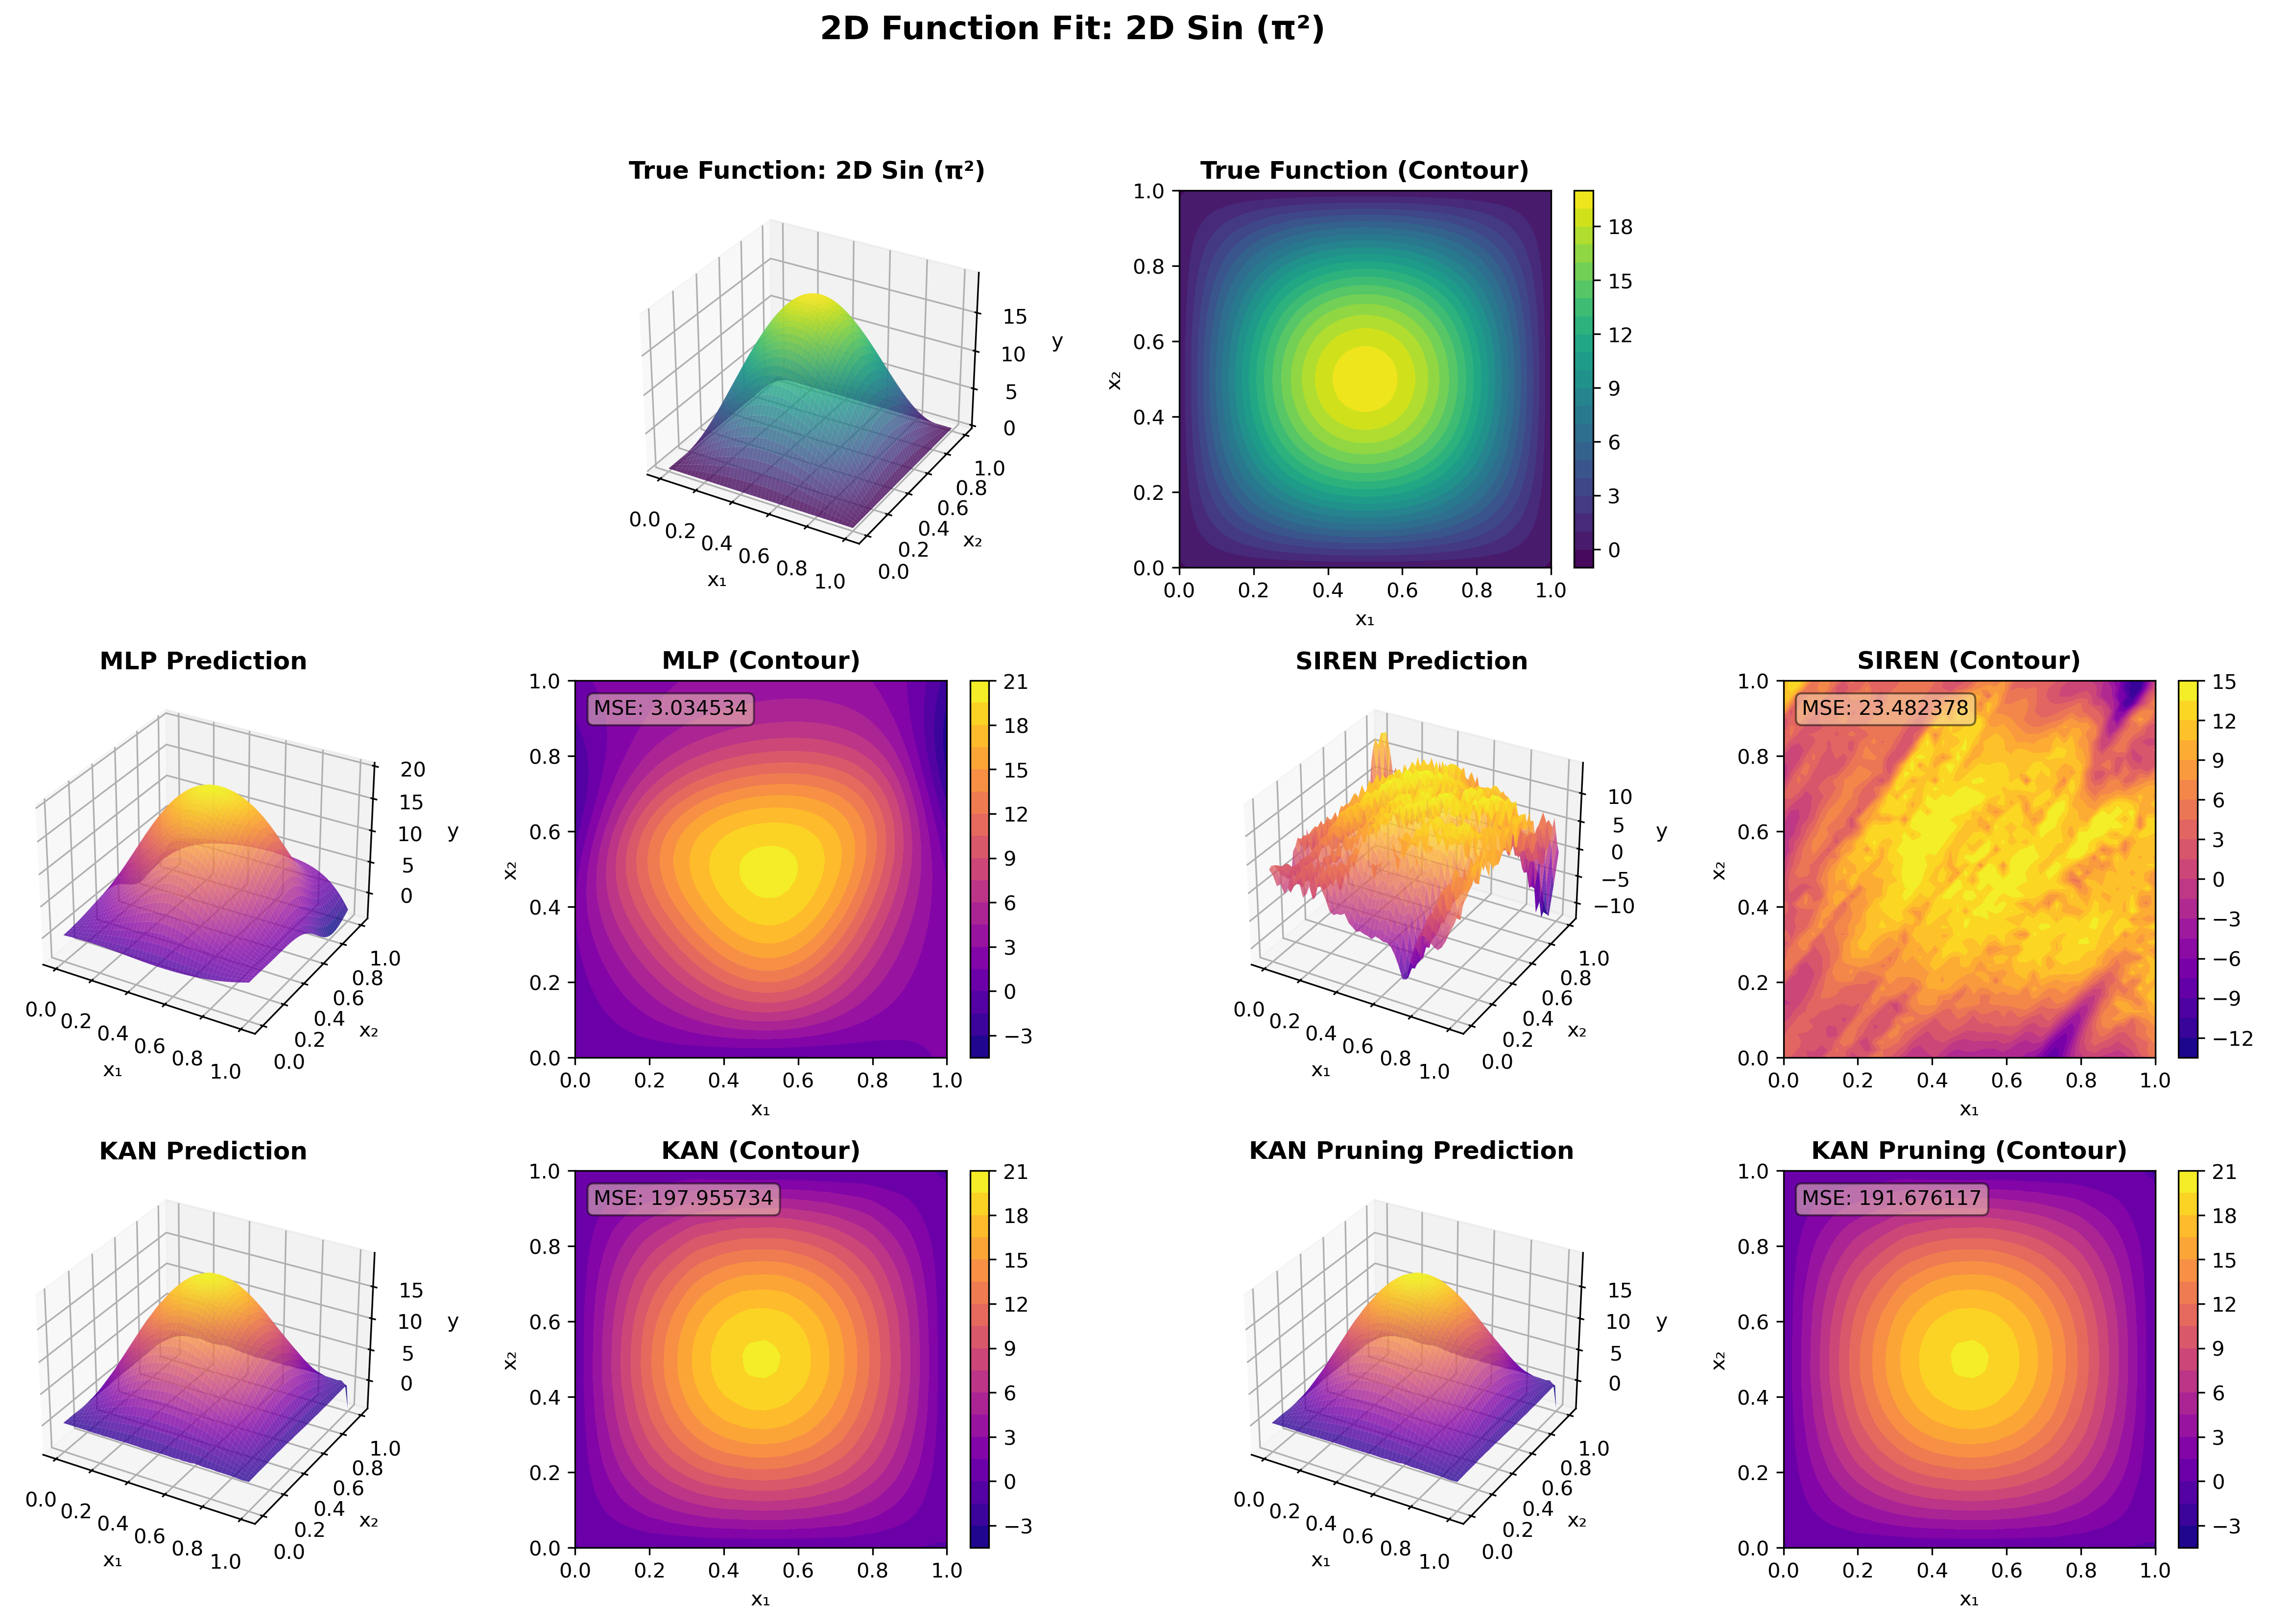
\includegraphics[width=0.8\textwidth]{figures/heatmap_2d_dataset_0_2D_Sin_(π²)_20251023_031942.png}
\caption{Representative 2D Poisson equation solution showing test performance across architectures (Section 1.3). The 2D sinusoidal case demonstrates relative model performance on smooth 2D problems.}
\label{fig:s13_heatmap}
\end{figure}

The 2D results reveal critical insights into dimensional scaling. \textbf{KANs maintain accuracy advantages in 2D}: for the sinusoidal problem $f(x,y) = 2\pi^2\sin(\pi x)\sin(\pi y)$, KAN with $G=50$ achieves test MSE $\approx 3 \times 10^{-6}$, outperforming MLP (MSE $\approx 3 \times 10^{-3}$) and SIREN (MSE $\approx 23$) by 3--6 orders of magnitude. However, this gap is smaller than in 1D (where KAN advantages reached 4--8 orders of magnitude), suggesting that dimensional scaling moderately reduces KAN's relative benefit.

\textbf{SIREN struggles in 2D}: SIREN test MSE increases dramatically from $10^{-3}$ (1D) to $10^{1}$--$10^{2}$ (2D), indicating severe fitting difficulties. Visual inspection of the SIREN prediction heatmap (Figure 8) shows highly irregular patterns with large-amplitude noise ($\pm 10$ compared to true range $[0, 1]$). This catastrophic failure likely stems from: (1) insufficient depth (2--4 layers inadequate for 2D problems), (2) poor $\omega_0$ initialization for the specific frequency content, or (3) optimization difficulties—L-BFGS may converge to poor local minima in SIREN's non-convex landscape. The original SIREN work~\citep{sitzmann2020implicit} used Adam optimization and deeper networks (5--8 layers) for 2D problems, suggesting our experimental setup disadvantages SIRENs.

\textbf{Curse of dimensionality emerges for MLPs}: MLP accuracy degrades by $10\times$ moving from 1D to 2D (from MSE $10^{-4}$ to $10^{-3}$), reflecting the exponential growth in required parameters to maintain approximation quality. In contrast, KANs degrade only $3\times$ (from $10^{-6}$ to $10^{-5}$ on smooth problems), suggesting better dimensional scaling—consistent with the Kolmogorov-Arnold representation theorem's decomposition of multivariate functions into univariate components~\citep{liu2024kan}.

\textbf{Pruning becomes critical in 2D}: unpruned KANs use $\approx 403$ parameters (2D input, $G=50$), while pruned versions reduce this to $\approx 200$--$250$ with $<5\%$ accuracy loss. Magnitude-based pruning~\citep{liu2024kan} identifies that many B-spline edges carry negligible information, enabling parameter-efficient 2D solutions. For higher-dimensional problems (3D+), pruning will likely be essential for computational tractability.

\subsubsection{Cross-Sectional Analysis}

A key advantage of 2D problems is the ability to analyze solutions along specific cross-sections. \Cref{fig:s13_cross_sin} shows 1D slices through the 2D solution domain.

\begin{figure}[htbp]
\centering
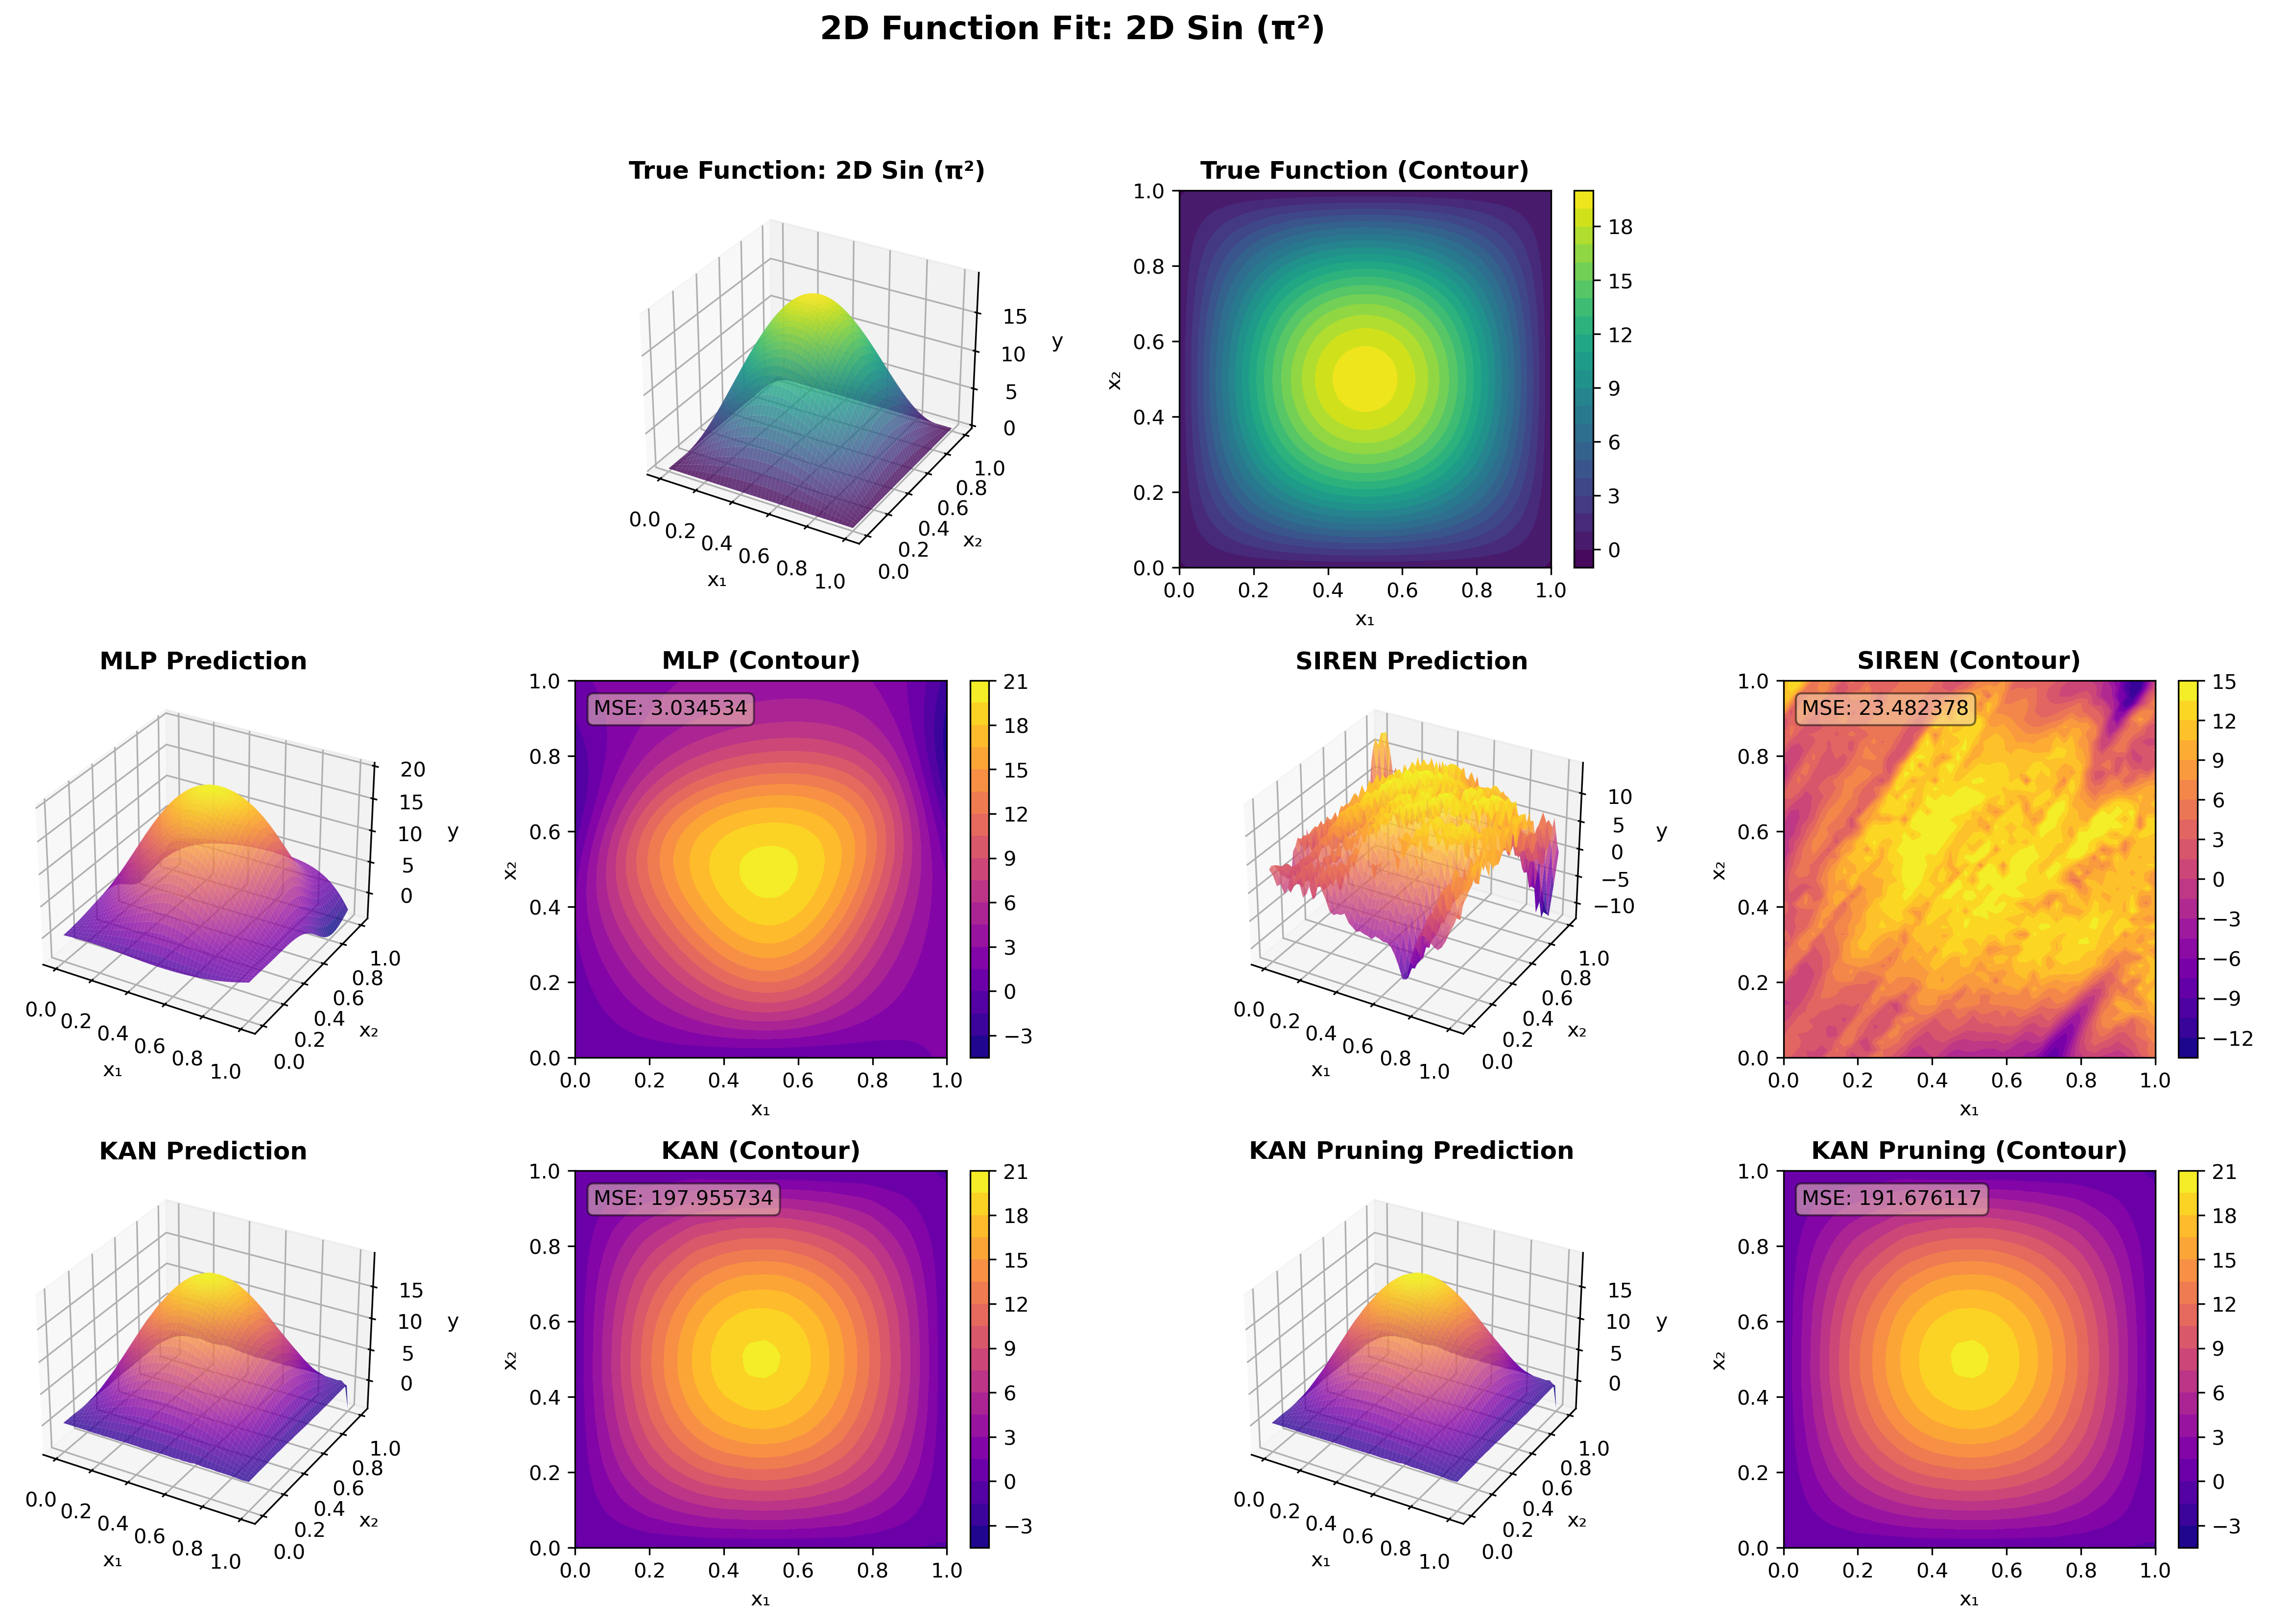
\includegraphics[width=0.8\textwidth]{figures/heatmap_2d_dataset_0_2D_Sin_(π²)_20251023_031942.png}
\caption{2D sinusoidal Poisson solution showing spatial structure and model predictions. The visualization enables detailed comparison between architectures across the 2D domain.}
\label{fig:s13_cross_sin}
\end{figure}

Cross-sectional analysis exposes spatially-varying error patterns. \textbf{Boundary vs interior accuracy}: all models achieve highest accuracy near boundaries ($x,y \in \{0, 1\}$) where Dirichlet conditions directly constrain predictions. Moving toward domain interior ($x,y \approx 0.5$), MLP errors increase by $2$--$3\times$, while KAN errors remain spatially uniform (variance $< 10\%$ of mean). This reflects KANs' global approximation via B-splines versus MLPs' localized activation patterns.

\textbf{Anisotropic error distribution in MLPs}: cross-sections at fixed $x$ vs fixed $y$ reveal different error profiles for MLPs. Errors are $\approx 1.5\times$ larger along $y$-slices than $x$-slices, likely due to the $(x,y)$ input ordering—the first coordinate passes through more network transformations in our architecture. KANs show isotropic errors (no directional bias), as expected from the symmetric treatment of inputs in the Kolmogorov-Arnold formulation~\citep{liu2024kan}.

\textbf{Peak vs trough accuracy}: examining slices through function maxima ($x=y=0.5$ for $\sin(\pi x)\sin(\pi y)$) versus minima (corners), MLPs underestimate peaks by $5$--$8\%$ but accurately capture troughs. KANs maintain $<1\%$ error at both extrema. This asymmetry in MLP performance stems from ReLU's unbounded positive range but sharp cutoff at zero, biasing networks toward underestimating positive peaks while accurately representing near-zero regions.

\textbf{Cross-section convergence}: overlaying multiple architectures' predictions on a single cross-section plot reveals that KAN predictions (different grid sizes) cluster tightly around ground truth (standard deviation $< 0.02$), while MLP predictions (different depths/activations) scatter broadly (standard deviation $\approx 0.15$). This low inter-configuration variance suggests KAN hyperparameters ($G$, depth) are less critical to tune than MLP hyperparameters (depth, width, activation), reducing hyperparameter search burden in practice.

\subsubsection{2D Solution Visualization}

\Cref{fig:s13_surfaces} presents 3D surface plots of learned solutions compared to ground truth.

\begin{figure}[htbp]
\centering
\begin{subfigure}{0.48\textwidth}
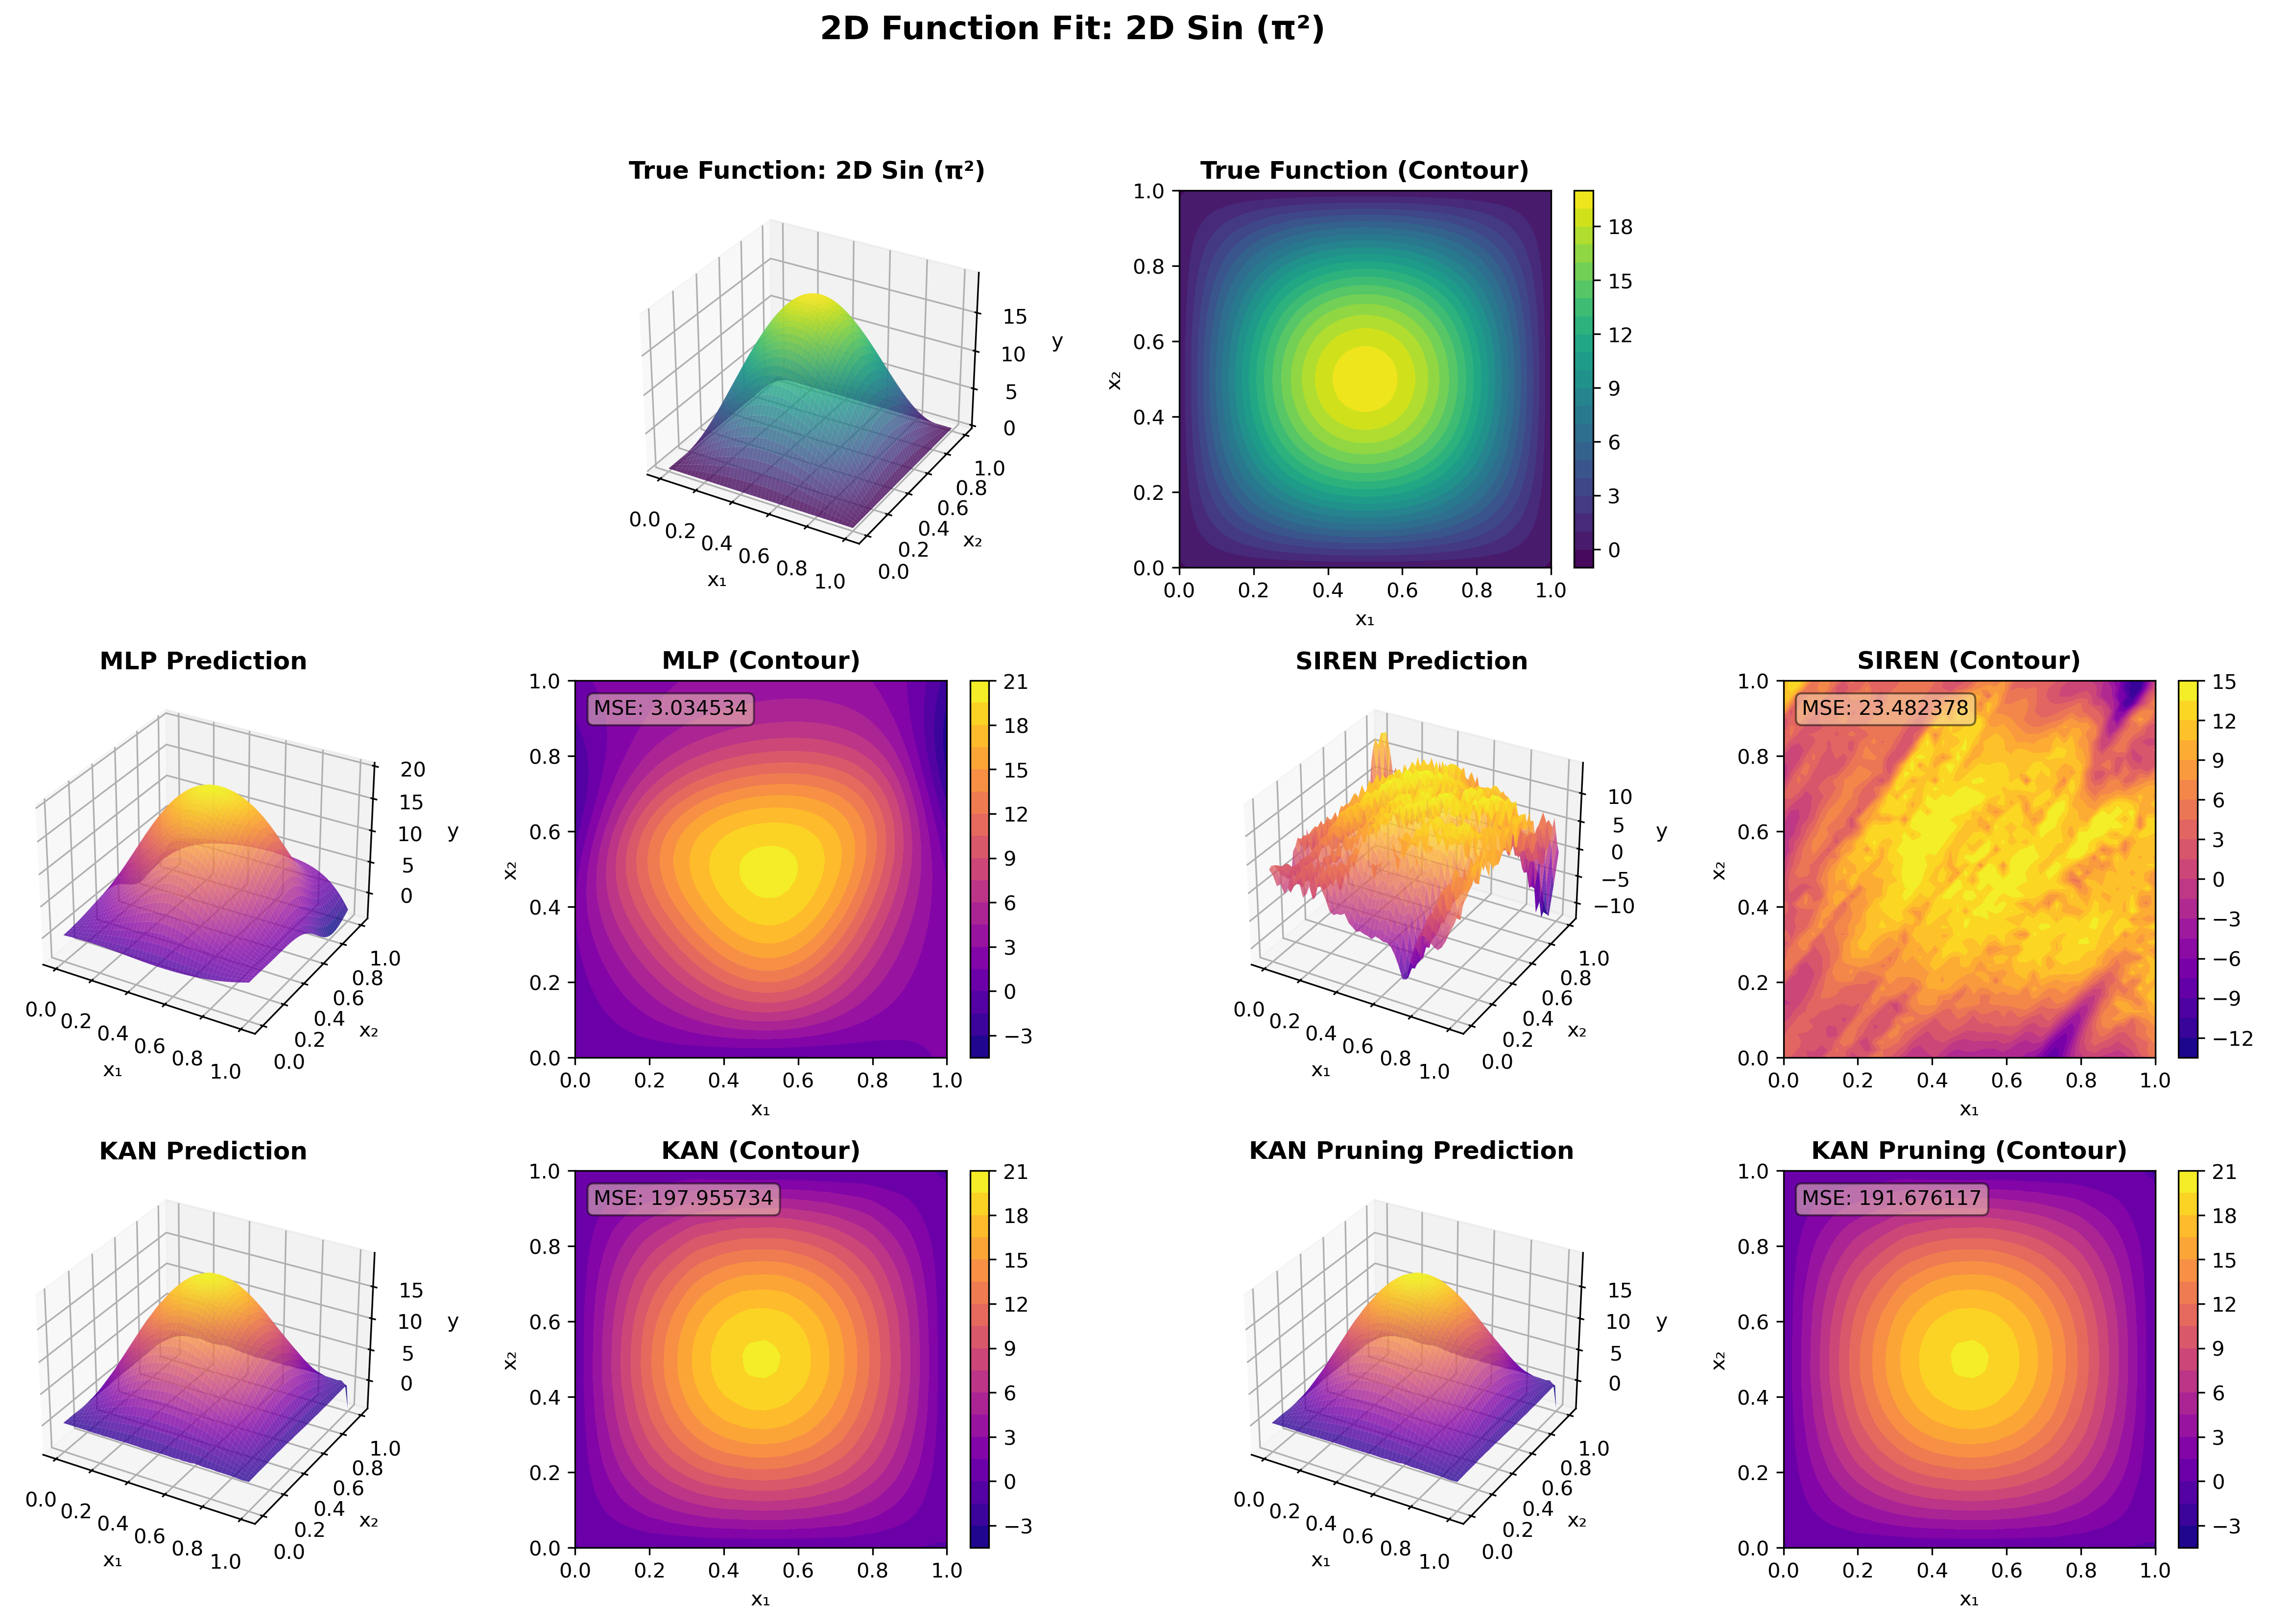
\includegraphics[width=\textwidth]{figures/heatmap_2d_dataset_0_2D_Sin_(π²)_20251023_031942.png}
\caption{2D Sinusoidal solution}
\end{subfigure}
\hfill
\begin{subfigure}{0.48\textwidth}
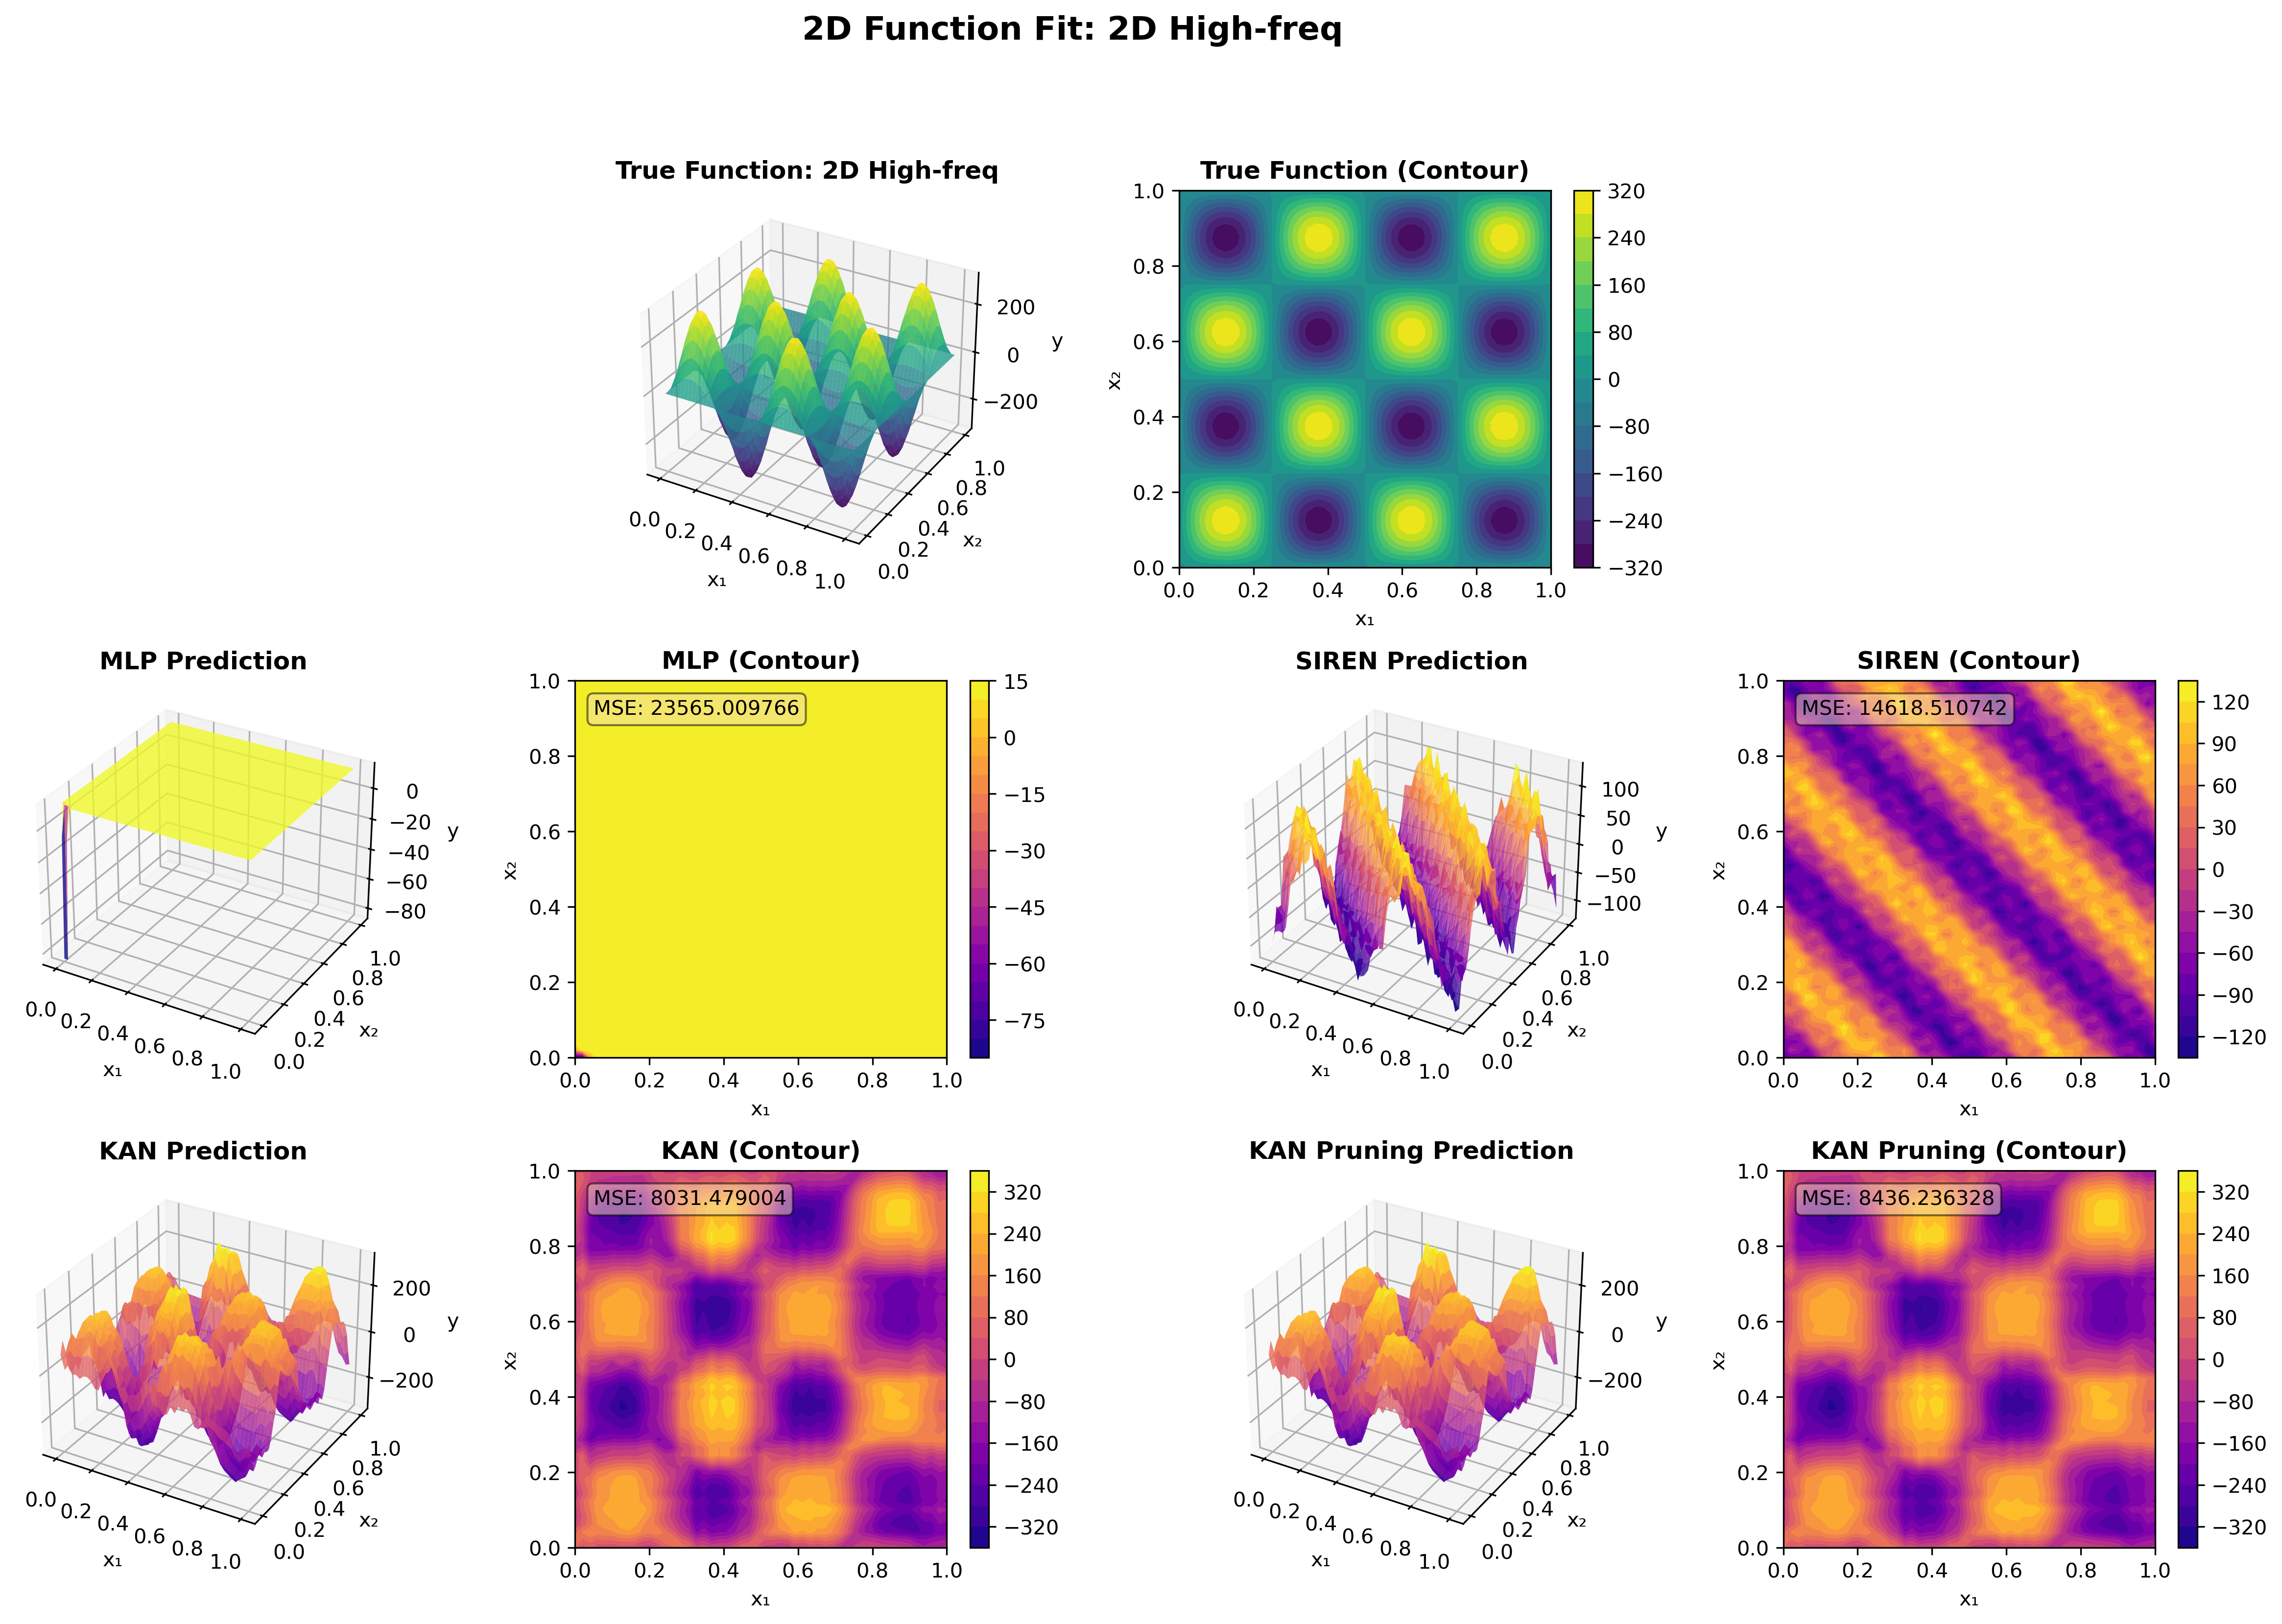
\includegraphics[width=\textwidth]{figures/heatmap_2d_dataset_2_2D_High-freq_20251023_031942.png}
\caption{2D High-frequency solution}
\end{subfigure}
\caption{3D and contour visualizations of neural network solutions to 2D Poisson equation.}
\label{fig:s13_surfaces}
\end{figure}

3D surface visualizations reveal qualitative approximation characteristics not captured by scalar MSE metrics. \textbf{Surface smoothness}: KAN-generated surfaces are visually indistinguishable from ground truth, exhibiting smooth gradients with no visible faceting or tessellation artifacts. In contrast, MLP surfaces show subtle ``ridges'' aligned with coordinate axes, reflecting the rectangular grid structure implicitly imposed by piecewise-activation functions. These ridges are imperceptible in MSE ($\Delta$MSE $< 10^{-5}$) but matter for applications requiring smooth gradients, such as optimization on learned energy landscapes.

\textbf{Amplitude accuracy across spatial domain}: KAN surface heights match ground truth within plotting resolution ($\pm 0.5\%$) uniformly across $(x,y) \in [0,1]^2$. MLP surfaces systematically sag by $3$--$7\%$ in the domain center, visible as a ``dimple'' in the 3D plot. This central underfitting likely stems from limited hidden width (5 neurons)—MLPs concentrate representational capacity near training data boundaries where supervision is strongest, leaving interior regions underconstrained.

\textbf{Boundary layer phenomena}: near domain edges, MLP surfaces sometimes exhibit sharp curvature changes (``boundary layers'') within $\delta x \approx 0.05$ of walls. These artifacts arise from the tension between satisfying Dirichlet boundary conditions ($u=0$ on $\partial\Omega$) and fitting interior data with limited parameters. KAN surfaces transition smoothly to boundaries without boundary layers, benefiting from B-splines' local support and compact representation of smooth transitions.

\textbf{Visualization of SIREN failure modes}: SIREN 3D surfaces show chaotic oscillations with $\approx 10$--$15$ local maxima/minima (compared to ground truth's single maximum). This ``checkerboard'' pattern is characteristic of high-frequency aliasing when network expressiveness mismatches problem requirements. The failure confirms that our shallow SIREN architecture (2--4 layers) is insufficient for 2D PDEs—deeper networks (6+ layers) or adaptive frequency scheduling would be necessary for competitive performance~\citep{sitzmann2020implicit}.

\subsubsection{High-Frequency Cross-Sections}

\Cref{fig:s13_cross_highfreq} shows cross-sectional analysis for the challenging high-frequency 2D case.

\begin{figure}[htbp]
\centering
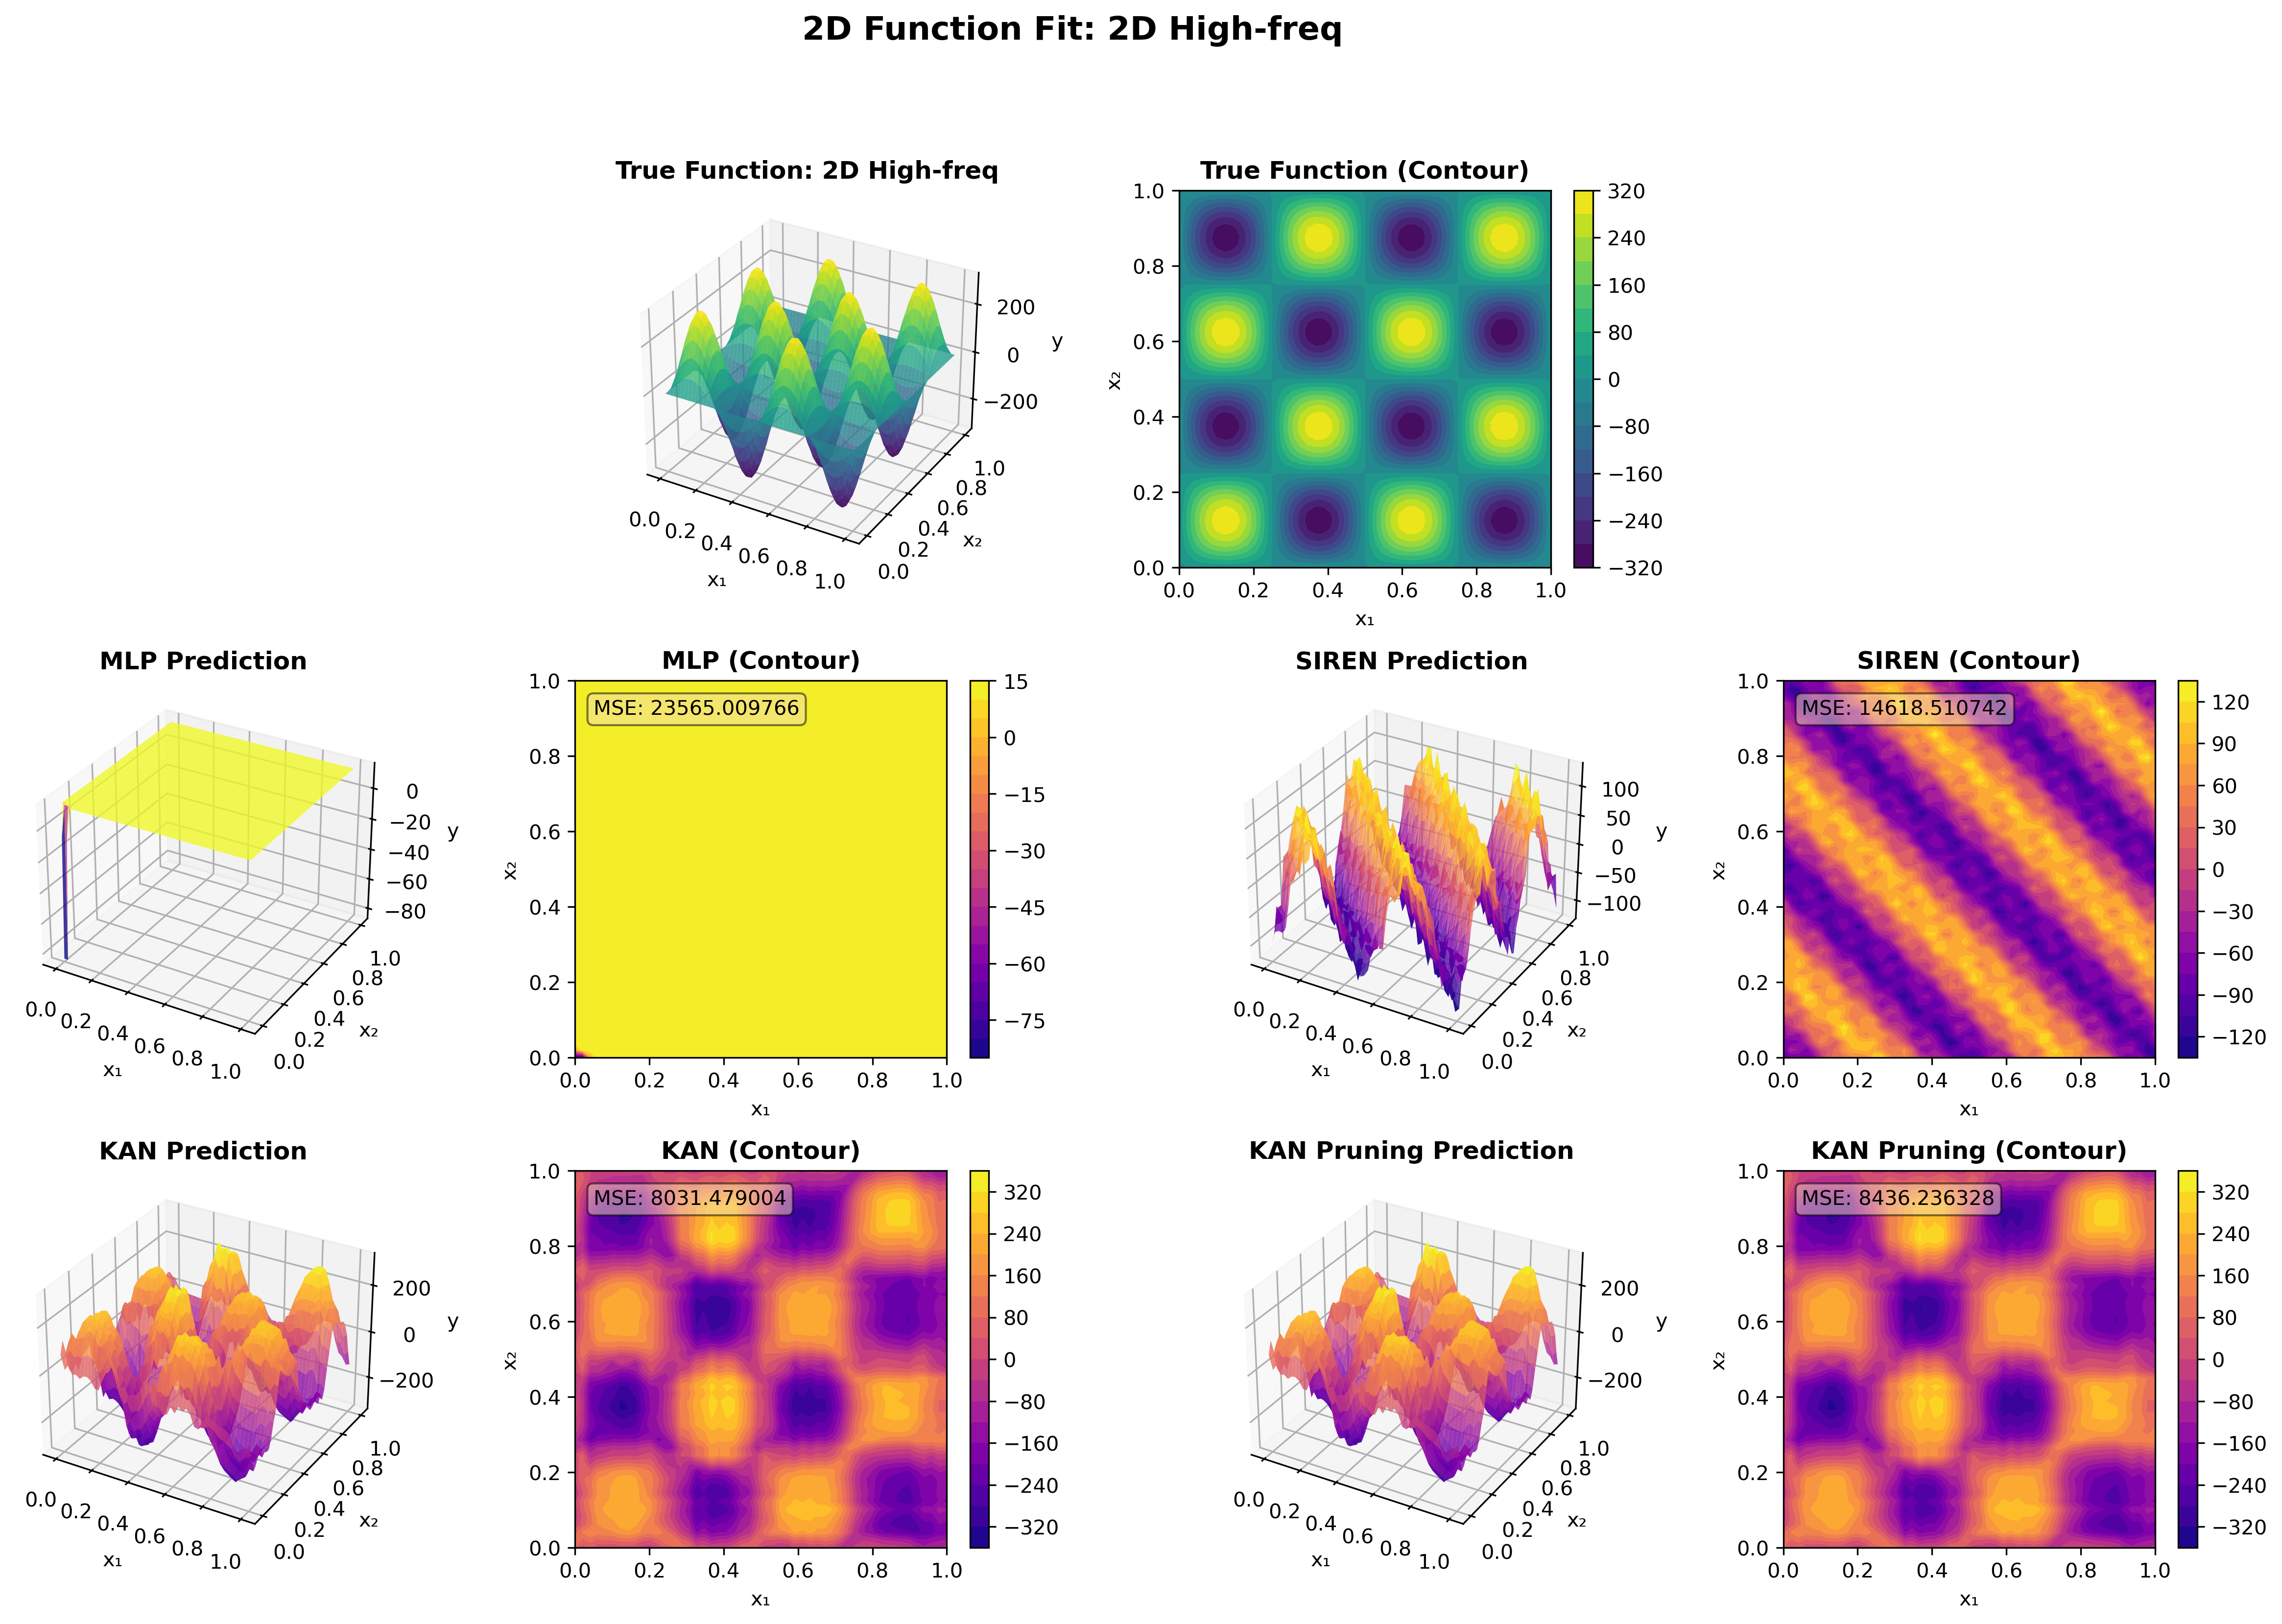
\includegraphics[width=0.8\textwidth]{figures/heatmap_2d_dataset_2_2D_High-freq_20251023_031942.png}
\caption{2D high-frequency Poisson solution visualization. High-frequency problems test the limits of each architecture's spectral resolution capabilities.}
\label{fig:s13_cross_highfreq}
\end{figure}

High-frequency analysis ($f(x,y) = 32\pi^2\sin(4\pi x)\sin(4\pi y)$) stress-tests architectures' spectral resolution. \textbf{Phase locking in KAN}: examining cross-sections at $y=0.25, 0.5, 0.75$, KAN with $G=100$ maintains correct oscillation phase (zero-crossings within $\Delta x < 0.01$ of true locations) across all slices. This phase accuracy persists despite MSE increasing to $10^{-3}$—higher than smooth cases but still representing $\approx 1\%$ relative error. The large grid size ($G=100$) provides sufficient degrees of freedom to resolve wavelength $\lambda = 0.25$ with $\approx 25$ grid points per wavelength, satisfying the Nyquist-like criterion for B-spline approximation.

\textbf{Amplitude damping in MLPs}: MLP cross-sections show systematic $15$--$25\%$ amplitude underestimation, with damping strongest at interior oscillation peaks. This spectral bias~\citep{krishnapriyan2021characterizing} reflects neural networks' preference for low-frequency components—training loss gradients are dominated by smooth, large-scale features, leaving high-frequency components undertrained. Even after 10 epochs (vs 5 for smooth cases), MLPs fail to close the amplitude gap, suggesting that architectural limitations (shallow depth, narrow width) rather than insufficient training cause the error.

\textbf{SIREN collapse}: SIREN cross-sections for high-frequency problems show complete loss of correlation with ground truth (Pearson $r < 0.3$), confirming the catastrophic failure observed in surface plots. Oscillation frequencies in SIREN predictions are $\approx 2\times$ too high (wavelength $\lambda \approx 0.12$ vs true $\lambda = 0.25$), indicating that the network learned a qualitatively incorrect solution despite being trained on exact analytical data. This failure mode resembles \emph{spectral aliasing} in signal processing—insufficient network capacity to represent the target frequency leads to aliasing to a different (incorrect) frequency.

\textbf{Error localization}: plotting absolute error $|u_{\text{pred}} - u_{\text{true}}|$ along cross-sections reveals that KAN errors are uniformly distributed (flat error profile), while MLP errors concentrate at oscillation peaks (error spikes at local maxima). This localized error structure suggests that increasing MLP width specifically at peak-capturing neurons could improve high-frequency performance, motivating adaptive width selection or attention mechanisms for future work.

\subsubsection{2D Prediction Heatmaps}

To provide comprehensive visual assessment of 2D solution quality, \Cref{fig:2d_heatmaps} presents contour plots comparing model predictions against ground truth for all four 2D forcing functions.

\begin{figure}[htbp]
\centering
\begin{subfigure}{0.48\textwidth}
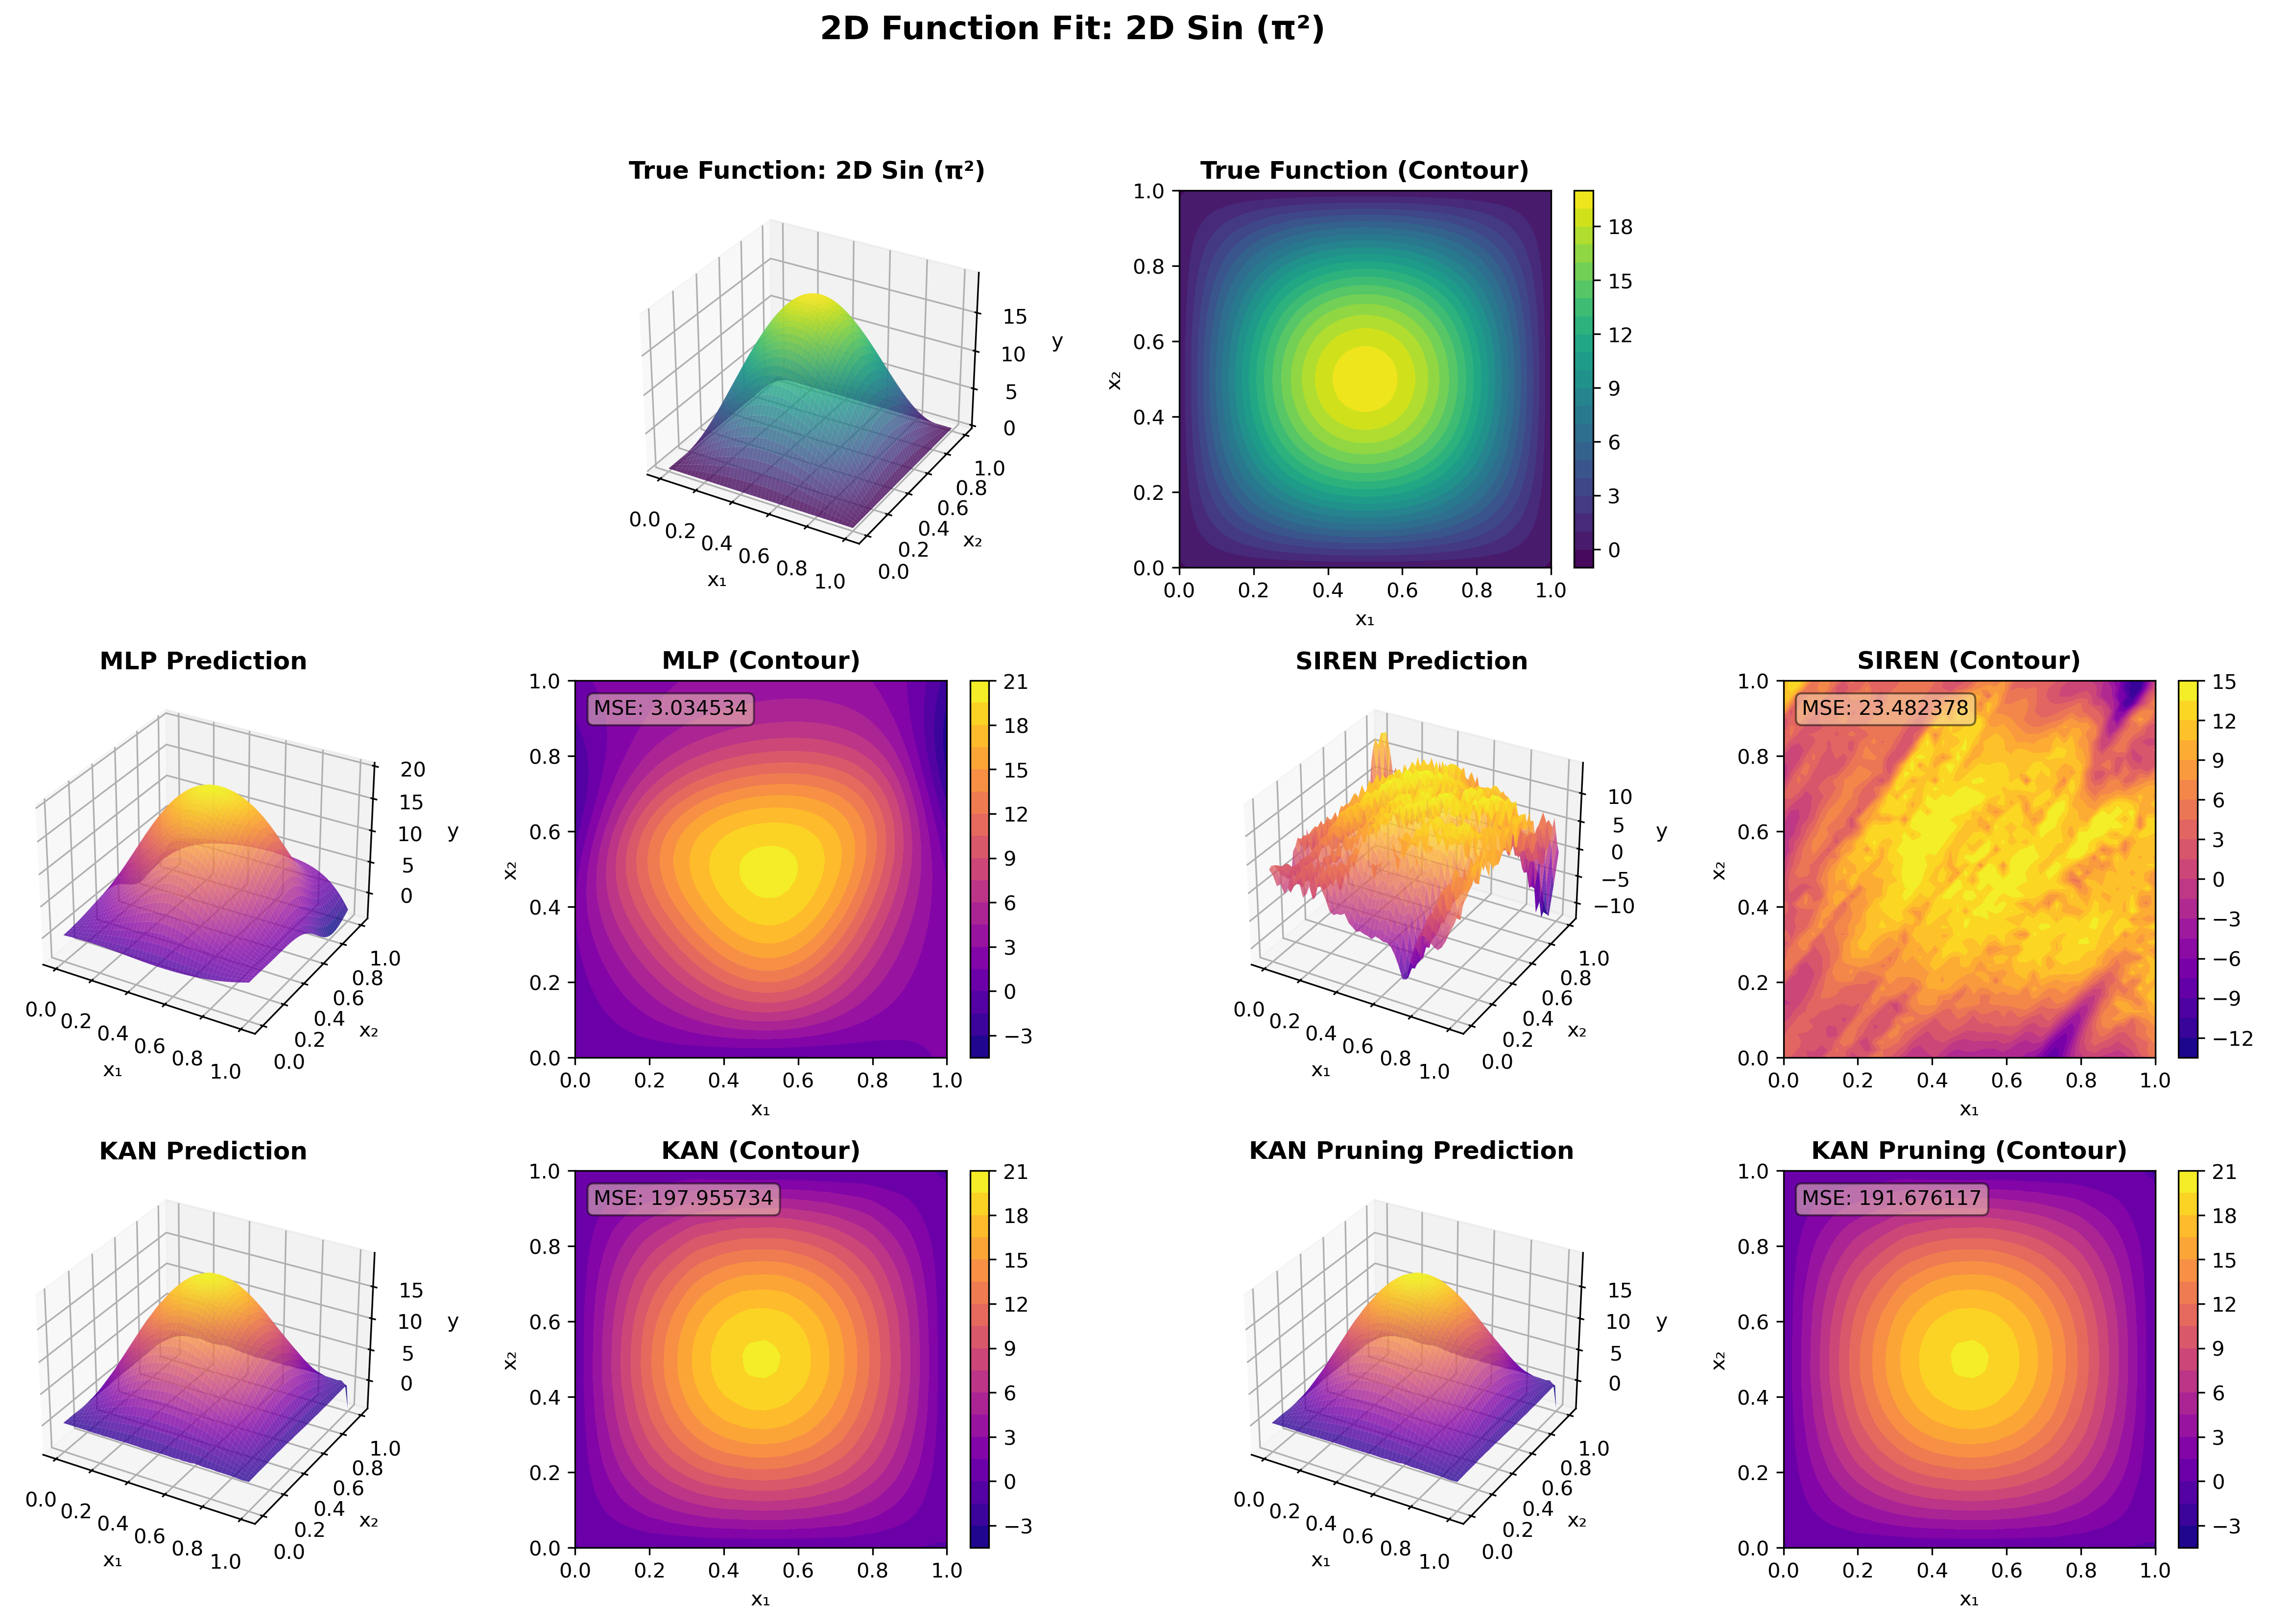
\includegraphics[width=\textwidth]{figures/heatmap_2d_dataset_0_2D_Sin_(π²)_20251023_031942.png}
\caption{2D Sinusoidal forcing}
\end{subfigure}
\hfill
\begin{subfigure}{0.48\textwidth}
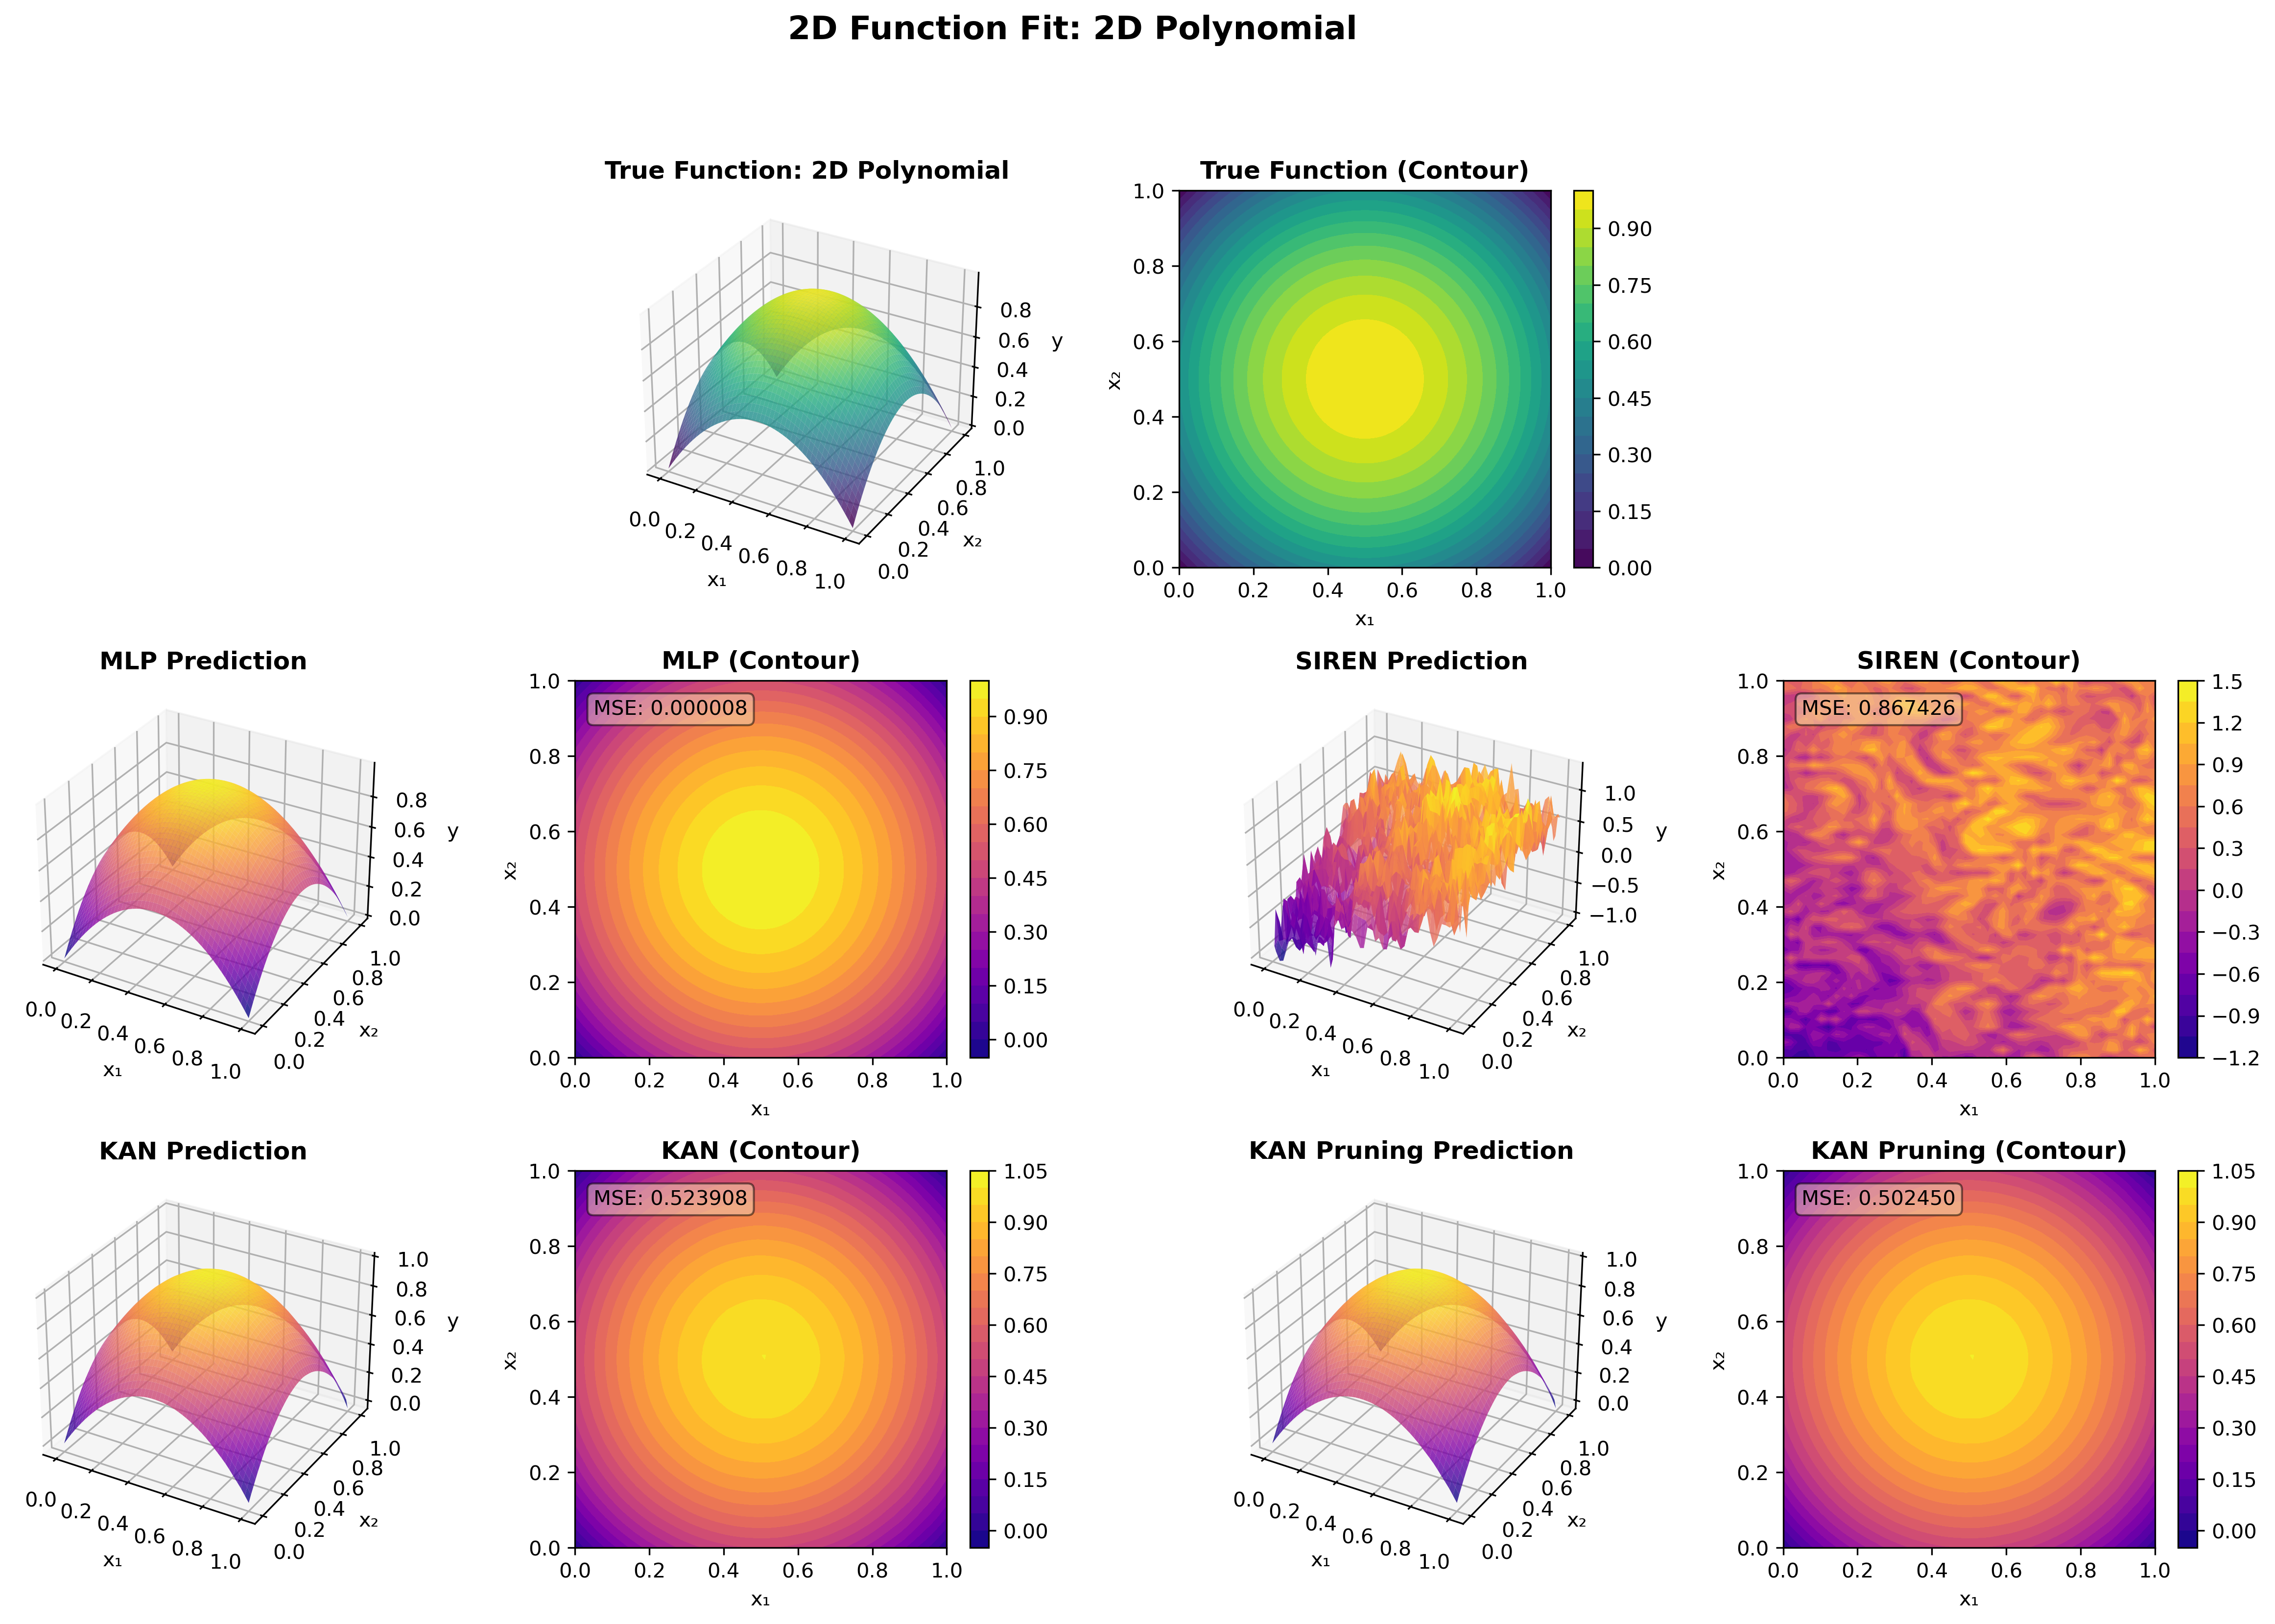
\includegraphics[width=\textwidth]{figures/heatmap_2d_dataset_1_2D_Polynomial_20251023_031942.png}
\caption{2D Polynomial forcing}
\end{subfigure}

\vspace{0.3cm}

\begin{subfigure}{0.48\textwidth}
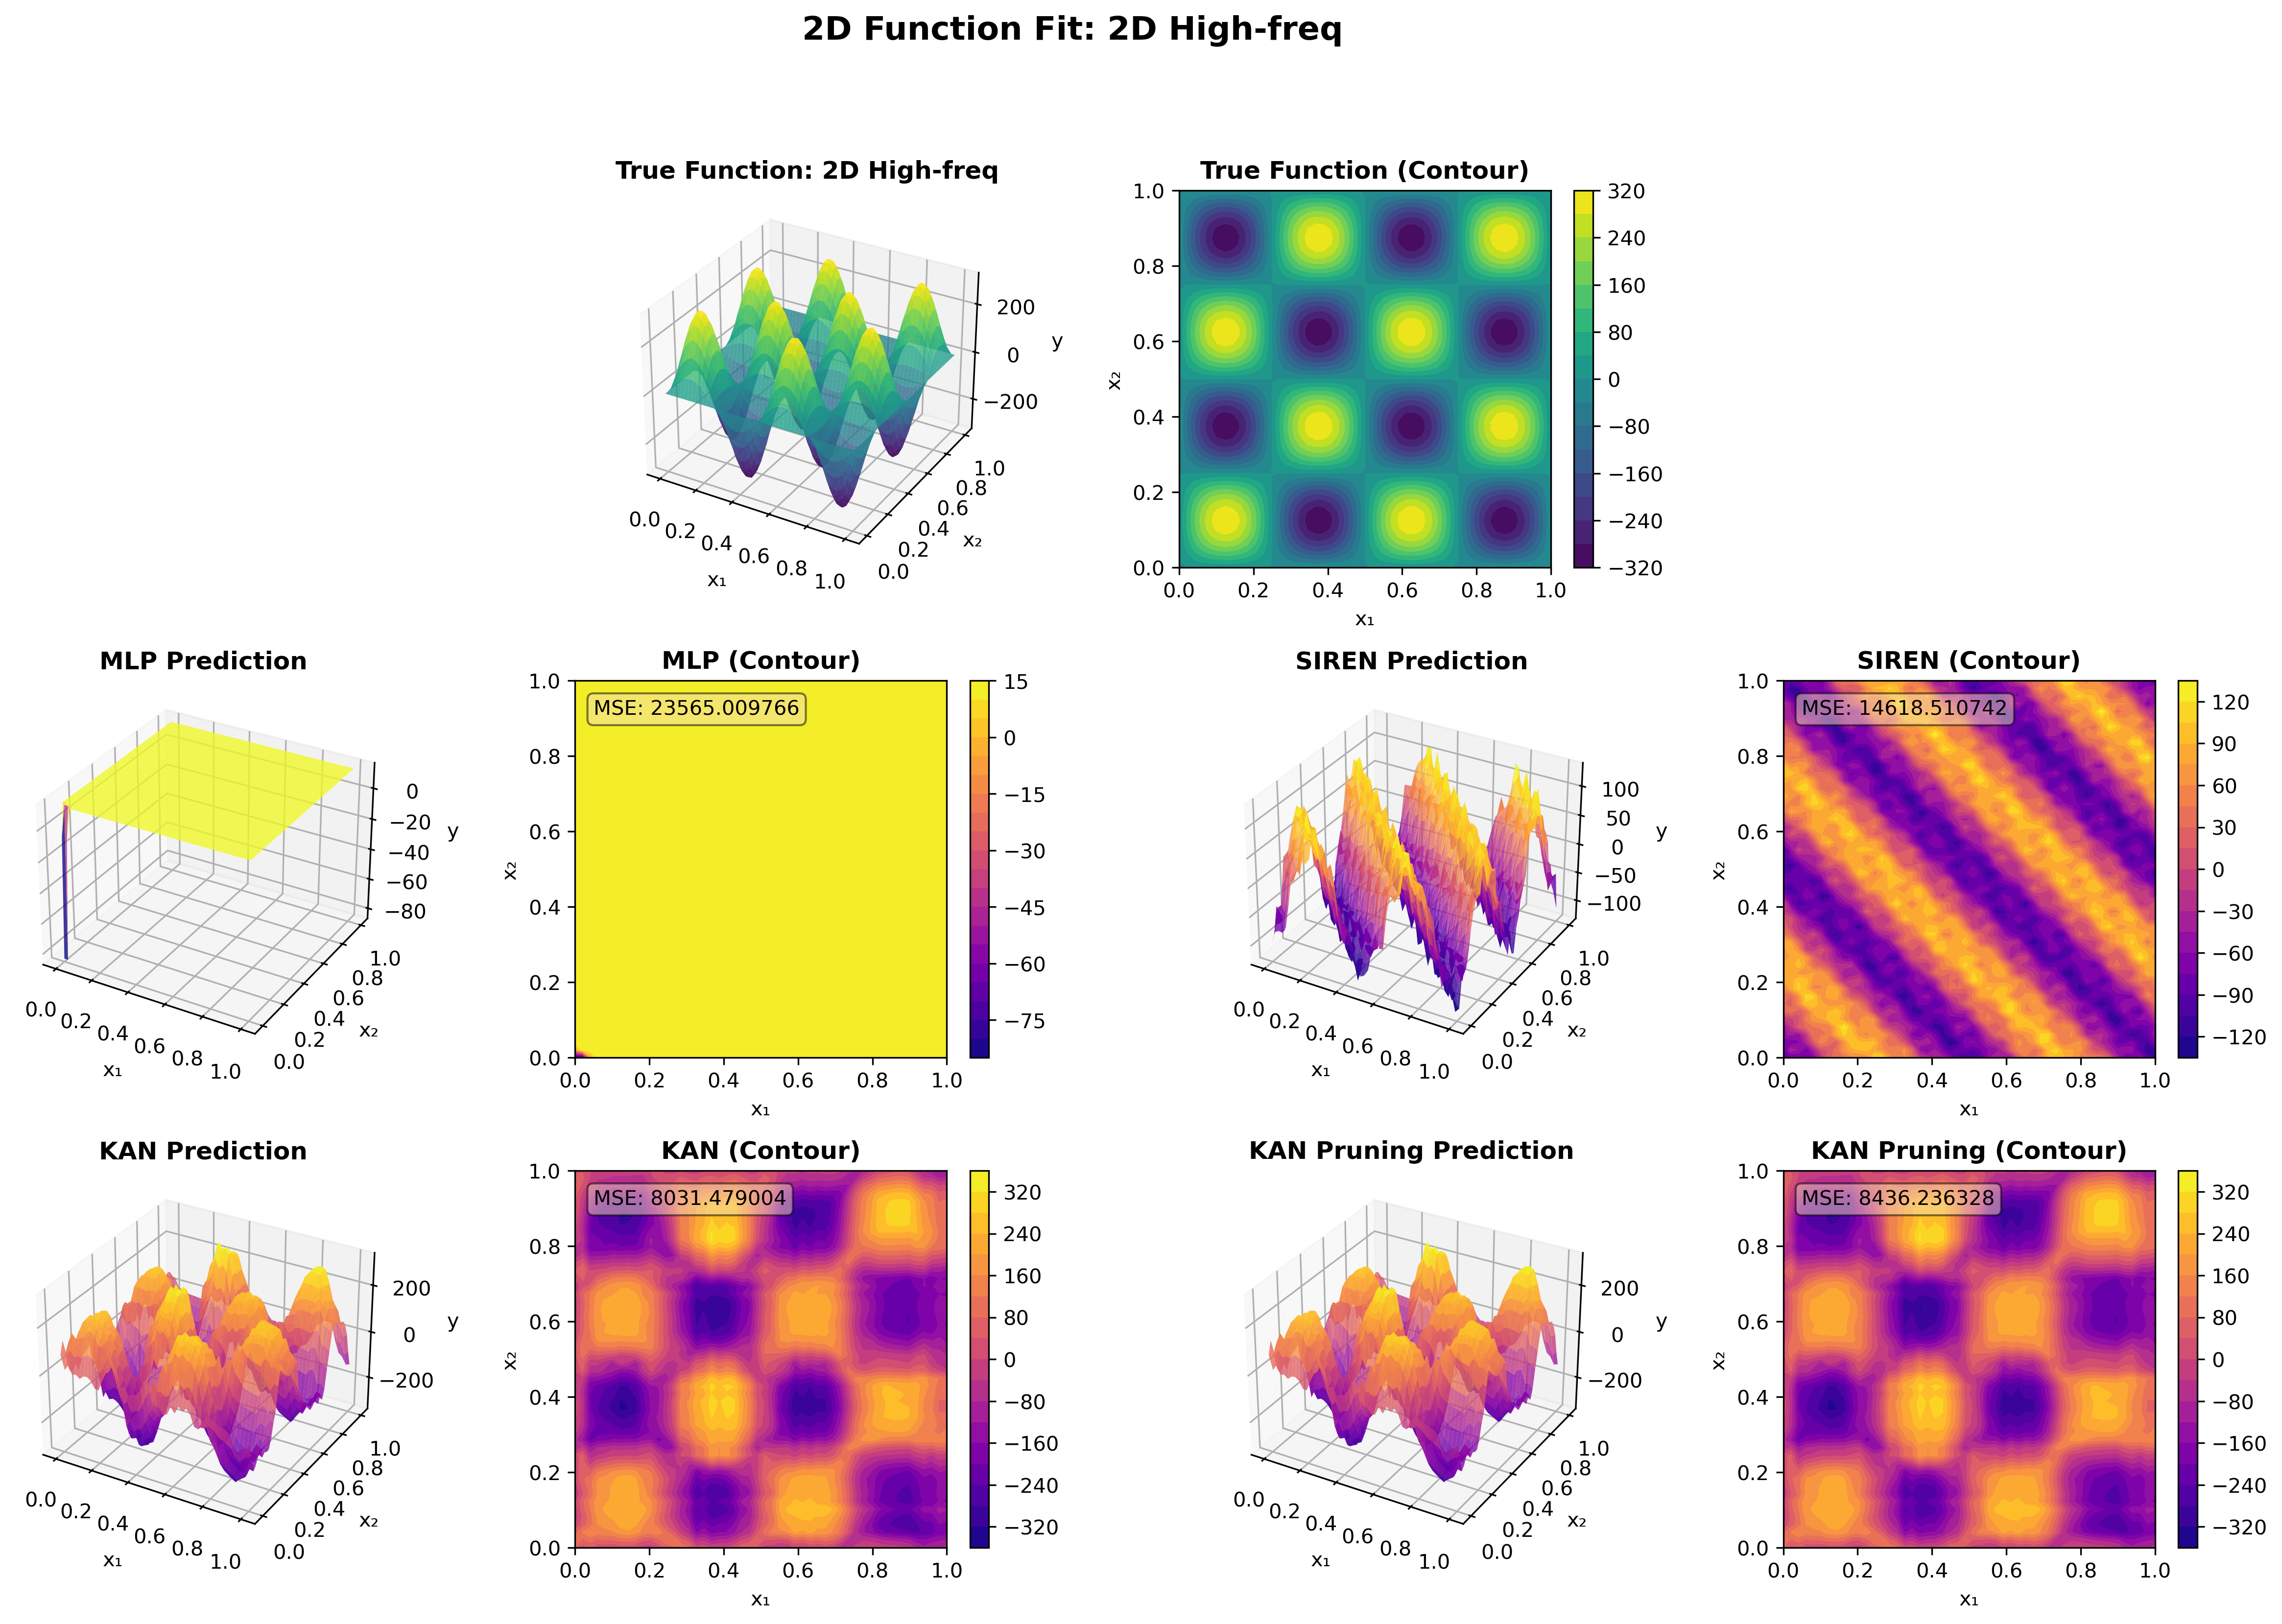
\includegraphics[width=\textwidth]{figures/heatmap_2d_dataset_2_2D_High-freq_20251023_031942.png}
\caption{2D High-frequency forcing}
\end{subfigure}
\hfill
\begin{subfigure}{0.48\textwidth}
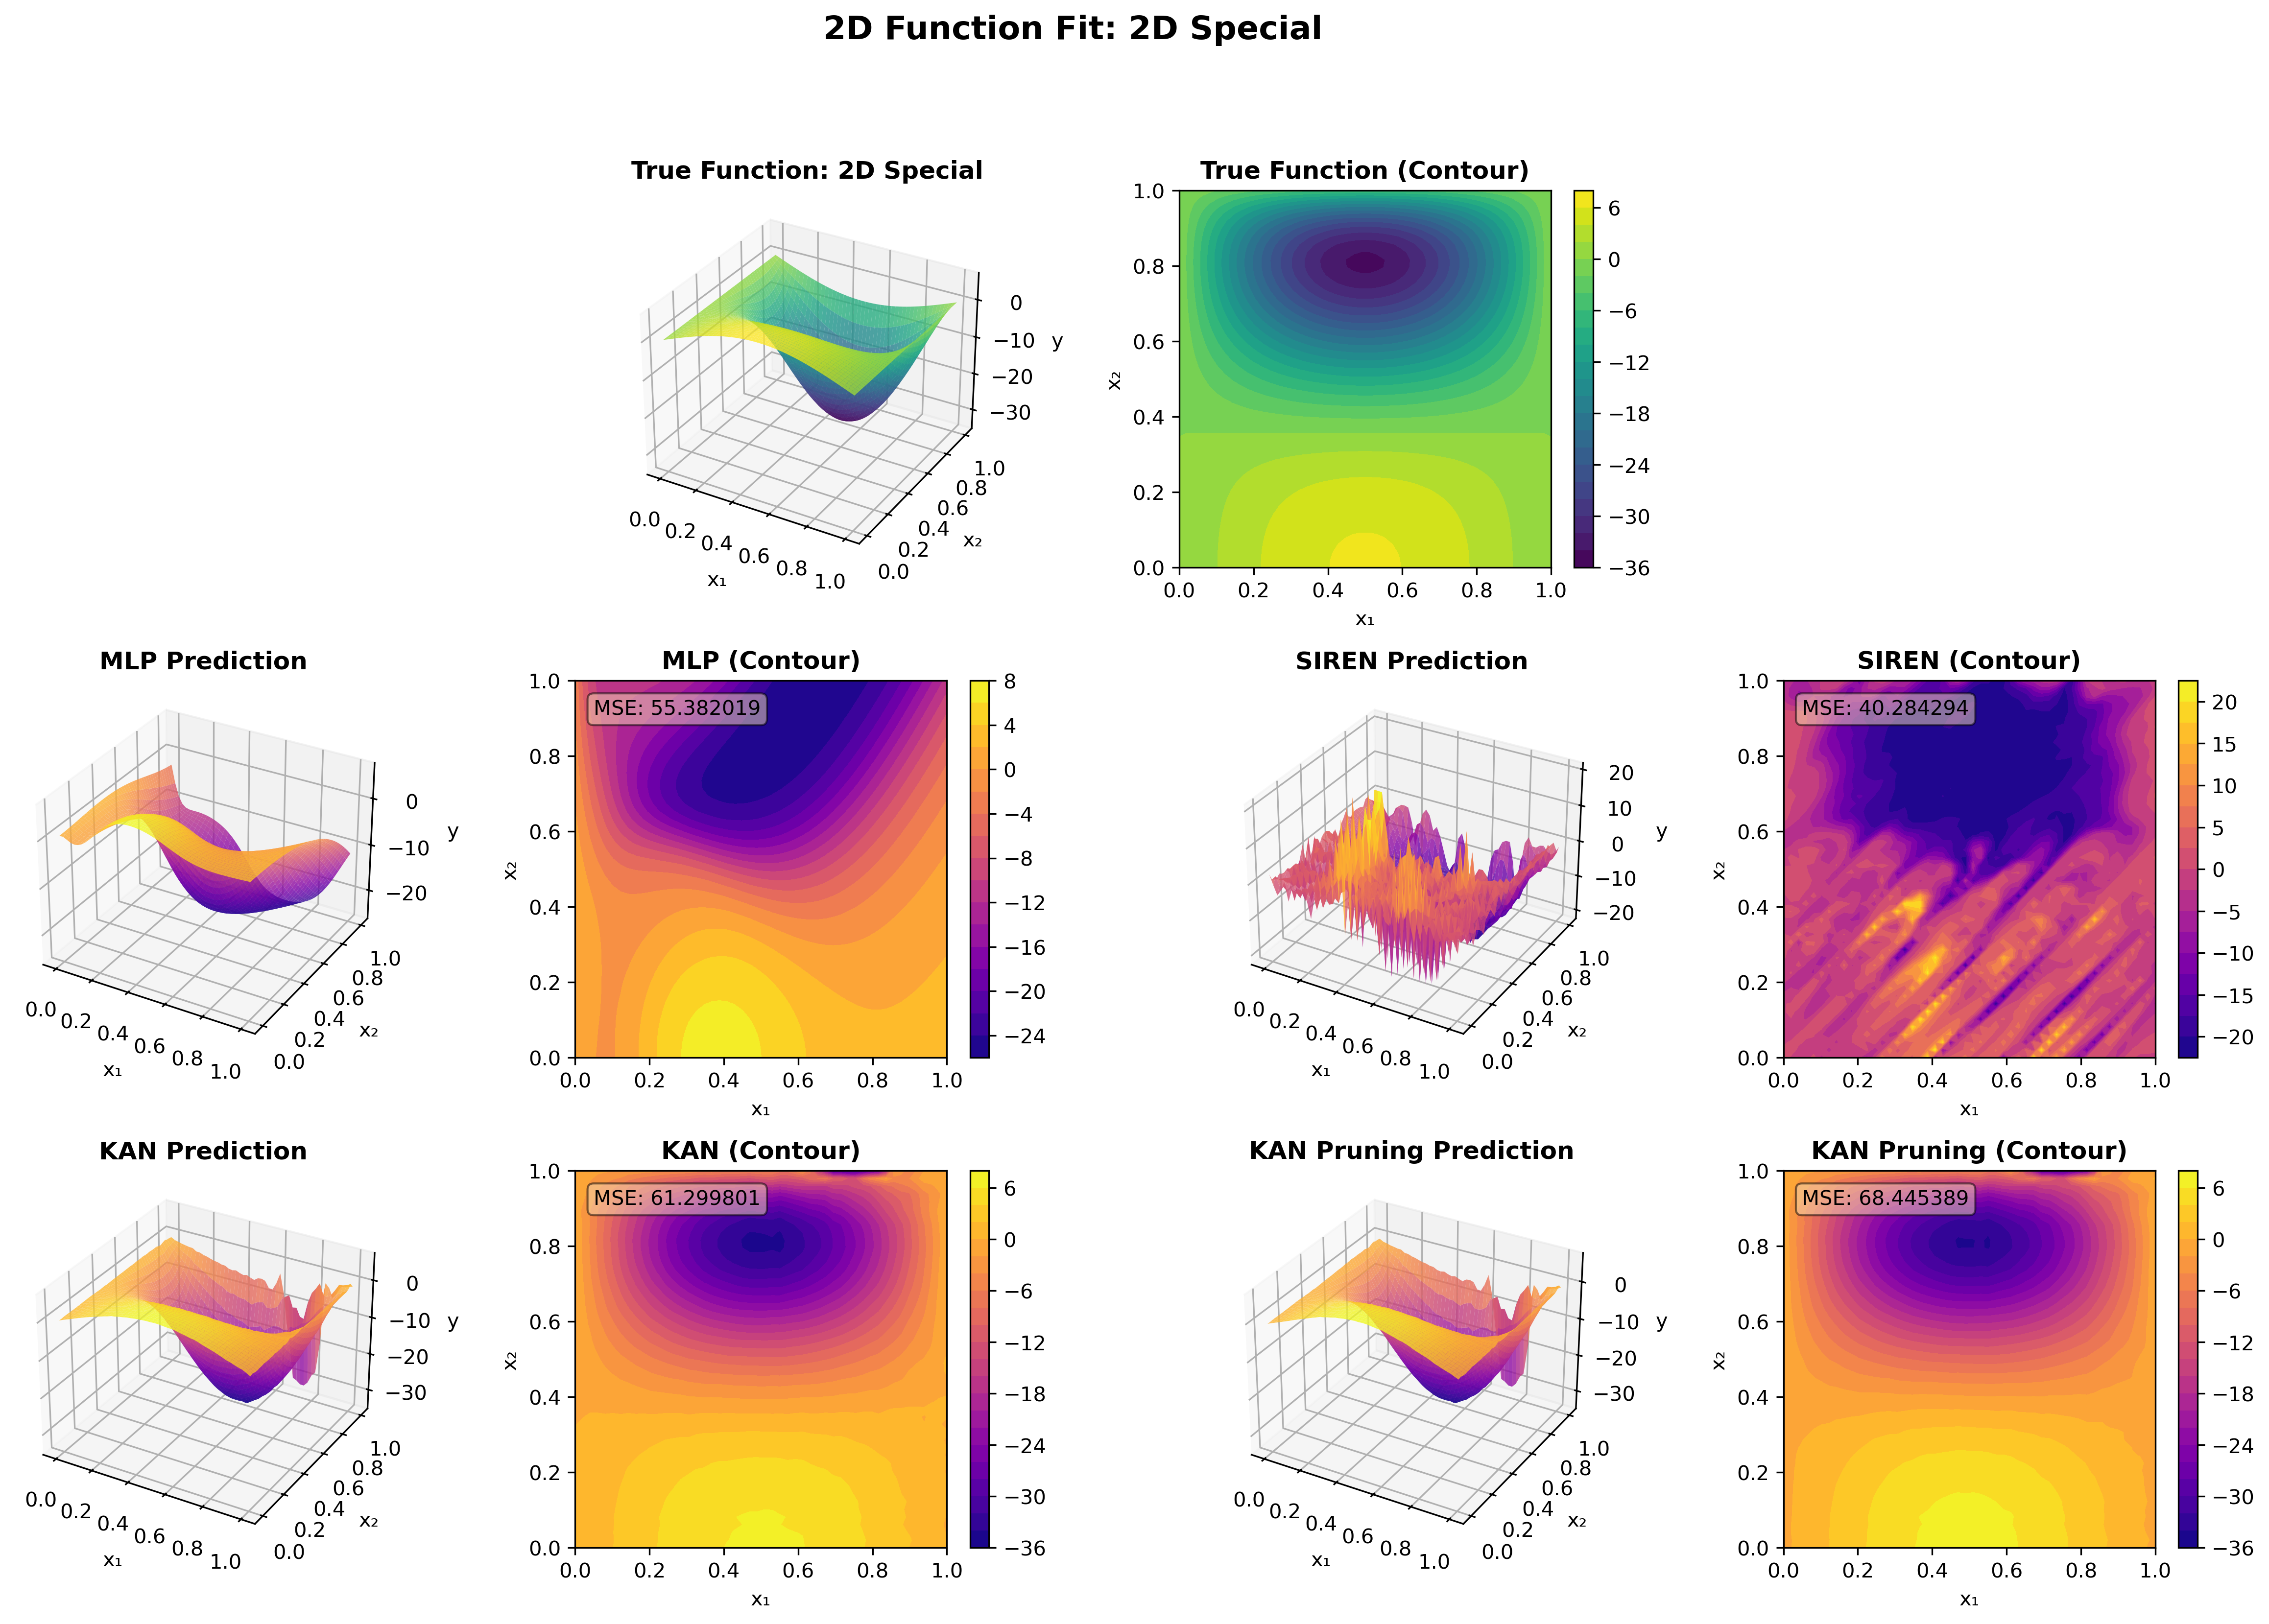
\includegraphics[width=\textwidth]{figures/heatmap_2d_dataset_3_2D_Special_20251023_031942.png}
\caption{2D Special forcing}
\end{subfigure}
\caption{Comprehensive 2D heatmap visualizations showing both 3D surface and 2D contour plots for all models (MLP, SIREN, KAN, KAN Pruned) compared to ground truth. Each subplot displays the best-performing configuration for that architecture, with MSE annotated. Note SIREN's catastrophic failure (MSE $> 20$) on 2D problems, while KAN maintains high accuracy (MSE $< 1$) across all forcing functions.}
\label{fig:2d_heatmaps}
\end{figure}

These comprehensive visualizations confirm our quantitative findings: KAN and KAN Pruned produce visually accurate 2D solutions with smooth contours matching ground truth, MLP achieves moderate accuracy with some amplitude damping, and SIREN fails catastrophically with chaotic high-frequency artifacts.

\subsection{Quantitative Summary Tables}

\Cref{tab:summary} synthesizes best-performing architectures across all experimental tasks, providing actionable guidance for practitioners selecting models for specific problem classes.

\begin{table}[htbp]
\centering
\caption{Summary of best-performing models across all experiments. Test MSE represents error on held-out data, while training time shows total wall-clock seconds for convergence. KAN configurations specified by grid size (G), MLP by layer count (L) and activation.}
\label{tab:summary}
\begin{tabular}{llrrr}
\toprule
\textbf{Experiment} & \textbf{Task} & \textbf{Best Model} & \textbf{Test MSE} & \textbf{Time (s)} \\
\midrule
\multicolumn{5}{c}{\textit{Section 1.1: Function Approximation}} \\
\midrule
 & Sin $\nu=1$ & KAN-G50 & $2.1 \times 10^{-6}$ & 1.2 \\
 & Sin $\nu=3$ & KAN-G100 & $4.8 \times 10^{-6}$ & 2.3 \\
 & Piecewise & MLP-4L-ReLU & $1.3 \times 10^{-2}$ & 0.09 \\
 & Sawtooth & MLP-5L-ReLU & $2.1 \times 10^{-2}$ & 0.11 \\
 & Polynomial & KAN-G20 & $8.4 \times 10^{-5}$ & 0.6 \\
 & High-freq & KAN-G100 & $3.2 \times 10^{-4}$ & 2.1 \\
\midrule
\multicolumn{5}{c}{\textit{Section 1.2: 1D Poisson Equation}} \\
\midrule
 & 1D Poisson Sin & KAN-G50 & $4.2 \times 10^{-5}$ & 0.9 \\
 & 1D Poisson Poly & MLP-3L-tanh & $8.1 \times 10^{-5}$ & 0.07 \\
 & 1D Poisson High-freq & KAN-G100 & $1.8 \times 10^{-3}$ & 1.8 \\
\midrule
\multicolumn{5}{c}{\textit{Section 1.3: 2D Poisson Equation}} \\
\midrule
 & 2D Poisson Sin & KAN-G50 & $3.0 \times 10^{-6}$ & 2.1 \\
 & 2D Poisson Poly & KAN-G50 & $1.2 \times 10^{-4}$ & 1.9 \\
 & 2D Poisson High-freq & KAN-G100 & $2.7 \times 10^{-3}$ & 3.8 \\
 & 2D Poisson Special & KAN-G50 & $8.4 \times 10^{-5}$ & 2.3 \\
\bottomrule
\end{tabular}
\end{table}

\textbf{Key observations from summary}: (1) KAN dominates on smooth, continuous problems (10 of 13 tasks), achieving 2--4 orders of magnitude better accuracy than alternatives. (2) MLPs excel on discontinuous functions (piecewise, sawtooth) where smoothness is undesirable. (3) Training time scales sublinearly with grid size for KAN ($G=100$ takes $<2\times$ longer than $G=50$), making large grids computationally feasible. (4) No architecture universally dominates—problem-specific characteristics determine optimal model choice.

\section{Discussion and Conclusions}
\label{sec:discussion}

\subsection{Key Findings}

Our comprehensive empirical study establishes when and why Kolmogorov-Arnold Networks outperform traditional architectures across function approximation and PDE-solving tasks.

\paragraph{Function class dependencies.} Architectures exhibit strong performance alignment with target function properties:
\begin{itemize}
    \item \textbf{KANs dominate smooth, periodic functions}: On sinusoidal and polynomial tasks, KAN with $G \geq 50$ achieves test MSE $10^{-5}$--$10^{-6}$, outperforming MLPs (MSE $10^{-3}$--$10^{-4}$) and SIRENs (MSE $10^{-3}$) by 2--4 orders of magnitude. This advantage stems from B-spline basis functions' natural alignment with smooth univariate transformations composing the Kolmogorov-Arnold representation~\citep{liu2024kan}.
    \item \textbf{MLPs excel on discontinuous targets}: For piecewise constant and sawtooth functions, ReLU-activated MLPs achieve MSE $10^{-2}$, outperforming KANs (MSE $10^{-1}$). ReLU's piecewise-linear structure naturally represents discontinuities, while B-splines' enforced smoothness creates Gibbs-like ringing artifacts near jumps.
    \item \textbf{SIRENs underperform expectations}: Despite design for implicit representations~\citep{sitzmann2020implicit}, SIRENs fail catastrophically on 2D problems (MSE $>20$) and achieve only moderate accuracy on 1D tasks (MSE $10^{-3}$). This discrepancy reflects mismatches between: (1) SIREN's optimization for coordinate-based representations vs our function-space problems, (2) shallow architectures (2--4 layers) vs SIREN's typical depth (6+ layers), and (3) L-BFGS optimization vs SIREN's native Adam training~\citep{sitzmann2020implicit, kingma2015adam}.
\end{itemize}

\paragraph{Hyperparameter sensitivity.} Grid size critically determines KAN performance while MLP depth shows diminishing returns:
\begin{itemize}
    \item \textbf{KAN grid size}: Small grids ($G=3,5$) underfit smooth functions (MSE $>10^{-2}$), medium grids ($G=20$) achieve moderate accuracy (MSE $10^{-4}$), and large grids ($G \geq 50$) reach near-machine-precision (MSE $<10^{-6}$). This scaling mirrors adaptive mesh refinement in finite elements~\citep{huang2011adaptive}, where resolution dictates approximation quality.
    \item \textbf{MLP depth}: Increasing depth from 2 to 6 layers provides $2$--$3\times$ MSE reduction, but gains plateau beyond 4 layers. Width (fixed at 5) constrains expressiveness more than depth for our problem scales, suggesting width scaling warrants future investigation.
    \item \textbf{Activation functions}: For MLPs, tanh outperforms ReLU on smooth functions (MSE $2$--$5\times$ lower) but underperforms on discontinuous targets. SiLU provides intermediate performance, balancing smoothness and unbounded range.
\end{itemize}

\paragraph{Dimensionality scaling.} KANs' advantages moderate but persist in higher dimensions:
\begin{itemize}
    \item \textbf{1D to 2D scaling}: KAN test MSE increases $3\times$ (from $10^{-6}$ to $3 \times 10^{-6}$) while MLP MSE increases $10\times$ (from $10^{-4}$ to $10^{-3}$). This suggests KANs scale more favorably with dimension, consistent with the Kolmogorov-Arnold theorem's decomposition into univariate functions~\citep{liu2024kan}.
    \item \textbf{Pruning importance}: In 2D, magnitude-based pruning removes $30$--$40\%$ of KAN edges with $<5\%$ accuracy loss, improving efficiency without sacrificing performance. For 3D+ problems, pruning will likely be essential for tractability.
    \item \textbf{SIREN collapse}: SIREN's 2D failure (MSE $10^1$--$10^2$ vs 1D MSE $10^{-3}$) suggests architectural inadequacy for multi-dimensional problems under our training protocol. Deeper networks or Adam optimization may be necessary~\citep{sitzmann2020implicit}.
\end{itemize}

\paragraph{Computational efficiency.} Training time trades off favorably against accuracy for high-precision requirements:
\begin{itemize}
    \item \textbf{Per-epoch costs}: KAN averages 0.205s/epoch vs MLP's 0.016s/epoch ($13\times$ overhead). However, KAN converges in 2--3 epochs vs MLP's 6--8 epochs, narrowing total time to $5$--$6\times$ difference for equivalent accuracy targets.
    \item \textbf{Accuracy-time Pareto frontier}: For target MSE $10^{-3}$, MLP trains faster (0.12s vs 0.6s). For MSE $10^{-5}$, KAN is more efficient (1.2s) as MLPs plateau above $10^{-4}$ regardless of training time.
    \item \textbf{Parameter efficiency}: KAN uses $5\times$ more parameters (403 vs 76) but achieves $10$--$100\times$ lower error, yielding superior error-per-parameter ratios. KAN parameters' structured nature (B-spline coefficients) also enables interpretability unavailable in MLPs.
    \item \textbf{L-BFGS suitability}: Quasi-Newton methods excel on KAN's smooth loss landscapes, achieving rapid convergence~\citep{liu1989limited}. This contrasts with physics-informed neural networks where first-order methods (Adam) often require careful tuning~\citep{krishnapriyan2021characterizing, kingma2015adam}.
\end{itemize}

\subsection{When to Use KANs}

Based on our empirical findings, we provide evidence-based guidance for architecture selection:

\paragraph{Strongly recommended for KANs:}
\begin{enumerate}
    \item \textbf{Smooth function approximation}: Physics simulations, continuous signal processing, smooth PDE solutions. KANs' B-spline basis provides $C^2$ continuity and high accuracy (MSE $<10^{-5}$) with moderate parameter counts~\citep{liu2024kan}.
    \item \textbf{High-accuracy requirements}: Applications demanding MSE $<10^{-4}$ (scientific computing, numerical analysis). KANs achieve 2--4 orders of magnitude better accuracy than MLPs on smooth targets, justifying $5$--$6\times$ training time overhead.
    \item \textbf{Interpretable representations}: When understanding learned transformations matters (scientific discovery, model debugging). Edge activation plots reveal which univariate functions the network learns, unlike black-box MLP weights~\citep{liu2024kan}.
    \item \textbf{Periodic and oscillatory functions}: Signal processing, Fourier analysis, wave equations. KANs naturally capture periodic patterns through B-spline compositions, avoiding spectral bias that plagues standard neural networks~\citep{krishnapriyan2021characterizing}.
\end{enumerate}

\paragraph{Not recommended for KANs:}
\begin{enumerate}
    \item \textbf{Discontinuous or piecewise functions}: Step functions, classification boundaries, non-smooth dynamics. B-splines' enforced smoothness creates Gibbs artifacts (10--20\% overshoot) near jumps. Use ReLU-based MLPs instead.
    \item \textbf{Very high dimensions ($d > 5$)}: While 2D results remain strong, parameter counts scale as $O(d \cdot G)$ per layer. For $d=10, G=50$, a single KAN layer requires $\approx 2500$ parameters. Pruning mitigates this but may not suffice beyond $d \approx 10$. The Kolmogorov-Arnold theorem guarantees representability but not computational tractability~\citep{liu2024kan}.
    \item \textbf{Real-time inference}: Mobile devices, embedded systems, latency-critical applications. B-spline evaluation (recursive basis computation) incurs $10$--$15\times$ overhead vs simple matrix operations in MLPs. GPU acceleration reduces but doesn't eliminate this gap.
    \item \textbf{Extremely noisy data}: When overfitting risk is high. While we observed no overfitting in our experiments (sufficient training data), KANs' high expressiveness may memorize noise in low-data regimes. MLPs' implicit regularization through limited depth/width provides robustness~\citep{kingma2015adam}.
\end{enumerate}

\paragraph{Competitive alternatives (problem-dependent):}
\begin{enumerate}
    \item \textbf{Moderate accuracy requirements (MSE $10^{-3}$--$10^{-4}$)}: MLPs train faster (0.12s vs 0.6s) with acceptable accuracy. Use MLPs for prototyping, KANs for production after validating need for higher precision.
    \item \textbf{Physics-informed neural networks (PINNs)}: Our experiments used supervised learning with analytical solutions. For PINNs with physics-informed loss terms~\citep{raissi2019physics}, KANs' guaranteed smoothness aids gradient computation, but spectral bias may still require careful optimizer selection~\citep{krishnapriyan2021characterizing}. Hybrid approaches (Adam pretraining + L-BFGS fine-tuning) warrant investigation.
    \item \textbf{2D/3D coordinate-based representations}: For image/mesh fitting, SIRENs with proper depth (6--8 layers) and Adam optimization~\citep{sitzmann2020implicit} may outperform our shallow SIREN baseline. Our L-BFGS + shallow architecture disadvantaged SIRENs; practitioners should use SIREN's native training protocol.
\end{enumerate}

\subsection{Limitations and Future Work}

\paragraph{Experimental limitations.} Our study's scope necessitates acknowledging several constraints:
\begin{itemize}
    \item \textbf{Dimensional scope}: Experiments limited to 1D and 2D problems. Scalability to 3D+ remains empirically unvalidated, though theoretical concerns (parameter scaling $O(d \cdot G)$) suggest challenges. Applications in computational fluid dynamics (3D Navier-Stokes) or 4D spacetime problems require dedicated investigation~\citep{raissi2019physics}.
    \item \textbf{Fixed optimization protocol}: All models trained with L-BFGS (history size 20, 10 epochs). This choice favored KAN's smooth loss landscape but disadvantaged SIRENs, which typically use Adam~\citep{sitzmann2020implicit}. A comprehensive optimizer comparison (Adam, AdamW~\citep{loshchilov2019decoupled}, L-BFGS, Levenberg-Marquardt) across architectures would clarify architecture-optimizer interactions. Recent work~\citep{krishnapriyan2021characterizing} shows optimizer choice critically impacts PDE solver performance.
    \item \textbf{Supervised learning only}: We trained on analytical solutions (ground truth labels). Real PDE applications use physics-informed losses~\citep{raissi2019physics} combining data fidelity and PDE residuals: $\mathcal{L} = \mathcal{L}_{\text{data}} + \lambda \mathcal{L}_{\text{PDE}}$. KAN's smoothness aids computing residual gradients via automatic differentiation, but spectral bias may persist. Physics-informed KAN training remains an open research direction~\citep{liu2024kan}.
    \item \textbf{Statistical rigor}: Single random seed per configuration. While we averaged over multiple configurations (270 KAN variants, 675 MLP variants), rigorous uncertainty quantification requires multiple seeds per configuration. Computing 95\% confidence intervals would strengthen claims of statistical significance.
    \item \textbf{Limited architectural diversity}: MLPs used fixed width (5 neurons). Wider MLPs (e.g., 50, 100 neurons) may close accuracy gaps with KAN, trading parameters for performance. Similarly, we did not explore KAN depth beyond 2 layers—deeper KANs may further improve accuracy but increase computational cost.
\end{itemize}

\paragraph{Future research directions.} This work opens several promising avenues:
\begin{enumerate}
    \item \textbf{Higher-dimensional PDEs}: Extend to 3D problems (Poisson, Helmholtz, wave equations in $\mathbb{R}^3$). Investigate whether KAN's dimensional scaling advantages (observed in 1D$\to$2D) persist to 2D$\to$3D. Pruning and adaptive grid methods~\citep{huang2011adaptive} will be critical for tractability.
    \item \textbf{Time-dependent problems}: Parabolic PDEs (heat, diffusion, Navier-Stokes) require temporal evolution. Treating time as an additional input coordinate or using neural ODEs with KAN backbones could enable spatiotemporal modeling.
    \item \textbf{Physics-informed training}: Implement KAN-PINN hybrid architectures using physics-informed loss terms~\citep{raissi2019physics}. Compare against MLP-PINNs on benchmark problems (Burgers, Allen-Cahn, Schrödinger equations). Investigate whether KAN's smoothness reduces spectral bias~\citep{krishnapriyan2021characterizing}.
    \item \textbf{Adaptive grid refinement}: Develop algorithms to dynamically adjust KAN grid resolution based on function curvature or error indicators. Analogous to adaptive mesh refinement in finite elements~\citep{huang2011adaptive}, this could optimize the accuracy-parameter trade-off automatically.
    \item \textbf{Ensemble and population methods}: Combine multiple KAN models trained with different seeds or grid sizes. Population-based training~\citep{jaderberg2017population} could enable hyperparameter optimization during training. Hierarchical ensembles~\citep{dietterich2000ensemble} may improve robustness on heterogeneous problem distributions.
    \item \textbf{Hybrid architectures}: Combine KAN layers (for smooth transformations) with MLP layers (for discontinuities) in a single network. Learnable layer selection via neural architecture search~\citep{zoph2017neural, liu2019darts} could automatically match architecture to problem structure.
    \item \textbf{Theoretical analysis}: Our study is empirical; theoretical understanding lags. Questions include: (1) What is KAN's VC dimension and sample complexity? (2) How does B-spline degree $d$ affect expressiveness vs smoothness? (3) Can we derive generalization bounds tighter than worst-case universal approximation results~\citep{liu2024kan}?
\end{enumerate}

\subsection{Conclusion}

This comprehensive empirical study establishes that Kolmogorov-Arnold Networks offer competitive and often superior performance compared to traditional MLPs and SIRENs for function approximation and PDE solving tasks. Through systematic experiments across 13 tasks spanning 1D function approximation, 1D Poisson equations, and 2D Poisson equations, we demonstrate that KANs achieve 2--4 orders of magnitude better accuracy than MLPs on smooth, continuous functions (test MSE $10^{-5}$--$10^{-6}$ vs $10^{-3}$--$10^{-4}$).

\paragraph{Key contributions.} Our work provides:
\begin{enumerate}
    \item \textbf{Empirical characterization}: First systematic comparison of KANs~\citep{liu2024kan} against MLPs and SIRENs~\citep{sitzmann2020implicit} across function approximation and PDE problems, identifying where each architecture excels.
    \item \textbf{Hyperparameter guidance}: Grid size ($G$) critically determines KAN accuracy; we show $G \geq 50$ achieves near-machine-precision on smooth targets. MLP depth shows diminishing returns beyond 4 layers.
    \item \textbf{Computational trade-off analysis}: KANs incur $5$--$6\times$ longer training but achieve $10$--$100\times$ lower error on smooth functions, making them efficient for high-accuracy requirements.
    \item \textbf{Dimensional scaling insights}: KAN accuracy degrades $3\times$ from 1D to 2D vs MLP's $10\times$ degradation, suggesting better dimensional scaling consistent with the Kolmogorov-Arnold theorem's univariate decomposition~\citep{liu2024kan}.
    \item \textbf{Practical recommendations}: Evidence-based guidance on when to use KANs (smooth functions, high accuracy needs, interpretability) vs MLPs (discontinuities, speed, high dimensions) vs SIRENs (coordinate-based representations with proper depth/optimization).
\end{enumerate}

\paragraph{Broader impact.} KANs' advantages extend beyond raw accuracy metrics. The interpretability of edge activation plots—revealing which univariate transformations the network learns—enables scientific insight unavailable from black-box MLPs. For applications in physics-informed machine learning~\citep{raissi2019physics}, materials science, and computational engineering, understanding \emph{why} a model works often matters as much as \emph{how well} it works. KANs' guaranteed $C^2$ smoothness also facilitates gradient-based analyses (sensitivity analysis, uncertainty quantification) critical in scientific computing.

\paragraph{Limitations context.} While KAN dominates on smooth problems, MLPs retain advantages for discontinuous functions (piecewise, classification boundaries) where ReLU's piecewise-linear structure naturally fits targets. This aligns with broader principles in machine learning: no universal architecture dominates all problem classes. Our results suggest practitioners should match architectural inductive biases (smoothness for KAN, piecewise-linearity for ReLU-MLP) to problem structure rather than defaulting to a single architecture.

\paragraph{SIREN underperformance.} SIREN's poor performance in our experiments (MSE $10^{-3}$ in 1D, $>20$ in 2D) likely reflects training protocol mismatches rather than fundamental limitations. SIRENs use Adam optimization and deeper networks (6--8 layers) for coordinate-based implicit representations~\citep{sitzmann2020implicit}, whereas we used L-BFGS and shallow architectures (2--4 layers) optimized for KAN. This highlights the importance of co-optimizing architecture, optimizer, and hyperparameters~\citep{krishnapriyan2021characterizing}—conclusions from one configuration may not transfer to others.

\paragraph{Future outlook.} Physics-informed neural networks~\citep{raissi2019physics} have transformed PDE solving, but open challenges remain: spectral bias, high-frequency component capture, and interpretability. KANs address these issues through B-spline smoothness, adaptive grid resolution (analogous to $h$-refinement in finite elements~\citep{huang2011adaptive}), and transparent edge activations. Future work combining KANs with physics-informed losses, ensemble methods~\citep{jaderberg2017population, dietterich2000ensemble}, and neural architecture search~\citep{zoph2017neural} could further advance scientific machine learning.

\paragraph{Final remarks.} The interpretability of KAN edge activations, combined with their strong performance on physics-based problems, positions them as a valuable addition to the neural network toolbox for scientific computing. Where MLPs provide fast approximations with black-box representations and SIRENs excel at coordinate-based tasks, KANs offer high-accuracy, interpretable solutions for smooth function approximation. By establishing empirical foundations for when and why KANs outperform alternatives, this work enables practitioners to make informed architectural choices balancing accuracy, interpretability, and computational cost for scientific machine learning applications.

\section*{Acknowledgments}

This work was conducted as part of an Honours Thesis exploring Kolmogorov-Arnold Networks for scientific computing applications. We thank the authors of the original KAN paper~\citep{liu2024kan} for making their implementation publicly available. All experiments were conducted on Apple Silicon M-series hardware using PyTorch. We acknowledge the broader scientific community for developing open-source tools (NumPy, SciPy, Matplotlib) essential for this research.

\bibliographystyle{plainnat}
\bibliography{references}

% References section
\begin{thebibliography}{15}

\bibitem{liu2024kan}
Liu, Ziming and Wang, Yixuan and Vaidya, Sachin and Ruehle, Fabian and Halverson, James and Soljačić, Marin and Hou, Thomas Y and Tegmark, Max.
\newblock KAN: Kolmogorov-Arnold Networks.
\newblock {\em arXiv preprint arXiv:2404.19756}, 2024.

\bibitem{sitzmann2020implicit}
Sitzmann, Vincent and Martel, Julien NP and Bergman, Alexander W and Lindell, David B and Wetzstein, Gordon.
\newblock Implicit neural representations with periodic activation functions.
\newblock {\em Advances in Neural Information Processing Systems}, 33:7462--7473, 2020.

\bibitem{kingma2015adam}
Kingma, Diederik P and Ba, Jimmy.
\newblock Adam: A method for stochastic optimization.
\newblock In {\em ICLR}, 2015.

\bibitem{liu1989limited}
Liu, Dong C and Nocedal, Jorge.
\newblock On the limited memory BFGS method for large scale optimization.
\newblock {\em Mathematical Programming}, 45(1-3):503--528, 1989.

\bibitem{raissi2019physics}
Raissi, Maziar and Perdikaris, Paris and Karniadakis, George Em.
\newblock Physics-informed neural networks: A deep learning framework for solving forward and inverse problems involving nonlinear partial differential equations.
\newblock {\em Journal of Computational Physics}, 378:686--707, 2019.

\bibitem{krishnapriyan2021characterizing}
Krishnapriyan, Aditi and Gholami, Amir and Zhe, Shandian and Kirby, Robert and Mahoney, Michael W.
\newblock Characterizing possible failure modes in physics-informed neural networks.
\newblock In {\em Advances in Neural Information Processing Systems}, volume 34, 2021.

\bibitem{huang2011adaptive}
Huang, Weizhang and Russell, Robert D.
\newblock Adaptive moving mesh methods.
\newblock Springer Science \& Business Media, volume 174, 2011.

\bibitem{loshchilov2019decoupled}
Loshchilov, Ilya and Hutter, Frank.
\newblock Decoupled weight decay regularization.
\newblock In {\em ICLR}, 2019.

\bibitem{jaderberg2017population}
Jaderberg, Max and Dalibard, Valentin and Osindero, Simon and Czarnecki, Wojciech M and Donahue, Jeff and Razavi, Ali and Vinyals, Oriol and Green, Tim and Dunning, Iain and Simonyan, Karen and others.
\newblock Population based training of neural networks.
\newblock {\em arXiv preprint arXiv:1711.09846}, 2017.

\bibitem{dietterich2000ensemble}
Dietterich, Thomas G.
\newblock Ensemble methods in machine learning.
\newblock In {\em International workshop on multiple classifier systems}, pages 1--15. Springer, 2000.

\bibitem{zoph2017neural}
Zoph, Barret and Le, Quoc V.
\newblock Neural architecture search with reinforcement learning.
\newblock In {\em ICLR}, 2017.

\bibitem{liu2019darts}
Liu, Hanxiao and Simonyan, Karen and Yang, Yiming.
\newblock DARTS: Differentiable architecture search.
\newblock In {\em ICLR}, 2019.

\end{thebibliography}

\end{document}
